\section{DG for the Poisson Equation}

考虑 Poisson 方程：
\begin{equation}\label{Poisson primal form}
	\begin{cases}
		-\Delta u = f & \text{in \(\Omega\)} \\
		u = g_{D} & \text{on \(\Gamma^{D}\)} \\
		\nabla u \cdot\bm n = \bm g_{N} \cdot \bm n & \text{on \(\Gamma^{N}\)}
	\end{cases}
\end{equation}
其等价的一阶方程组为：
\begin{equation}\label{Poisson mixed form}
	\begin{cases}
		\sigma - \nabla u = 0, & \text{in \(\Omega\)} \\
		-\nabla \cdot \sigma = f, & \text{in \(\Omega\)} \\
		u = g_{D}, & \text{on \(\Gamma^{D}\)} \\
		\sigma\cdot \bm n = \bm g_{N} \cdot \bm n, & \text{on \(\Gamma^{N}\)}
	\end{cases}
\end{equation}


\subsection{Mathematical Preliminaries}

to be done...

% Sobolev space:  weak derivative, dual space, Sobolev embedding, compact embedding, trace operator(见TAM72详细), (inverse) trace estimate, weak derivative=0 lemma, (inverse) Poincare-Friedrichs inequality

% Function analysis:  Riesz' representation theorem, Lax-Milgram's theorem, Gat{\^{a}}eux derivative, Ladyzhenskaya–Babu{\v{s}}ka–Brezzi (LBB, or inf-sup) condition (Brezzi and Fortin 1991), Cea's lemma

% Finite element method:  definition of mesh(conforming and nonconforming), broken Sobolev space, Bramble-Hilbert's lemma, (hp-)polynomial approximation error estimate (via quotient spaces), inverse estimate


\subsection{General Theory for the Poisson Equation}

\subsubsection{Primal Form}

当 \(m(\Gamma^D) > 0\) 时，取空间：
\begin{subequations}
	\begin{eqnarray}
		&& V = \B{v \in H^1(\Omega) \bigg| v\big|_{\Gamma^{D}} = g_D} \\
		&& \widetilde{V} = \B{v \in H^1(\Omega) \bigg| v\big|_{\Gamma^D} = 0}
	\end{eqnarray}
\end{subequations}
Poisson 方程\eqref{Poisson primal form}的弱形式为：
\begin{equation}\label{Poisson primal weak form}
	\begin{aligned}
		& \text{find \(u \in V\) such that \(\forall v \in \widetilde{V}\):} \\
		& \left(\nabla u, \nabla v\right) = \left(f, v\right) + \left\langle \bm g_{N} \cdot \bm n, v \right\rangle_{\Gamma^{N}}
	\end{aligned}
\end{equation}
最优化形式为：
\begin{subequations}\label{Poisson primal minimization form}
	\begin{equation}
		\begin{aligned}
			& \text{find \(u \in V\) such that:} \\
			& J(u)= \min_{v \in V} J(v)
		\end{aligned}
	\end{equation}
	其中，泛函 \(J(\cdot): V \mapsto \R\) 如下：
	\begin{equation}
		J(u) = \frac{1}{2}\norm{\nabla u}_{L^2(\Omega)}^2 - \left(f, u\right)_{\Omega} - \left\langle \bm g_{N}\cdot\bm n, u \right\rangle_{\Gamma^{N}}
	\end{equation}
\end{subequations}
这里，\(f\in H^{-1}(\Omega)\)，\(g_{D} \in H^{\frac{1}{2}}(\Gamma^{D})\)，\(\bm g_{N}\cdot\bm n \in H^{-\frac{1}{2}}(\Gamma^{N})\).

\begin{theorem}[Existence, uniqueness, and equivalence]
	Poisson 方程的弱形式\eqref{Poisson primal weak form}和最优化形式\eqref{Poisson primal minimization form}的解存在、唯一、相同。
	\begin{proof}
		See \cite{PDE_Evans_ch6, PDE_Evans_ch8}.
	\end{proof}
\end{theorem}

% to be done: 可以加上适定性、能量估计之类的东西，参考Evans书；再加入 dual-mixed 有限元方法的引入，可以参考 mixed finite element methods and applications 的第一部分；还可以参考TAM15里面对混合有限元的介绍。


\subsubsection{Mixed Form}

当 \(m(\Gamma^D) > 0\) 时，取空间：
\begin{subequations}
	\begin{eqnarray}
		&& \Sigma = \B{\sigma \in H({\rm div}, \Omega) \bigg| \sigma\big|_{\Gamma^{N}} \cdot \bm n = \bm g_{N} \cdot \bm n} \\
		&& \widetilde{\Sigma} = \B{\sigma \in H({\rm div}, \Omega) \bigg| \sigma\big|_{\Gamma^{N}} \cdot \bm n = \bm 0} \\
		&& W = L^2(\Omega)
	\end{eqnarray}
\end{subequations}
Poisson 方程\eqref{Poisson mixed form}的弱形式为\cite{10.1007/978-3-642-36519-5_7}：
\begin{equation}\label{Poisson mixed weak form}
	\begin{aligned}
		& \text{find \(\left(\sigma, u\right) \in \Sigma\times W\) such that \(\forall \left(\tau, v\right)\in\widetilde{\Sigma}\times W\):} \\
		& \begin{cases}
			\left(\sigma, \tau\right)_{\Omega} + \left(\nabla \cdot \tau, u\right)_{\Omega} = \left\langle g_{D}, \tau \cdot \bm n \right\rangle_{\Gamma^{D}} \\
			-\left(\nabla \cdot \sigma, v\right)_{\Omega} = \left(f, v\right)_{\Omega}
		\end{cases}
	\end{aligned}
\end{equation}
将 \(u\) 视作 Lagrange 乘子，其对应的带约束的优化问题为：% to be done: 验证这里的约束满足LBB条件，且左上角的能量在 B 的kernel上是coercive的、弱下半连续、强凸的，因此由Lax-Milgram定理知存在唯一解
\begin{equation}\label{Poisson mixed constrained optimization form}
	\begin{aligned}
		& \text{minimize:} & \frac{1}{2}\norm{\sigma}_{L^2(\Omega)}^2 - \left\langle g_{D}, \sigma\cdot\bm n \right\rangle_{\Gamma^{D}} \\
		& \text{subject to:} & -\nabla \cdot \sigma = f, \quad \sigma \in \Sigma
	\end{aligned}
\end{equation}
对应的鞍点问题为：
\begin{subequations}\label{Poisson mixed saddle-point problem}
	\begin{equation}
		\begin{aligned}
			& \text{find \(\left(\sigma, u\right)\in\Sigma \times W\) such that \(\forall \left(\tau, v\right)\in\Sigma \times W\):} \\
			& L(\sigma, v) \leqslant L(\sigma, u) \leqslant L(\tau, u)
		\end{aligned}
	\end{equation}
	其中，Lagrange 泛函 \(L(\cdot, \cdot): \Sigma \times W \mapsto \R\) 如下：
	\begin{equation}
		L(\tau, v) = \frac{1}{2}\norm{\tau}_{L^2(\Omega)}^2 - \left\langle g_{D}, \tau\cdot\bm n \right\rangle_{\Gamma^{D}} + \left(\nabla \cdot \tau, v\right)_{\Omega} + \left(f, v\right)_{\Omega}
	\end{equation}
\end{subequations}
这里，\(f \in L^2(\Omega)\)，\(g_{D} \in H^{\frac{1}{2}}(\Gamma^{D})\)，\(\bm g_{N} \cdot \bm n \in H^{-\frac{1}{2}}(\Gamma^{N})\)\footnote{存在从 \(W^{1,p}({\rm div},\Omega)\) 到 \(W^{-\frac{1}{p^{\ast}}, p}(\partial\Omega)\) 的有界线性满射\cite{10.1007/978-3-030-56341-7_4}。}.

% to be done: 加入上面三个形式相互等价的定理、解的存在性定理(见混合有限元)




\subsection{General DG schemes for the Poisson Equation}

按照文章中\cite{10.1137/S0036142901384162}的DG框架，假设 \(\Omega\) 被划分为网格 \(\mathcal{T}_h\) (表示所有单元的全体)，以 \(\Gamma\) 表示所有单元的边的并集，以 \(\Gamma^o\) 代表所有内部边的并集，以 \(\mathcal{E}_{h}\) 代表所有单元边的全体(含定向)，以 \(\mathcal{E}_{h}^{o}\) 代表所有单元的在内部的边的全体，以 \(\mathcal{E}_{h}^{\partial}\) 代表所有单元在边界上的边的全体。

函数空间：
\begin{itemize}
	\item \(V(K)\): 单元 \(K\) 上近似 \(u\) 的多项式空间
	\item \(\Sigma(K)\): 单元 \(K\) 上近似 \(\nabla u\) 的多项式空间
	\item \(V_h\): \(V_h = \bigoplus_{K\in\mathcal{T}_h} V(K)\)
	\item \(\Sigma_h\): \(\Sigma_h = \bigoplus_{K\in\mathcal{T}_h} \Sigma(K)\)
	\item \(T(\Gamma)\): 单元边上的函数空间(可多值)
\end{itemize}

算子：
\begin{itemize}
	\item \(\nabla_h\): \(\nabla_h u_{h} = \sum_{K\in\mathcal{T}_h} \nabla u_{h}\)
	\item \(\jump{\cdot}\): \(\forall e\in\mathcal{E}_{h}^{o}, \jump{q}\big|_{e} = q_1 \bm n_1 + q_2 \bm n_2, \jump{\bm\varphi}\big|_{e} = \bm\varphi_1 \cdot \bm n_1 + \bm\varphi_2 \cdot \bm n_2\)；\(\forall e\in\mathcal{E}_{h}^{\partial}, \jump{q}\big|_{e} = q^{-} \bm n\)
	\item \(\avg{\cdot}\): \(\forall e\in\mathcal{E}_{h}^{o}, \avg{q}\big|_{e} = \frac{q_1 + q_2}{2}, \avg{\bm\varphi}\big|_{e} = \frac{\bm\varphi_1 + \bm\varphi_2}{2}\)；\(\forall e\in\mathcal{E}_{h}^{\partial}, \avg{\bm\varphi}\big|_{e} = \bm\varphi^{-}\)
\end{itemize}

\begin{lemma}
	对于 \(q\in T(\Gamma), \varphi \in \left(T(\Gamma)\right)^2\)，有：
	\begin{equation}
		\sum_{K\in\mathcal{T}_{h}} \oint_{\partial K} q_{K} \varphi_{K} \cdot n \d s = \int_{\Gamma} \jump{q} \cdot \avg{\varphi} \d s + \int_{\Gamma^{o}} \avg{q} \jump{\varphi} \d s
	\end{equation}
	其中，\(\avg{q}\) 和 \(\jump{\varphi}\) 在边界上无定义。
\end{lemma}


格式可能的性质：
\begin{itemize}
	\item 相容性：即对于光滑且满足边界条件的函数 \(v\)，有 \(\widehat{u}_{h}(v) = v\big|_{\Gamma}\)，\(\widehat{\sigma}_{h}(v,\nabla v) = \nabla v\big|_\Gamma\)，可以推出 \(B_h(u-u_h, v_h) = 0\)
	\item 守恒性：即数值通量是单值的，可以推出对偶相容性
	\item 稳定性：对于某个范数 \(\norm{\cdot}\)，存在 \(\gamma >0\) 使得 \(B_h(u_h, u_h) \geqslant \gamma \norm{u_h}^2\)
\end{itemize}


\subsubsection{The Local Scheme}

局部的 DG 格式\cite{10.1007/978-3-642-59721-3_5, 10.1137/S0036142901384162}：
\begin{equation}\label{Local DG Scheme}
	\begin{aligned}
		& \text{find \(\left(\sigma_{h}, u_{h}\right) \in \Sigma_{h} \times V_{h}\) such that \(\forall \left(\tau_{h}, v_{h}\right) \in \Sigma_{h} \times V_{h}\), \(\forall K \in \mathcal{T}_{h}\):} \\
		& \begin{cases}
			\int_{K} \sigma_h \cdot \tau_h \d x = -\int_{K} u_h \nabla\cdot\tau_h \d x + \oint_{\partial K} \widehat{u}_{h} \tau_h\cdot \bm n \d s \\
			\int_{K} \sigma_h \cdot \nabla v_h \d x = \int_{K} f v_h \d x + \oint_{\partial K} v_h \widehat{\sigma}_{h} \cdot \bm n \d s
		\end{cases}
	\end{aligned}
\end{equation}
上面的第一式可以等价地写作：
\begin{equation}
	\begin{aligned}
		& \forall \tau_{h} \in \Sigma_{h}, \forall K \in \mathcal{T}_{h}: \\
		& \int_{K} \sigma_h \cdot \tau_h \d x = \int_{K} \tau_h \cdot \nabla u_h \d x + \oint_{\partial K} \left(\widehat{u}_{h} - u_h\right) \tau_h \cdot \bm n \d s
	\end{aligned}
\end{equation}
当 \(\nabla_{h} V_{h} \subset \Sigma_{h}\) 时，上式等价于在每个单元 \(K\) 上都有：
\begin{subequations}
	\begin{equation}
		\sigma_h\big|_{K} = \nabla u_h \big|_{K} - e_{K}\left(\widehat{u}_{h} - u_{h}\right)
	\end{equation}
	其中，局部提升算子 \(e_K: L^2(\partial K) \mapsto \Sigma(K)\) 如下给出：
	\begin{equation}
		\forall \tau_h \in \Sigma(K), 
		\int_{K} e_{K}(q) \cdot \tau_h \d x = -\oint_{\partial K} q \tau_h \cdot n \d s
	\end{equation}
\end{subequations}

将 \(\sigma_h\) 的表达式代入局部的 DG 格式\eqref{Local DG Scheme}，得到局部原始 DG 格式：
\begin{subequations}
	\begin{equation}\label{Local Primal DG Scheme}
		\begin{aligned}
			& \text{find \(u_{h} \in V_{h}\) such that \(\forall v_{h} \in V_{h}\), \(\forall K \in \mathcal{T}_{h}\):} \\
			& B_{K, h}\left(u_h, v_h\right) = \int_{K} f v_h \d x
		\end{aligned}
	\end{equation}
	其中，单元 \(K\) 上局部的双线性形为：
	\begin{equation}
		B_{K, h}\left[u_h, v_h\right]
		= \int_{K} \nabla u_h \cdot \nabla v_h \d x + \oint_{\partial K} \left( \left(\widehat{u_{K}} - u_{h}\right) \nabla v_h - v_h \widehat{\sigma_{K}}\right) \cdot \bm n \d s
	\end{equation}
\end{subequations}


\subsubsection{The Global Scheme}

对局部的 DG 格式\eqref{Local DG Scheme}求和，得到全局的 DG 格式：
\begin{equation}\label{Global DG Scheme}
	\begin{aligned}
		& \text{find \(\left(\sigma_{h}, u_{h}\right) \in \Sigma_{h} \times V_{h}\) such that \(\forall \left(\tau_{h}, v_{h}\right) \in \Sigma_{h} \times V_{h}\):} \\
		& \begin{cases}
			\int_{\Omega} \sigma_h \cdot \tau_h \d x = -\int_{\Omega} u_h \nabla_h \cdot\tau_h \d x + \int_{\Gamma} \jump{\widehat{u}_{h}} \cdot \avg{\tau_h} \d s + \int_{\Gamma^o} \avg{\widehat{u}_{h}} \jump{\tau_h} \d s \\
			\int_{\Omega} \sigma_h \cdot \nabla_h v_h \d x = \int_{\Omega} f v_h \d x + \int_{\Gamma} \avg{\widehat{\sigma}_{h}} \cdot \jump{v_h} \d s + \int_{\Gamma^o} \jump{\widehat{\sigma}_{h}} \avg{v_h} \d s
		\end{cases}
	\end{aligned}
\end{equation}
当 \(\nabla_h V_{h} \subset \Sigma_{h}\) 时，\(\sigma_h\) 满足：
\begin{equation}
	\begin{aligned}
		\sigma_h
		& = \nabla_h u_h - \sum_{K\in\mathcal{T}_{h}} e_{K}\left(\widehat{u}_{h} - u_h\right) \\
		& = \nabla_h u_h - r\left(\jump{\widehat{u}_{h} - u_h}\right) - l\left(\avg{\widehat{u}_{h} - u_h}\right)
	\end{aligned}
\end{equation}
这两个提升算子 \(r: \left(L^2(\Gamma)\right)^d \mapsto \Sigma_h\) 和 \(l: L^2(\Gamma^o) \mapsto \Sigma_h\) 由下式给出：
\begin{subequations}
	\begin{eqnarray}
		&& \forall \tau \in \Sigma_h, \int_{\Omega} r(\varphi) \cdot \tau \d x = -\int_{\Gamma} \varphi \cdot \avg{\tau} \d s \\
		&& \forall \tau \in \Sigma_h, \int_{\Omega} l(q) \cdot \tau \d x = -\int_{\Gamma^o} q \jump{\tau} \d s
	\end{eqnarray}
\end{subequations}
满足：
\begin{equation}
	r\left(\jump{q}\right) + l\left(\avg{q}\right) = \sum_{K\in\mathcal{T}_{h}} e_{k}\left(q\right)
\end{equation}

相应的，全局原始 DG 格式为：
\begin{subequations}\label{Global Primal DG Scheme}
	\begin{equation}
		\begin{aligned}
			& \text{find \(u_{h} \in V_{h}\) such that \(\forall v_{h} \in V_{h}\):} \\
			& B_{h}\left(u_h, v_h\right) = \int_{\Omega} f v_h \d x
		\end{aligned}
	\end{equation}
	其中，全局的双线性形是：
	\begin{equation}
		\begin{aligned}
			B_h(u_h, v_h)
			= & \int_{\Omega} \nabla_h u_h \cdot \nabla_h v_h \d x \\
			& + \int_{\Gamma} \left(\jump{\widehat{u}_{h} - u_h}\cdot\avg{\nabla_h v_h} - \jump{v_h}\cdot\avg{\widehat{\sigma}_{h}}\right) \d s\\
			& + \int_{\Gamma^o} \left(\avg{\widehat{u}_{h} - u_h}\jump{\nabla_h v_h} - \avg{v_h}\jump{\widehat{\sigma}_{h}}\right) \d s
		\end{aligned}
	\end{equation}
\end{subequations}


\subsection{Numerical Schemes in Matrix Form}

这里仅考虑守恒型格式，也即数值通量在边界上是单值的情形。

将 \(\Omega\) 划分计算网格 \(\mathcal{T}_{h}\)，使用局部多项式空间：\(V(K) = \mathscr{P}^{k}(K)\)，\(\Sigma(K) = \mathscr{P}^{k}(K)\). 设 \(K\) 上的多项式表示为 \(u_{h}\big|_{K} = \bm\Phi_{K}(x)\bm u_{j}\)，其中：
\begin{equation}
	\bm\Phi_{K}(x)
	= \left(\phi_{K}^{(0)}(x), \phi_{K}^{(1)}(x), \cdots, \phi_{K}^{(k)}(x)\right)
\end{equation}
是单元 \(K\) 上的基函数向量，\(\bm{u}_{K} \in \R^{(k+1)\times 1}\) 是系数向量。定义单元 \(K\) 上的局部矩阵算子：
\begin{itemize}
	\item \(\bm{D}_{K}^{(i)}\): \(\frac{\partial}{\partial x^{(i)}} u_{h}\big|_{K} = \Phi_{K}(x)\bm{D}_{K}^{(i)} \), \(i=1,2,\cdots, d\)
	\item \(\bm{D}_{K}\): \(\bm{D}_{K} = \left(\bm{D}_{K}^{(1)T}, \bm{D}_{K}^{(2)T}, \ldots, \bm{D}_{K}^{(d)T}\right)^{T}\)
	\item \(\bm{M}_{K}\): \(\bm{M}_{K} = \int_{K} \Phi_{K}^{T}(x) \Phi_{K}(x) \d x\)
	\item \(\bm{T}_{K, i}\): 将单元自由度映射到第 \(i\) 条边的自由度，\(i=1,\cdots,b\)，\(b\) 是边数量
	\item \(\bm{m}_{K, i}\): 单元 \(K\) 第 \(i\) 条边的质量矩阵
	\item \(\bm{n}_{K, i}\): 单元 \(K\) 第 \(i\) 条边的单位外法向
\end{itemize}
单元 \(K\) 上的局部 DG 格式 \eqref{Local DG Scheme} 可以写作：
\begin{equation}\label{Matrix Form of Local DG Scheme}
	\begin{cases}
		\left(\bm I_{d} \otimes \bm{M}_{K}\right) \bm{\sigma}_{K} = \left(\bm I_{d} \otimes \bm{M}_{K}\right) \bm{D}_{K} \bm{u}_{K} + \sum\limits_{i=1}^{b} \left(\bm{n}_{K, i} \otimes \bm{T}_{K, i}^{T}\right) \bm{m}_{K, i} \left(\widehat{\bm{u}_{K, i}} - \bm{T}_{K, i} \bm{u}_{K}\right) \\
		\bm{D}_{K}^{T}\left(\bm{I}_{d}\otimes\bm{M}_{K}\right)\bm{\sigma}_{K} - \sum\limits_{i=1}^{b} \bm{T}_{K, i}^{T} \bm{m}_{K, i} \left(\bm{n}_{K, i}^T \otimes \bm{I}\right) \widehat{\bm{\sigma}_{K, i}} = \bm{M}_{K} \bm{f}_{K}
	\end{cases}
\end{equation}
局部原始 DG 格式 \eqref{Local Primal DG Scheme} 可以写作：
\begin{equation}\label{Matrix Form of Local Primal DG Scheme}
	\begin{aligned}
		& \bm{D}_{K}^{T} \left(\bm I_{d} \otimes \bm{M}_{K}\right) \bm{D}_{K}\bm{u}_{K} \\
		&+ \sum\limits_{i=1}^{b} \bm{D}_{K}^{T} \left(\bm{n}_{K, i} \otimes \bm{T}_{K, i}^{T}\right) \bm{m}_{K, i} \left(\widehat{\bm{u}_{K, i}} - T_{k, i} \bm{u}_{K}\right) \\
		&- \sum_{i=1}^{b} \bm{T}_{K, i}^{T} \bm{m}_{K, i} \left(\bm{n}_{K, i}^T \otimes \bm{I}\right) \widehat{\bm{\sigma}_{K, i}} \\
		=& \bm{M}_{K} \bm{f}_{K}
	\end{aligned}
\end{equation}
这里，向量值函数的自由度排列为 \(\bm\sigma = \left(\sigma^{(1)T}, \sigma^{(2)T}, \cdots, \sigma^{(d)T}\right)^{T}\).


\subsubsection{1D Case Matrix}

当 \(\Omega = [a,b]\) 时，单元为 \(I_{j} = [x_{j-\frac{1}{2}}, x_{j+\frac{1}{2}}]\). 取参考单元为 \(\widehat{I} = [-1,1]\)，参考单元上取 Lagrange 插值基，选点为 \(k+1\) 阶 Legendre 多项式 \(p_{k+1}(x)\) 的零点 \(\B{x^{(j)}}_{j=0}^{k}\)，自由度即为这些点上的函数值 \(\B{u\left(x^{(j)}\right)}_{j=0}^{k}\)。取 \(\B{\alpha^{(j)}}_{j=0}^{k}\) 是这些点对应的 Gauss-Legendre 积分权重。

标准的 Legendre 多项式及其零点有如下性质：
\begin{itemize}
	\item 递归定义：\(p_{0}(x) = 1\)，\(p_1(x) = x\)，\(p_{n+1}(x) = \frac{2n+1}{n+1} x p_n(x) - \frac{n}{n+1} p_{n-1}(x)\)
	\item 质量矩阵：\(\int_{-1}^{1} p_{i}(x) p_{j}(x) \d x = \frac{2}{i + j + 1} \delta_{i j}\)，\(m_{i} = \frac{2}{2i+1}\)
	\item 微分关系：\(\frac{\d}{\d x}p_{n+1}(x) = (2n+1)p_n(x) + \frac{\d}{\d x}p_{n-1}(x)\)，\(\frac{\d}{\d x}p_{n}(x) = \sum_{k=0}^{\lfloor\frac{n-1}{2}\rfloor} (2n-1-4k) p_{n-1-2k}(x)\)
	\item 数值积分：\(\int_{-1}^{1} f(x) \d x = \sum_{j=0}^{k} \alpha^{(j)} f\left(x^{(j)}\right)\) 对 \(f(x) \in \mathscr{P}^{2k+1}([-1,1])\) 成立
\end{itemize}

由 Gauss-Legendre 数值积分的性质，当选用上述配点 \(\B{x^{(j)}}_{j=0}^{k}\) 时，有模态展开 \(u(x) = \sum_{j=0}^{k} u_{m}^{(j)} p_{j}(x)\)，其中：
\begin{equation}
	u_{m}^{(j)} = \frac{1}{m_{j}}\sum_{l=0}^{k} \alpha^{(l)} p_{j}\left(x^{(l)}\right) u\left(x^{(l)}\right)
\end{equation}
因此，投影矩阵(将点值映射到模态)和求值矩阵(将模态映射到点值)分别为：
\begin{eqnarray}
	&& \bm{P} = \left(\frac{\alpha^{(j)}}{m_{i}} p_{i}\left(x^{(j)}\right)\right)_{0 \leqslant i, j \leqslant k} \\
	&& \bm{Q} = \left(p_{j}\left(x^{(i)}\right)\right)_{0 \leqslant i, j \leqslant k}
\end{eqnarray}
它们满足 \(\bm{u}_{m} = \bm{P}\bm{u}\)，\(\bm{u} = \bm{Q}\bm{u}_{m}\). 此时，点值自由度的质量矩阵和微分矩阵分别为：
\begin{eqnarray}
	&& \bm{M} = \bm{P}^{T} \bm{M}_{m} \bm{P} \\
	&& \bm{D} = \bm{Q} \bm{D}_{m} \bm{P}
\end{eqnarray}
这里，\(\bm{M}_{m}\) 和 \(\bm{D}_{m}\) 分别是模态自由度的质量矩阵(对角)和微分矩阵(严格上三角)。

对于单元 \(I_{j}\)，记 \(h_{j} = \abs{I_{j}}\)，其上的矩阵为：
\begin{itemize}
	\item \(\bm{M}_{I_{j}} = \frac{h_{j}}{2} \bm{M}\)
	\item \(\bm{D}_{I_{j}} = \frac{2}{h_{j}} \bm{D}\)
\end{itemize}



\subsubsection{2D Case Review}

在高维情形下(维数大于等于2)，经典的间断有限元方法在理论上支持任何形状的单元。然而，由于DG格式中经常涉及对非线性项或者多项式乘积的积分，在常见的DG方法中，高阶数值积分和特殊的配点选取仍然是必不可少的。

在高维的谱元法中，如果在单纯形单元上使用 \(\mathscr{P}^k\) 多项式空间，需要减小矩阵的条件数和多项式插值的 Lebesgue number，同时使质量矩阵对角化(为了速度)、非负化(为了稳定性)\footnote{显然，以点值为自由度的质量矩阵 \(\bm M\) 显然是正定的；在同样的点上的数值积分系数向量则是 \(\bm 1^T\bm M\)，该数值积分保界当且仅当 \(\bm 1^T\bm M \geqslant \bm 0\) 逐元素成立}。较为流行的一种方式是取特定的配点集\cite{10.1007/s11075-010-9390-0}，例如 Fekete 点\cite{10.1137/S0036142998337247, WingatezAbstract1998FeketeCP}(其是 Lobatto 点在高维的自然推广\cite{10.1090/S0025-5718-00-01262-X}，但是三角形上不存在 Gauss-Lobatto 数值积分公式\cite{10.1137/070685439}，因此还需要另取积分点)、Chen-Babu{\v{s}}ka 点\cite{10.1016/0045-7825(95)00889-6}、Hesthaven 点\cite{10.1137/S003614299630587X}、Lobatto 点\cite{10.1093/imamat/hxh077}(不需要在高维迭代求解)，并取单纯形上的 Gauss 点\cite{10.2307/43693493, 10.1016/j.camwa.2009.10.027, 10.1002/nme.1620210612}作为积分点。其优点是仿射单元的 Jacobian 是常矩阵；缺点则是配点和数值积分需要使用两套不同的点集\cite{10.1007/s10915-005-9048-6}，单纯形单元上低条件数的配点集以及对称且具有正系数的高阶数值积分公式难以构造。另一种方式则是取正交多项式基\cite{10.1007/BF01060030, 10.1007/978-3-030-39647-3_5}，以模态系数为变量，使用 Duffy 变换将正方形上的张量积积分点变换到三角形上进行数值积分，例如 Nektar++ 项目\cite{10.1093/acprof:oso/9780198528692.001.0001}。

\begin{figure}[htbp]
	\begin{center}
		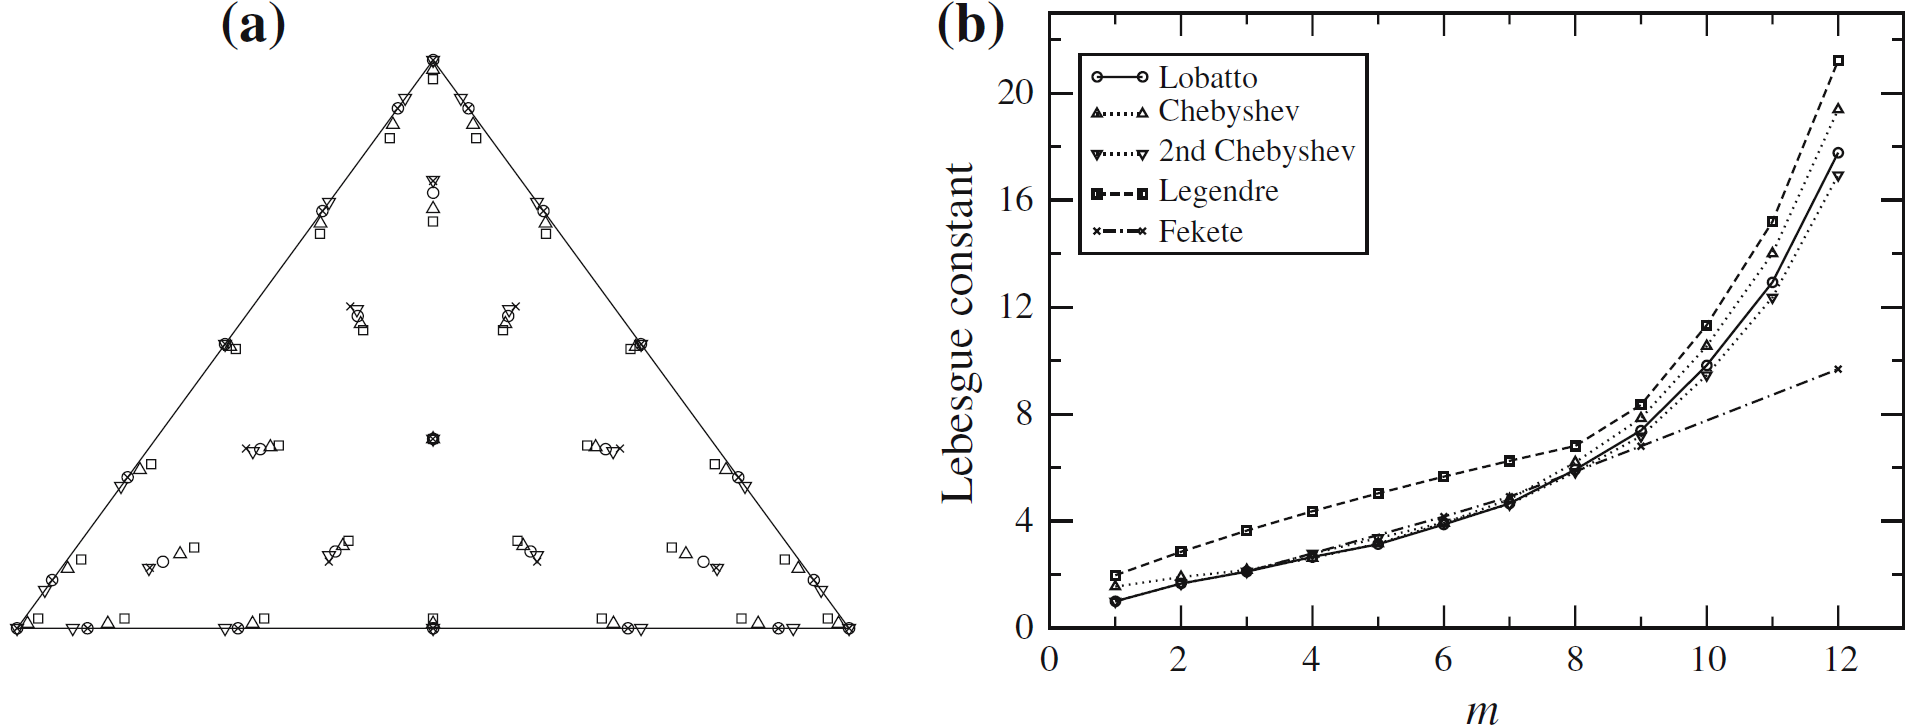
\includegraphics[width=0.9\linewidth]{includefiles/triangle nodes compare.png}
		\caption{
			三角形上 \(\mathscr{P}^{m}\) 多项式配点集合对比\cite{10.1007/s10665-006-9063-0}：
			(a) \(m = 6\) 时的 5 种不同配点集：Lobatto 点(圆)、Chebyshev 点(正三角)、第二类 Chebyshev 点(倒三角)、Legendre 点(方)、Fekete 点(叉)；
			(b) 当 \(1 \leqslant m \leqslant 12\) 时的插值 Lebesgue 常数
		}
	\end{center}
\end{figure}

如果在张量积参考单元上使用 \(\mathscr{Q}^k\) 多项式空间，并使用多线性映射映射到物理单元\cite{10.1090/s0025-5718-02-01439-4}，则可以直接使用 Gauss-Lobatto 点(使得迹算子稀疏化、支持 static condensation\cite{10.2514/3.2874})或者 Gauss-Legendre 点，这些积分点有很多成熟、高效的计算方式\cite{10.1137/140954969, 10.1137/S1064827500379690, 10.1017/S0962492920000045}，质量矩阵也有近似的对角取法\cite{10.1002/fld.2376}。其优点是可以利用张量积的结构加速计算，缺点是单元的 Jacobian 不是常数、总自由度较高。

% Aside from the use of tensor products of one-dimensional Gaussian formulas, there is no general procedure for obtaining multidimensional quadrature formulas. Optimal quadrature formulas, those that minimize the number of quadrature points and possess desirable properties such as symmetry and low condition number, are not readily available, and the development of such formulas is an active area of research.

由于其便于理解(所有的待解的变量都是点值)的特性，Nodal DG\cite{10.1007/978-0-387-72067-8}是 DG 的一种流行的具体实现方法。我们这里采用Nodal DG方法，并采用单纯形仿射单元。在二维，这样的方法属于三角谱配点法(TSEM, triangular spectral collocation method)或者三角伪谱法(triangular pseudo-spectral method)。


\subsubsection{2D Case Matrix}

取参考单元 \(\widehat{K}\) 是以 \(\B{P_1 = (1,0)^T, P_2 = (0,1)^T, P_3 = (0,0)^T}\) 为顶点的的标准单纯形：
\begin{equation}
	\widehat{K} = \B{\left(\lambda_1, \lambda_2\right) \big| 0\leqslant \lambda_1, \lambda_2 \leqslant \lambda_1 + \lambda_2 \leqslant 1}
\end{equation}
其三条边的单位外法向分别是 \(\widehat{\bm n}_1 = (-1, 0)^T\)，\(\widehat{\bm n}_2 = (0, -1)^T\)，\(\widehat{\bm n}_3 = (\frac{1}{\sqrt{2}}, \frac{1}{\sqrt{2}})^T\).

取物理单元 \(K\) 是以 \(\B{P_{j} = \left(x_{j}, y_{j}\right)^T \big| 1\leqslant j \leqslant 3}\) 为顶点的三角形，参考单元 \(\widehat{K}\) 的坐标 \(\bm\lambda = \left(\lambda_1, \lambda_2\right)\) 到物理单元 \(K\) 的坐标 \(\bm x = \left(x, y\right)\) 的仿射映射 \(\Phi: \widehat{K} \mapsto K\) 和其 Jacobi 矩阵(常矩阵)分别为：
\begin{equation}
	\begin{pmatrix}
		x(\xi, \eta) \\
		y(\xi, \eta)
	\end{pmatrix}
	= \begin{pmatrix}
		x_1 & x_2 & x_3 \\
		y_1 & y_2 & y_3
	\end{pmatrix}
	\begin{pmatrix}
		\lambda_1 \\
		\lambda_2 \\
		\lambda_3
	\end{pmatrix}
	= \begin{pmatrix}
		x_3 \\ y_3
	\end{pmatrix}
	+ \begin{pmatrix}
		x_1 - x_3 & x_2 - x_3 \\
		y_1 - y_3 & y_2 - y_3
	\end{pmatrix}
	\begin{pmatrix}
		\lambda_1 \\ \lambda_2
	\end{pmatrix}
\end{equation}
\begin{equation}
	\bm J[\Phi]
	= \begin{pmatrix}
		\frac{\partial x}{\partial \lambda_1} & \frac{\partial x}{\partial \lambda_2} \\
		\frac{\partial y}{\partial \lambda_1} & \frac{\partial y}{\partial \lambda_2}
	\end{pmatrix}
	= \begin{pmatrix}
		x_1 - x_3 & x_2 - x_3 \\
		y_1 - y_3 & y_2 - y_3
	\end{pmatrix}
\end{equation}
这里，重心坐标为 \(\B{\left(\lambda_1, \lambda_2, \lambda_3\right) \big| \lambda_j \geqslant 0, \lambda_1 + \lambda_2 + \lambda_3 = 1}\)，单纯形单元 \(K\) 的有向面积为 \(\frac{1}{2}\det \bm J[\Phi]\) (当有向面积为正时，才是合法的单元)，其三条边的单位外法向分别是
\begin{equation}
	\bm n_j = \frac{\left(\begin{smallmatrix} 0 & 1 \\ -1 & 0 \end{smallmatrix}\right)(P_{j+2} - P_{j+1})}{\abs{P_{j+2} - P_{j+1}}}
\end{equation}
这里下标以 3 为轮换周期。

我们下面考虑单元上的有限元空间 \(V(K)\). 记 \(V(\widehat{K})\) 是参考单元上相应的函数空间，定义拉回(pull-back)算子 \(\Phi^{\ast}\) 和前推(push-forward)算子 \(\Phi_{\ast}\) 如下：
\begin{subequations}
	\begin{eqnarray}
		&& \Phi^{\ast}: V(K) \mapsto V(\widehat{K}): u(\bm x) \mapsto \widehat{u}(\bm\lambda) = u(\Phi(\bm\lambda)) \\
		&& \Phi_{\ast}: V(\widehat{K}) \mapsto V(K): \widehat{u}(\bm\lambda) \mapsto u(\bm x) = \widehat{u}(\Phi^{-1}(\bm x))
	\end{eqnarray}
\end{subequations}
易见，\(\Phi^{\ast}\Phi_{\ast} = \Phi_{\ast}\Phi^{\ast} = I\)，且 \(k\) 次多项式空间具有仿射等价性：

\begin{proposition}
	对于仿射单元 \(K\)，设参考单元为 \(\widehat{K}\)，对应的仿射映射为 \(\Phi\)，那么：
	\begin{itemize}
		\item \(\mathscr{P}^{k}(K) = \Phi_{\ast} \mathscr{P}^{k}(\widehat{K})\)
		\item \(\mathscr{P}^{k}(\widehat{K}) = \Phi^{\ast} \mathscr{P}^{k}(K)\)
	\end{itemize}
\end{proposition}

取参考函数空间 \(\mathscr{P}^{k}(\widehat{K})\) 的基函数 \(\B{\widehat{\phi}_{j} \big| j=1,\cdots,N(k)}\)\footnote{由于我们使用 Nodal DG 方法，这里的基函数应选取配点基函数。}，这里 \(N_{k} = \dim\mathscr{P}^{k}(\widehat{K})\). 设 \(\widehat{\bm N}(\bm\lambda)\) 为基函数向量；\(\widehat{\bm M}\) 是其质量矩阵；\(\widehat{\bm D}_{1}\)，\(\widehat{\bm D}_{2}\) 是其微分关系矩阵，也即：
\begin{subequations}
	\begin{eqnarray}
		&& \widehat{\bm N}(\bm\lambda) = \begin{pmatrix}
			\phi_1(\bm\lambda) & \cdots & \phi_{N_{k}(\bm\lambda)}
		\end{pmatrix} \\
		&& \widehat{\bm M} = \int_{\widehat{K}} \widehat{\bm N}(\bm\lambda)^T \widehat{\bm N}(\bm\lambda) \d\lambda \\
		&& \frac{\partial}{\partial\lambda_1} \widehat{\bm N}(\bm\lambda) = \widehat{\bm N}(\bm\lambda) \widehat{\bm D}_1, \quad \frac{\partial}{\partial\lambda_2} \widehat{\bm N}(\bm\lambda) = \widehat{\bm N}(\bm\lambda) \widehat{\bm D}_2
	\end{eqnarray}
\end{subequations}

对应地，物理单元 \(K\) 上的基函数向量 \(\bm N_{K}(\bm x)\)、质量矩阵 \(\bm M_{K}\)、微分关系矩阵 \(\bm D_{K,1}, \bm D_{K,2}\) 的定义是：
\begin{subequations}
	\begin{eqnarray}
		&& \bm N_{K}(\bm x) = \widehat{\bm N}(\Phi^{-1}(\bm x)) = \Phi_{\ast} \bm N_{k}(\bm x) \\
		&& \bm M_{K} = \int_{K} \bm N_{K}(\bm x)^T \bm N_{K}(\bm x) \d\bm x \\
		&& \frac{\partial}{\partial x}\bm N_{K}(\bm x) = \bm N_{K}(\bm x)\bm D_{K,1}, \quad \frac{\partial}{\partial y}\bm N_{K}(\bm x) = \bm N_{K}(\bm x)\bm D_{K,2}
	\end{eqnarray}
\end{subequations}
满足：
\begin{subequations}
	\begin{eqnarray}
		&& \bm M_{K} = \det(\bm J[\Phi]) \widehat{\bm M} \\
		&& \begin{pmatrix}
			\bm D_{K, 1} & \bm D_{K, 2}
		\end{pmatrix}
		= \begin{pmatrix}
			\widehat{\bm D}_{1} & \widehat{\bm D}_{2}
		\end{pmatrix}
		\left(\bm J[\Phi^{-1}] \otimes \bm I_{(N_{k})}\right)
	\end{eqnarray}
\end{subequations}
这里，Jacobi 矩阵求逆公式为 \(\bm J[\Phi^{-1}] = \bm J[\Phi]^{-1}(\Phi)\).



\subsection{The Local DG Method}


\subsubsection{The LDG Formulation}

在求解对称的椭圆问题时，在收敛阶相同时，CG 方法和对称的 DG 方法的矩阵条件数渐进同阶，而不对称的 DG 方法例如 NIPG 需要更大的惩罚参数，导致条件数很高。对称的 DG 方法中，LDG 方法和 IPDG 方法都易于实现，且稳定、相容、守恒、最优收敛。LDG 方法的矩阵存储量是 IPDG 的至多 2.5 倍(在 2D 三角网格下)\cite{10.1137/S1064827501388339}，但是 LDG 的优势在于惩罚参数的选取可以与网格无关，且辅助变量 \(\sigma_{h}\) 可以局部地用原始变量 \(u_{h}\) 表示出来(在定态求解时，可以使用 Schur 补技巧以减小计算量；在显式时间推进时，可以只需要多次求解局部小型方程组)。另外，DG 方法的特性使得其容易获得局部守恒性质，这在计算流体力学中对于长时间模拟的稳定性和准确性有重要作用，而 CG 方法需要复杂的处理\cite{10.1137/060666305}才能局部守恒。

LDG 格式的数值通量\cite{10.1137/S0036142997316712}为：
\begin{subequations}\label{LDG numerical flux}
	\begin{eqnarray}
		&& \widehat{\sigma}_{h}\big|_{e} = \begin{cases}
			\avg{\sigma_{h}} - \bm C_{12} \jump{\sigma_{h}} - C_{11} \jump{u_{h}}, & e \in \mathcal{E}_{h}^{o} \\
			\sigma_{h} - C_{11} \left(u_{h} - g_{D}\right)\bm{n}, & e \in \mathcal{E}_{h}^{D} \\
			\bm g_{N}, & e \in \mathcal{E}_{h}^{N}
		\end{cases} \\
		&& \widehat{u}_{h}\big|_{e} = \begin{cases}
			\avg{u_{h}} + \bm C_{12} \cdot \jump{u_{h}} - C_{22} \jump{\sigma_{h}}, & e \in \mathcal{E}_{h}^{o} \\
			g_{D}, & e \in \mathcal{E}_{h}^{D} \\
			u_{h} - C_{22} \left(\sigma_{h} - g_{N}\right) \cdot \bm n, & e \in \mathcal{E}_{h}^{N}
		\end{cases}
	\end{eqnarray}
\end{subequations}
这里，\(C_{11}, \bm C_{12}, C_{22}\) 在每条边 \(e \in \mathcal{E}_{h}\) 上是常值\footnote{在边界面 \(e\in\mathcal{E}_{h}^{\partial}\) 上，\(\bm C_{12}\) 未定义。}。特别地，当且仅当 \(C_{22} \equiv 0\) 时，可以局部地通过 \(u_{h}\) 求出 \(\sigma_{h}\)，整套方法才是 LDG 方法。

LDG 有误差估计\cite{10.1137/S0036142900371003}：对于一般的任意网格情形而言，当 \(\bm C_{12} = \mathcal{O}(1)\)时，\(\bm C_{12}\) 对代数方程组的可解性和误差估计无影响；当 \(C_{11} > 0\) 时，代数方程组可解；当 \(C_{11} = \mathcal{\Theta}(h^{-1})\) 时，对光滑解 \(\left(\sigma, u\right)\) 的 \(L^2\) 误差阶为 \(\left(k, k+1\right)\)；当 \(C_{11} = \mathcal{\Theta}(1)\) 时，对光滑解 \(\left(\sigma, u\right)\) 的 \(L^2\) 误差阶为 \(\left(k, k+\frac{1}{2}\right)\)；当 \(k\geqslant 1\) 时数值解收敛。同时，恰当地选取 \(\bm C_{12}\) 可以减小模板，从而减少矩阵非零元个数，例如取 \(\bm C_{12}\) 使得 \(\bm C_{12}\cdot\bm n \equiv \pm\frac{1}{2}\) \cite{10.1137/070685518}.

为了减小数值耗散，当使用单纯形单元时，实际上只需要 \(C_{11}\big|_{\Gamma^{D}} = \mathcal{\Theta}(h^{-1})\) 且 \(C_{11}\big|_{\Gamma} \geqslant 0\)，同时每一个单元的至少一条边 \(e\) 满足 \(\bm C_{12}\cdot\bm n = \frac{1}{2}\) 或者 \(e\in\mathcal{E}_{h} \backslash \mathcal{E}_{h}^{o}\)，即可达到对光滑 \(\left(\sigma, u\right)\) 的 \(\left(k, k+1\right)\) 阶收敛(\(k>0\))，此格式被称作 MD-LDG 格式\cite{10.1007/s10915-007-9130-3}。

取空间为：
\begin{subequations}
	\begin{eqnarray}
		&& \Sigma_{h} = \bigoplus_{K\in\mathcal{E}_{h}} \Sigma(K) = \bigoplus_{K\in\mathcal{E}_{h}} \left(\mathscr{P}^{k}(K)\right)^d \\
		&& V_{h} = \bigoplus_{K\in\mathcal{E}_{h}} V(K) = \bigoplus_{K\in\mathcal{E}_{h}} \mathscr{P}^{k}(K)
	\end{eqnarray}
\end{subequations}
将数值通量\eqref{LDG numerical flux}代入 DG 格式\eqref{Global DG Scheme}，LDG 格式可以写作\cite{10.1137/S0036142900371003}：

\begin{subequations}\label{LDG weak form}
	\begin{equation}
		\begin{aligned}
			& \text{find \(\left(\sigma_{h}, u_{h}\right)  \in \Sigma_{h} \times V_{h}\) such that \(\forall \left(\tau_{h}, v_{h}\right) \in \Sigma_{h} \times V_{h}\):} \\
			& \begin{cases}
				a_{h}\left(\sigma_{h}, \tau_h\right) + b_{h}\left(\tau_{h}, u_{h}\right) = F_{h}\left(\tau_{h}\right) \\
				b_{h}\left(\sigma_{h}, v_{h}\right) - c_{h}\left(u_{h}, v_{h}\right) = - G_{h}\left(v_{h}\right)
			\end{cases}
		\end{aligned}
	\end{equation}
	其中：
	\begin{eqnarray}
		&& a_{h}\left(\sigma_{h}, \tau_{h}\right) = \sum_{K\in\mathcal{T}_{h}} \int_{K} \sigma_{h} \cdot \tau_{h} \d x + \int_{\Gamma^{o}} C_{22} \jump{\sigma_{h}} \jump{\tau_{h}} \d s + \int_{\Gamma^{N}} C_{22} (\sigma_{h} \cdot \bm n) (\tau_{h} \cdot \bm n) \d s \\
		&& \begin{aligned}
			b_{h}\left(\tau_{h}, u_{h}\right)
			& = \sum_{K\in\mathcal{T}_{h}} \int_{K} u_{h} \nabla \cdot \tau_{h} \d x - \int_{\Gamma^{o}} \left(\avg{u_{h}} + \bm{C}_{12} \cdot \jump{u_{h}}\right) \jump{\tau_{h}} \d s - \int_{\Gamma^{N}} u_{h} \tau_{h} \cdot n \d s \\
			& = -\sum_{K\in\mathcal{T}_{h}} \int_{K} \tau_{h} \cdot \nabla u_{h} \d x + \int_{\Gamma^{o}} \left(\avg{\tau_{h}} - \bm C_{12} \jump{\tau_{h}}\right) \cdot \jump{u_{h}} \d s + \int_{\Gamma^{D}} u_{h} \tau_{h} \cdot \bm n \d s
		\end{aligned} \\
		&& c_{h}\left(u_{h}, v_{h}\right) = \int_{\Gamma^{o}} C_{11} \jump{u_{h}} \cdot \jump{v_{h}} \d s + \int_{\Gamma^{D}} C_{11} u_{h} v_{h} \d s \\
		&& F_{h}(\tau_{h}) = \int_{\Gamma^{D}} g_{D} \tau_{h} \cdot \bm n \d s + \int_{\Gamma^{N}} C_{22} \left(\bm g_{N} \cdot \bm n\right) \left(\tau_{h} \cdot \bm n\right) \d s \\
		&& G_{h}(v_{h}) = \sum_{K\in\mathcal{T}_{h}} \int_{K} f v_{h} \d x + \int_{\Gamma^{D}} C_{11} g_{D} v_{h} \d s + \int_{\Gamma^{N}} v_{h} \bm g_{N} \cdot \bm n \d s
	\end{eqnarray}
\end{subequations}

\begin{remark}
	LDG 格式中，Dirichlet 边界条件并不是强制施加的，而是采用了一个惩罚项来施加，惩罚系数为 \(C_{11}\). 这种惩罚方法与 Nitsche 方法类似\cite{10.1007/BF02995904}。
\end{remark}

LDG 方程组\eqref{LDG weak form}等价的(带稳定项的)鞍点问题为\footnote{该鞍点问题属于 purturbed saddle-point problem，不能等价于关于 \(\tau_{h}\) 的限制优化问题。}：
\begin{subequations}\label{LDG saddle-point problem}
	\begin{equation}
		\begin{aligned}
			& \text{find \(\left(\sigma_{h}, u_{h}\right) \in \Sigma_{h} \times V_{h}\) such that \(\forall \left(\tau_{h}, v_{h}\right) \in \Sigma_{h} \times V_{h}\):} \\
			& L_{h}\left(\sigma_{h}, v_{h}\right) \leqslant L_{h}\left(\sigma_{h}, u_{h}\right) \leqslant L_{h}\left(\tau_{h}, u_{h}\right)
		\end{aligned}
	\end{equation}
	其中：
	\begin{equation}
		L_{h}\left(\tau_{h}, v_{h}\right)
		= \frac{1}{2}a_{h}\left(\tau_{h}, \tau_{h}\right) + b_{h}\left(\tau_{h}, v_{h}\right) - \frac{1}{2}c_{h}\left(v_{h}, v_{h}\right) - F_{h}\left(\tau_{h}\right) + G_{h}\left(v_{h}\right)
	\end{equation}
\end{subequations}


\begin{theorem}[Well-posedness\cite{10.1137/S0036142900371003, 10.1007/s10915-007-9130-3}]
	当 \(C_{11}, C_{22} \geqslant 0\) 时，若至少有一条边上是 Dirichlet 边界条件，且以下两条至少成立一条：
	\begin{itemize}
		\item \(C_{11} > 0\) 恒成立。
		\item 单元都是单纯形，\(C_{11} > 0\) 在 Dirichlet 边界上成立，同时每个单元有至少一条边 \(e\) 满足两条件之一：(1) \(\bm C_{12}\cdot\bm n = \frac{1}{2}\)，(2) \(e\in\mathcal{E}_{h}\backslash\mathcal{E}_{h}^{o}\).
	\end{itemize}
	那么 LDG 问题\eqref{LDG weak form}存在唯一解。

	\begin{proof}
		对于此线性问题，我们只需要证明当右端项全部为 \(0\) 时，方程仅有平凡解。事实上，当右端项全部为 \(0\) 时，取测试函数 \(\left(\tau_{h}, v_{h}\right) = \left(\sigma_{h}, u_{h}\right)\)，我们有：
		\begin{equation*}
			\norm{\sigma_{h}}_{L^2(\Omega)}^2 + \norm{\jump{\sigma_{h}}}_{L^2(\Gamma^{o}, C_{22})}^2 + \norm{\sigma_{h}\cdot\bm n}_{L^2(\Gamma^{N}, C_{22})}^2 + \norm{\jump{u_{h}}}_{L^2(\Gamma^{o}, C_{11})}^2 + \norm{u_{h}}_{L^2(\Gamma^{D}, C_{11})}^2 = 0
		\end{equation*}
		这说明 \(\sigma_{h} = 0\)，\(b_{h}(u_{h}, \cdot) = 0\)，\(\forall e \in \mathcal{E}_{h}^{o}, C_{11}\jump{u_{h}} = \bm 0\)，\(\forall e \in \mathcal{E}_{h}^{D}, C_{11}u_{h} = 0\). 

		若 \(C_{11} > 0\) 恒成立，那么易推出 \(u_{h} \equiv 0\)，得证。

		若仅要求 \(C_{11}\big|_{\Gamma^{D}} > 0\)，那么 \(u_{h}\big|_{\Gamma^{D}} = 0\). 注意到 \(b_{h}(u_{h}, \cdot) = 0\) 等价于：
		\begin{equation*}
			\begin{aligned}
				& \forall K, \forall \tau_{h} \in \Sigma(K): \\
				& \int_{K} \tau_{h} \cdot \nabla u_{h} \d x + \oint_{\partial K} \left(\widehat{u}_{h} - u_{h}\right) \tau_{h} \cdot \bm n \d s = 0
			\end{aligned}
		\end{equation*}
		同时，此时有：
		\begin{equation*}
			\widehat{u}_{h} - u_{h}
			=\begin{cases}
				\left(\bm C_{12} - \frac{\bm n_{e}}{2}\right)\cdot\jump{u_{h}} - C_{22}\jump{\sigma_{h}} = \left(\bm C_{12} - \frac{\bm n_{e}}{2}\right)\cdot\jump{u_{h}}, & e\in\mathcal{E}_{h}^{o} \\
				g_{D} - u_{h} = -u_{h} = 0, & e\in\mathcal{E}_{h}^{D} \\
				0, & e\in\mathcal{E}_{h}^{N}
			\end{cases}
		\end{equation*}
		因此，当单元 \(K\) 都是单纯形时，使用测试函数 \(\tau_{h} \in \Sigma_{h}\) 满足\cite{10.1007/s10915-007-9130-3}：
		\begin{equation*}
			\forall K \in \mathcal{T}_{h},
			\begin{cases}
				\left(\tau_{h} - \nabla u_{h}\right) \perp \left(\mathscr{P}^{k-1}(K)\right)^d \\
				\left(\tau_{h} \cdot \bm n_{e} - \left(\widehat{u}_{h} - u_{h}\right)\right) \perp \mathscr{P}^{k}(e), & \forall e \in \B{e_1, \cdots, e_d} \subsetneqq \mathcal{E}_{h}^{K}
			\end{cases}
		\end{equation*}
		此处，取 \(K\) 的边 \(e_{d+1}\) 使得其上有 \(\widehat{u}_{h} - u_{h} = 0\). 那么：
		\begin{equation*}
			0 = b_{h}\left(u_{h}, \tau_{h}\right)
			= - \sum_{K \in \mathcal{T}_{h}} \left(\norm{\nabla u_{h}}_{L^2(K)}^2 + \norm{\widehat{u}_{h} - u_{h}}_{L^2(\partial K)}^2\right)
		\end{equation*}
		因此，\(u_{h} = C_{K}\) 且 \(\widehat{u}_{h} - u_{h} = 0\)，同时可知 \(\jump{u_{h}}\big|_{\Gamma^{o}} = \bm 0\)，从而 \(u_{h} \equiv C\). 因为在 Dirichlet 边界处有 \(u_{h}\big|_{\Gamma^{D}} = 0\)，于是 \(u_{h} \equiv 0\)，得证。
	\end{proof}
\end{theorem}


\subsubsection{Numerical Discretization}

LDG 方程组\eqref{LDG weak form}对应的线性代数方程组为：
\begin{equation}\label{LDG linear equations}
	\begin{pmatrix}
		\bm A & \bm B^T \\
		\bm B & -\bm C
	\end{pmatrix}
	\begin{pmatrix}
		\bm\sigma \\
		\bm u
	\end{pmatrix}
	= \begin{pmatrix}
		\bm F \\
		-\bm G
	 \end{pmatrix}
\end{equation}
这里，\(\bm A\) 是 \(\Sigma_{h}\) 的质量矩阵，对称正定、分块对角，可以显式求逆。利用 Schur 补，可以将 \(\bm\sigma\) 用 \(\bm u\) 局部地显示表示(模板只涉及自己与邻居单元)，这是 LDG 的特性：

\begin{lemma}[Schur complement]
	LDG 线性代数方程组\eqref{LDG linear equations}的系数矩阵是对称不定的，其 Schur 补公式和求逆公式如下给出，并且 Schur 补矩阵 \(\bm S = \bm C + \bm B \bm A^{-1} \bm B^{T}\) 是对称正定的。
	\begin{equation}\label{LDG Schur complement}
		\begin{pmatrix}
			\bm A & \bm B^T \\
			\bm B & -\bm C
		\end{pmatrix}
		= \begin{pmatrix}
			\bm I & \bm 0 \\
			\bm B \bm A^{-1} & \bm I
		\end{pmatrix}
		\begin{pmatrix}
			\bm A & \bm 0 \\
			\bm 0 & -\bm S
		\end{pmatrix}
		\begin{pmatrix}
			\bm I & \bm A^{-1} \bm B^{T} \\
			\bm 0 & \bm I
		\end{pmatrix}
	\end{equation}
	\begin{equation}\label{LDG inverse matrix}
		\begin{pmatrix}
			\bm A & \bm B^T \\
			\bm B & -\bm C
		\end{pmatrix}^{-1}
		= \begin{pmatrix}
			\bm I & -\bm A^{-1} \bm B^{T} \\
			\bm 0 & \bm I
		\end{pmatrix}
		\begin{pmatrix}
			\bm A^{-1} & \bm 0 \\
			\bm 0 & -\bm S^{-1}
		\end{pmatrix}
		\begin{pmatrix}
			\bm I & \bm 0 \\
			-\bm B \bm A^{-1} & \bm I
		\end{pmatrix}
	\end{equation}
\end{lemma}


\subsubsection{Numerical Example (1D Dirichlet)}

区域 \(\Omega = [0,3\pi]\)，准确解 \(u(x) = \exp\left(\sin(x)\right)\)，采用 Dirichlet 边界条件。空间剖分使用均匀网格，用 \(N\) 表示单元个数，\(k\) 表示多项式次数。取罚参数 \(C_{11} = \eta h^{-\alpha}\)，其中 \(\eta = 1\). 我们使用 Legendre 配点法，使用 Gauss-Legendre 公式进行源项 \(f\) 的数值积分和误差测量。测试结果如表所示：

\begin{table}[H]
	\begin{center}
		\resizebox{\linewidth}{!}{
		\begin{tabular}{c | c c | c c | c c | c c }
			\toprule

			\multirow{2}{*}{\(N\)} & \multicolumn{4}{c |}{\(C_{12} = 0\)} & \multicolumn{4}{c}{\(C_{12} = \frac{1}{2}\)} \\
			& \(\norm{u - u_{h}}_{L^2}\) & order & \(\norm{\sigma -\sigma_{h}}_{L^2}\) & order & \(\norm{u - u_{h}}_{L^2}\) & order & \(\norm{\sigma -\sigma_{h}}_{L^2}\) & order \\

			\midrule

			16 & 8.8771e-01 & - & 1.0487e+00 & - & 1.0931e+00 & - & 1.4214e+00 & - \\
			32 & 5.9567e-01 & 0.5756 & 6.5089e-01 & 0.6881 & 6.9041e-01 & 0.6629 & 8.4408e-01 & 0.7519 \\
			64 & 3.5480e-01 & 0.7475 & 3.7580e-01 & 0.7925 & 3.9250e-01 & 0.8148 & 4.6841e-01 & 0.8496 \\
			128 & 1.9538e-01 & 0.8607 & 2.0412e-01 & 0.8805 & 2.1032e-01 & 0.9001 & 2.4822e-01 & 0.9161 \\
			256 & 1.0280e-01 & 0.9265 & 1.0671e-01 & 0.9357 & 1.0904e-01 & 0.9477 & 1.2799e-01 & 0.9556 \\
			512 & 5.2766e-02 & 0.9622 & 5.4605e-02 & 0.9666 & 5.5541e-02 & 0.9732 & 6.5021e-02 & 0.9771 \\

			\bottomrule
		\end{tabular}
		}
		\caption{\(k = 0\)，\(\alpha = 0\)}
	\end{center}
\end{table}

\begin{table}[H]
	\begin{center}
		\resizebox{\linewidth}{!}{
		\begin{tabular}{c | c c | c c | c c | c c }
			\toprule

			\multirow{2}{*}{\(N\)} & \multicolumn{4}{c |}{\(C_{12} = 0\)} & \multicolumn{4}{c}{\(C_{12} = \frac{1}{2}\)} \\
			& \(\norm{u - u_{h}}_{L^2}\) & order & \(\norm{\sigma -\sigma_{h}}_{L^2}\) & order & \(\norm{u - u_{h}}_{L^2}\) & order & \(\norm{\sigma -\sigma_{h}}_{L^2}\) & order \\

			\midrule

			16 & 1.0075e-01 & - & 5.2555e-01 & - & 6.3392e-02 & - & 2.0899e-01 & - \\
			32 & 2.7394e-02 & 1.7940 & 2.9980e-01 & 0.7733 & 1.4799e-02 & 2.0040 & 8.9115e-02 & 1.1741 \\
			64 & 7.0357e-03 & 1.9169 & 1.6003e-01 & 0.8852 & 3.6018e-03 & 1.9927 & 4.2322e-02 & 1.0500 \\
			128 & 1.7647e-03 & 1.9727 & 8.1839e-02 & 0.9566 & 8.8855e-04 & 1.9964 & 2.0821e-02 & 1.0118 \\
			256 & 4.4035e-04 & 1.9914 & 4.1170e-02 & 0.9856 & 2.2066e-04 & 1.9983 & 1.0353e-02 & 1.0024 \\
			512 & 1.0988e-04 & 1.9971 & 2.0616e-02 & 0.9950 & 5.4982e-05 & 1.9992 & 5.1652e-03 & 1.0003 \\

			\bottomrule
		\end{tabular}
		}
		\caption{\(k = 1\)，\(\alpha = -1\)}
	\end{center}
\end{table}

\begin{table}[H]
	\begin{center}
		\resizebox{\linewidth}{!}{
		\begin{tabular}{c | c c | c c | c c | c c }
			\toprule

			\multirow{2}{*}{\(N\)} & \multicolumn{4}{c |}{\(C_{12} = 0\)} & \multicolumn{4}{c}{\(C_{12} = \frac{1}{2}\)} \\
			& \(\norm{u - u_{h}}_{L^2}\) & order & \(\norm{\sigma -\sigma_{h}}_{L^2}\) & order & \(\norm{u - u_{h}}_{L^2}\) & order & \(\norm{\sigma -\sigma_{h}}_{L^2}\) & order \\

			\midrule

			16 & 3.6665e-03 & - & 1.8931e-02 & - & 5.6514e-03 & - & 2.1373e-02 & - \\
			32 & 2.1157e-04 & 3.9293 & 3.9588e-03 & 2.1556 & 6.1604e-04 & 3.0531 & 4.2119e-03 & 2.2374 \\
			64 & 2.0045e-05 & 3.3231 & 9.5234e-04 & 2.0092 & 7.3413e-05 & 2.9997 & 9.6842e-04 & 2.0729 \\
			128 & 2.2933e-06 & 3.0925 & 2.3415e-04 & 2.0012 & 8.9682e-06 & 2.9989 & 2.3514e-04 & 2.0191 \\
			256 & 2.7861e-07 & 3.0239 & 5.8069e-05 & 2.0002 & 1.1081e-06 & 2.9997 & 5.8130e-05 & 2.0048 \\
			512 & 3.4478e-08 & 3.0060 & 1.4460e-05 & 2.0001 & 1.3772e-07 & 2.9999 & 1.4464e-05 & 2.0012 \\

			\bottomrule
		\end{tabular}
		}
		\caption{\(k = 2\)，\(\alpha = -1\)}
	\end{center}
\end{table}

\begin{table}[H]
	\begin{center}
		\resizebox{\linewidth}{!}{
		\begin{tabular}{c | c c | c c | c c | c c }
			\toprule

			\multirow{2}{*}{\(N\)} & \multicolumn{4}{c |}{\(C_{12} = 0\)} & \multicolumn{4}{c}{\(C_{12} = \frac{1}{2}\)} \\
			& \(\norm{u - u_{h}}_{L^2}\) & order & \(\norm{\sigma -\sigma_{h}}_{L^2}\) & order & \(\norm{u - u_{h}}_{L^2}\) & order & \(\norm{\sigma -\sigma_{h}}_{L^2}\) & order \\

			\midrule

			16 & 4.5438e-04 & - & 4.0165e-03 & - & 4.3583e-04 & - & 1.9235e-03 & - \\
			32 & 3.6328e-05 & 3.4801 & 7.5135e-04 & 2.3092 & 2.4772e-05 & 3.9501 & 1.7786e-04 & 3.2797 \\
			64 & 2.2516e-06 & 3.9215 & 1.2629e-04 & 2.5147 & 1.4661e-06 & 3.9866 & 1.9856e-05 & 3.0918 \\
			128 & 1.2699e-07 & 4.1014 & 1.7835e-05 & 2.7920 & 8.9077e-08 & 3.9952 & 2.3837e-06 & 3.0238 \\
			256 & 7.4788e-09 & 4.0628 & 2.3035e-06 & 2.9362 & 5.4873e-09 & 3.9982 & 2.9332e-07 & 3.0056 \\
			512 & 4.5714e-10 & 4.0207 & 2.8981e-07 & 2.9822 & 3.4057e-10 & 3.9988 & 3.6420e-08 & 3.0012 \\

			\bottomrule
		\end{tabular}
		}
		\caption{\(k = 3\)，\(\alpha = -1\)}
	\end{center}
\end{table}

\begin{table}[H]
	\begin{center}
		\resizebox{\linewidth}{!}{
		\begin{tabular}{c | c c | c c | c c | c c }
			\toprule

			\multirow{2}{*}{\(N\)} & \multicolumn{4}{c |}{\(C_{12} = 0\)} & \multicolumn{4}{c}{\(C_{12} = \frac{1}{2}\)} \\
			& \(\norm{u - u_{h}}_{L^2}\) & order & \(\norm{\sigma -\sigma_{h}}_{L^2}\) & order & \(\norm{u - u_{h}}_{L^2}\) & order & \(\norm{\sigma -\sigma_{h}}_{L^2}\) & order \\

			\midrule

			16 & 2.6600e-05 & - & 1.4240e-04 & - & 2.6326e-05 & - & 1.2055e-04 & - \\
			32 & 3.3233e-07 & 6.3227 & 5.6451e-06 & 4.6567 & 8.1399e-07 & 5.0153 & 6.1423e-06 & 4.2947 \\
			64 & 5.6330e-09 & 5.8826 & 3.4759e-07 & 4.0215 & 2.5655e-08 & 4.9877 & 3.5680e-07 & 4.1056 \\
			128 & 1.2346e-10 & 5.5117 & 2.1711e-08 & 4.0009 & 8.0434e-10 & 4.9953 & 2.1858e-08 & 4.0289 \\
			256 & 3.5767e-12 & 5.1093 & 1.3572e-09 & 3.9997 & 2.5194e-11 & 4.9966 & 1.3595e-09 & 4.0070 \\
			512 & 9.0223e-13 & 1.9871 & 8.4848e-11 & 3.9996 & 4.0796e-12 & 2.6266 & 8.4892e-11 & 4.0013 \\

			\bottomrule
		\end{tabular}
		}
		\caption{\(k = 4\)，\(\alpha = -1\)}
	\end{center}
\end{table}

数值结果基本符合文章\cite{10.1137/S0036142900371003}中的估计，不同的地方有：
\begin{itemize}
	\item 当 \(k\geqslant 0\)，\(\alpha = 0\)，\(C_{12} = \frac{1}{2}\) 时，观察到对 \(\left(\sigma, u\right)\) 的 \((k+1, k+1)\) 阶收敛，这符合笛卡尔网格上的超收敛结果\cite{10.1090/S0025-5718-01-01317-5, 10.1137/S0036142900371544}。
	\item 当 \(k \geqslant 0\)，\(\alpha = 0\) 时：\begin{itemize}
		\item 当 \(C_{12} = 0\) 时：若 \(k\) 是偶数，则观察到对 \(\left(\sigma, u\right)\) 的 \(\left(k+1, k+1\right)\) 阶收敛；若 \(k\) 是奇数，则观察到对 \(\left(\sigma, u\right)\) 的 \(\left(k, k+1\right)\) 阶收敛。
		\item 当 \(C_{12} \neq 0\) 时，观察到对 \(\left(\sigma, u\right)\) 的 \(\left(k+1, k+1\right)\) 阶收敛。
	\end{itemize}
	\item 当 \(k = 0\) 且 \(\alpha = -1\) 时，总不收敛。
\end{itemize}

我们又使用了不同的配点，测试矩阵的稀疏模式，分别输出了原始矩阵以及使用 local solver 之后的矩阵，如图\ref{1D LDG Legendre node spy}、\ref{1D LDG Lobatto node spy}所示，我们发现：
\begin{itemize}
	\item 当 \(C_{12} = \pm\frac{1}{2}\) 时，可以减少 \(\bm B\) 的非零元个数。
	\item 由于 \(\bm B\) 和 \(\bm C\) 中存在很多只依赖于单元的迹的算子，当配点使用了两端边界点时(例如 Lobatto 配点和等距配点)，\(\bm B\) 和 \(\bm C\) 可以变得更加稀疏。
\end{itemize}

\begin{figure}[H]
	\begin{center}
		\begin{subfigure}{0.49\linewidth}
			\begin{center}
				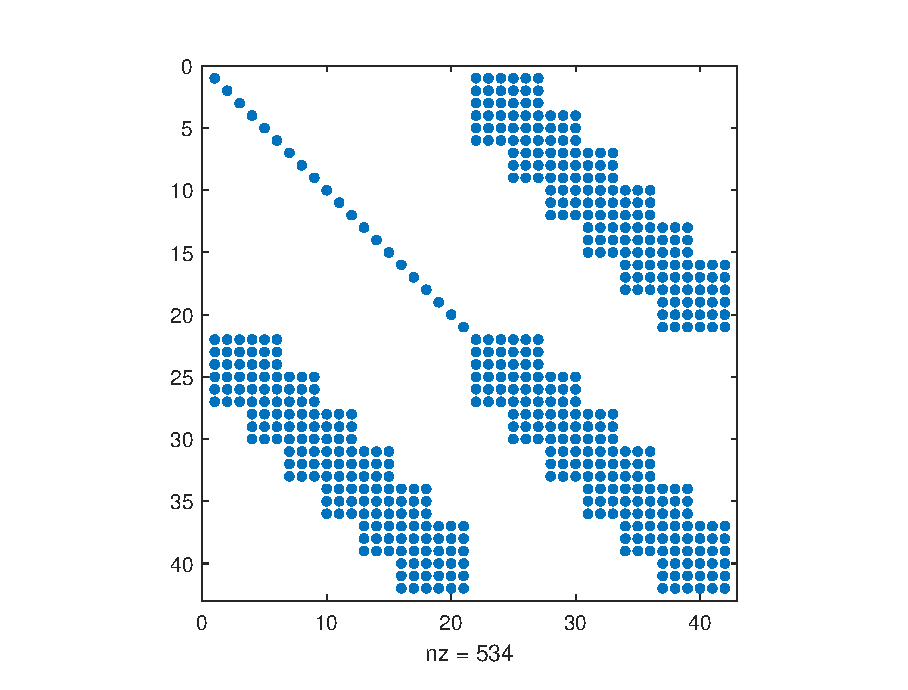
\includegraphics[width=\linewidth]{includefiles/1D poisson LDG spy/legendre c=00 direct.eps}
				\caption{\(C_{12} \neq \pm\frac{1}{2}\), original matrix}
			\end{center}
		\end{subfigure}
		\begin{subfigure}{0.49\linewidth}
			\begin{center}
				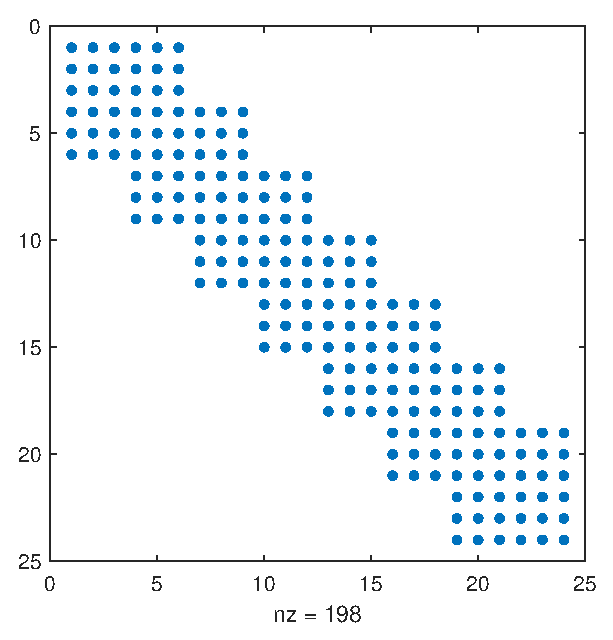
\includegraphics[width=\linewidth]{includefiles/1D poisson LDG spy/legendre c=05 reduce.eps}
				\caption{\(C_{12} \neq \pm\frac{1}{2}\), condensed matrix}
			\end{center}
		\end{subfigure}

		\begin{subfigure}{0.49\linewidth}
			\begin{center}
				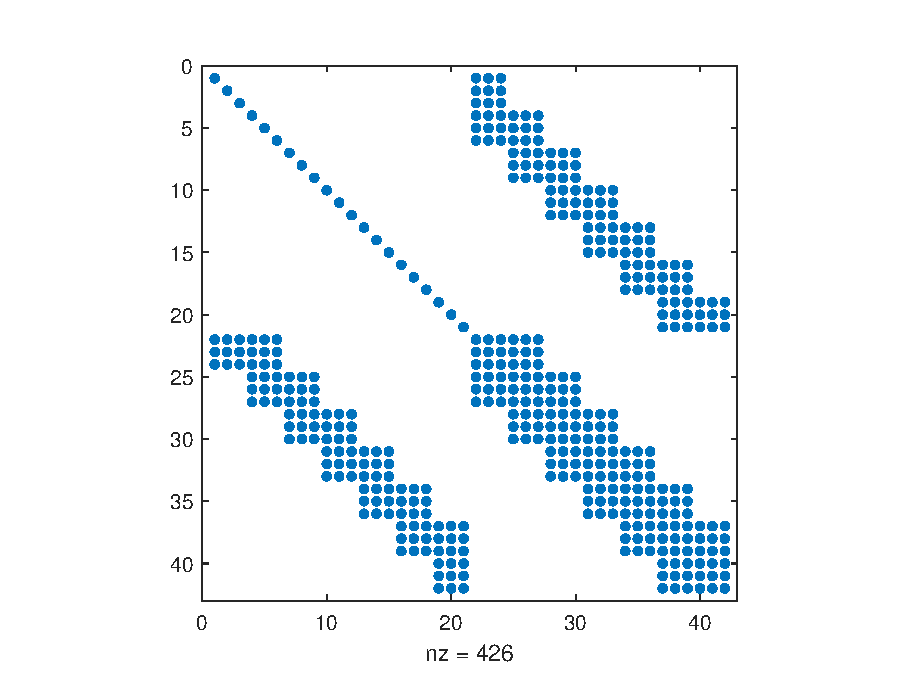
\includegraphics[width=\linewidth]{includefiles/1D poisson LDG spy/legendre c=05 direct.eps}
				\caption{\(C_{12} = \frac{1}{2}\), original matrix}
			\end{center}
		\end{subfigure}
		\begin{subfigure}{0.49\linewidth}
			\begin{center}
				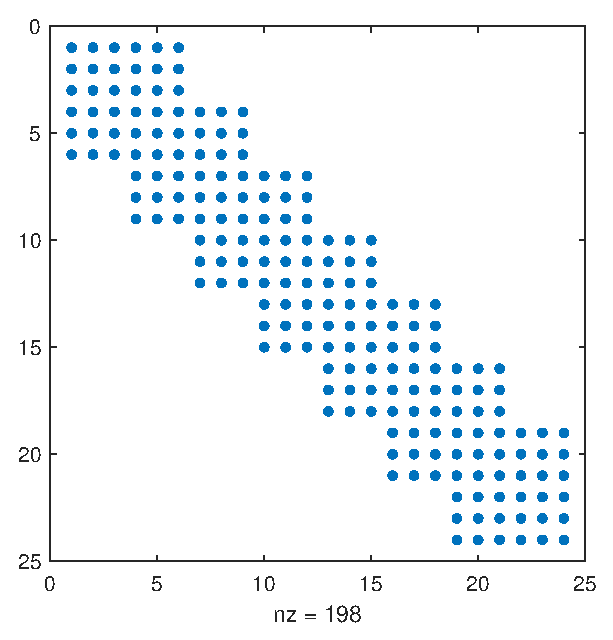
\includegraphics[width=\linewidth]{includefiles/1D poisson LDG spy/legendre c=05 reduce.eps}
				\caption{\(C_{12} = \frac{1}{2}\), condensed matrix}
			\end{center}
		\end{subfigure}
		\caption{Legendre nodes, \(k = 2\)，\(N = 8\)}
		\label{1D LDG Legendre node spy}
	\end{center}
\end{figure}

\begin{figure}[H]
	\begin{center}
		\begin{subfigure}{0.49\linewidth}
			\begin{center}
				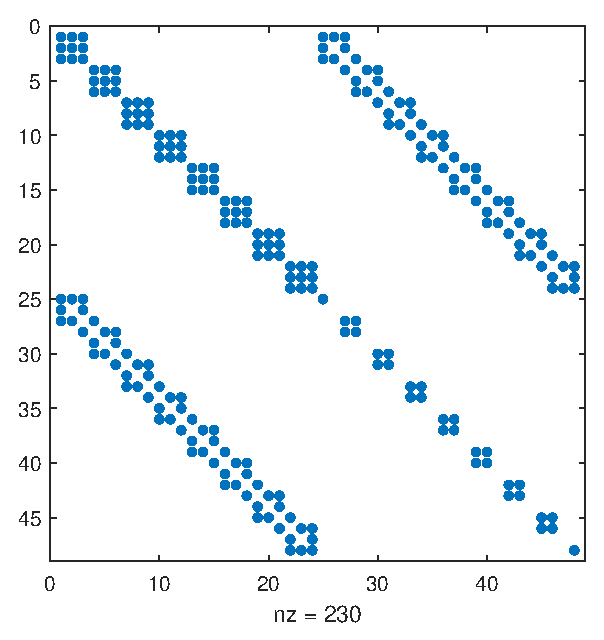
\includegraphics[width=\linewidth]{includefiles/1D poisson LDG spy/lobatto c=00 direct.eps}
				\caption{\(C_{12} \neq \pm\frac{1}{2}\), original matrix}
			\end{center}
		\end{subfigure}
		\begin{subfigure}{0.49\linewidth}
			\begin{center}
				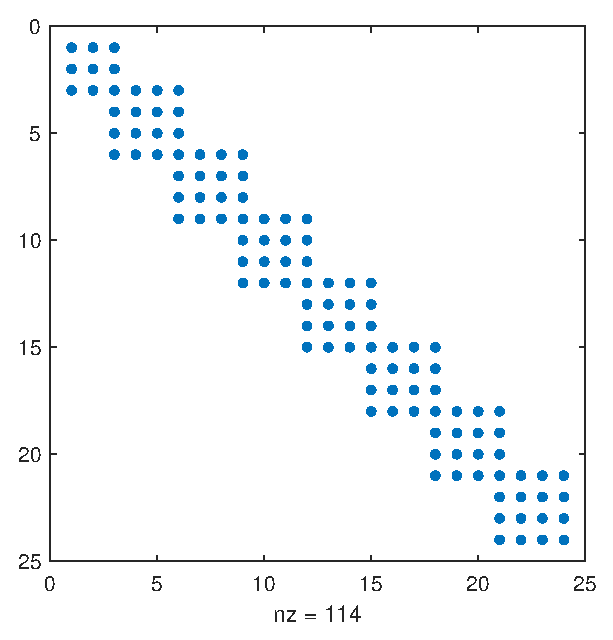
\includegraphics[width=\linewidth]{includefiles/1D poisson LDG spy/lobatto c=05 reduce.eps}
				\caption{\(C_{12} \neq \pm\frac{1}{2}\), condensed matrix}
			\end{center}
		\end{subfigure}

		\begin{subfigure}{0.49\linewidth}
			\begin{center}
				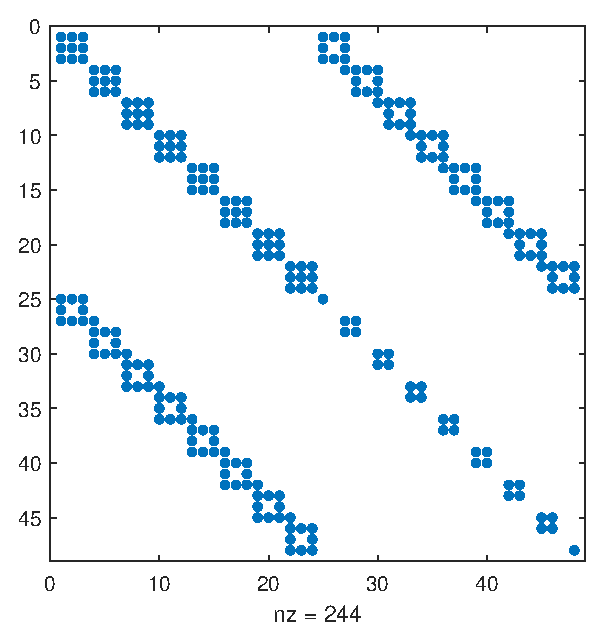
\includegraphics[width=\linewidth]{includefiles/1D poisson LDG spy/lobatto c=05 direct.eps}
				\caption{\(C_{12} = \frac{1}{2}\), original matrix}
			\end{center}
		\end{subfigure}
		\begin{subfigure}{0.49\linewidth}
			\begin{center}
				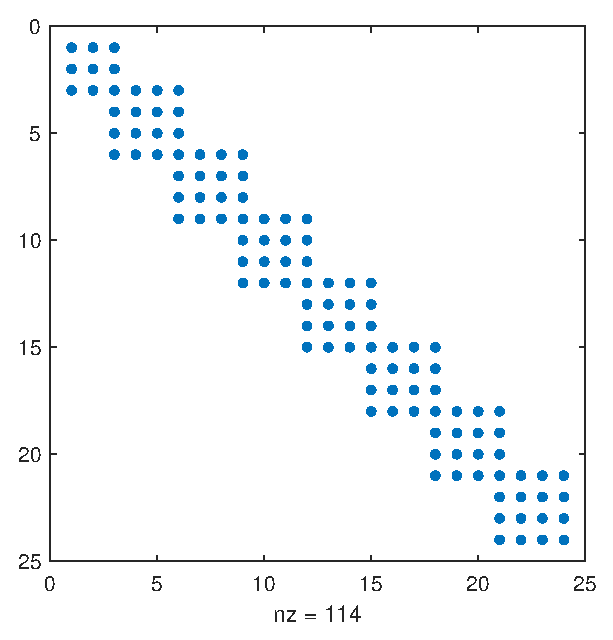
\includegraphics[width=\linewidth]{includefiles/1D poisson LDG spy/lobatto c=05 reduce.eps}
				\caption{\(C_{12} = \frac{1}{2}\), condensed matrix}
			\end{center}
		\end{subfigure}
		\caption{Lobatto nodes, \(k = 2\)，\(N = 8\)}
		\label{1D LDG Lobatto node spy}
	\end{center}
\end{figure}


\subsubsection{Numerical Example (1D Neumann)}

区域 \(\Omega = [0,3\pi]\)，准确解 \(u(x) = \exp\left(\sin(x)\right)\)，采用纯 Neumann 边界条件。空间剖分使用均匀网格，用 \(N\) 表示单元个数，\(k\) 表示多项式次数。取罚参数 \(C_{11} = \eta h^{-\alpha}\)，其中 \(\eta = 1\). 我们使用 Legendre 配点法，使用 Gauss-Legendre 公式进行源项 \(f\) 的数值积分和误差测量。通过添加 Lagrange 乘子\cite{10.1007/BF01436561}，该问题的方程组为：
\begin{equation}
	\begin{aligned}
		& \text{find \(\left(\sigma_{h}, u_{h}, \lambda\right)  \in \Sigma_{h} \times V_{h} \times \R\) such that \(\forall \left(\tau_{h}, v_{h}, \xi\right) \in \Sigma_{h} \times V_{h} \times \R\):} \\
		& \begin{cases}
			a_{h}\left(\sigma_{h}, \tau_h\right) + b_{h}\left(\tau_{h}, u_{h}\right) = F_{h}\left(\tau_{h}\right) \\
			b_{h}\left(\sigma_{h}, v_{h}\right) - c_{h}\left(u_{h}, v_{h}\right) + \left(\lambda, v_{h}\right) = -G_{h}\left(v_{h}\right) \\
			\left(u_{h}, \xi\right) = c_0 \xi
		\end{cases}
	\end{aligned}
\end{equation}
这里，\(c_0\in\R\) 可以任取。为了方便测试精度，我们取
\begin{equation}
	c_0 = \int_{\Omega}u(x)\d x \approx 14.163684556723955471
\end{equation}
测试结果如表所示：

\begin{table}[H]
	\begin{center}
		\resizebox{\linewidth}{!}{
		\begin{tabular}{c | c c | c c | c c | c c }
			\toprule

			\multirow{2}{*}{\(N\)} & \multicolumn{4}{c |}{\(C_{12} = 0\)} & \multicolumn{4}{c}{\(C_{12} = \frac{1}{2}\)} \\
			& \(\norm{u - u_{h}}_{L^2}\) & order & \(\norm{\sigma -\sigma_{h}}_{L^2}\) & order & \(\norm{u - u_{h}}_{L^2}\) & order & \(\norm{\sigma -\sigma_{h}}_{L^2}\) & order \\

			\midrule

			16 & 7.5244e-01 & - & 1.1628e+00 & - & 8.6721e-01 & - & 1.6614e+00 & - \\
			32 & 5.0769e-01 & 0.5676 & 7.1953e-01 & 0.6924 & 5.5180e-01 & 0.6522 & 1.0315e+00 & 0.6877 \\
			64 & 3.0275e-01 & 0.7458 & 4.1635e-01 & 0.7893 & 3.1661e-01 & 0.8014 & 6.2037e-01 & 0.7335 \\
			128 & 1.6670e-01 & 0.8609 & 2.2916e-01 & 0.8614 & 1.7056e-01 & 0.8925 & 3.7476e-01 & 0.7272 \\
			256 & 8.7676e-02 & 0.9270 & 1.2284e-01 & 0.8995 & 8.8667e-02 & 0.9438 & 2.3365e-01 & 0.6816 \\
			512 & 4.4986e-02 & 0.9627 & 6.5290e-02 & 0.9119 & 4.5226e-02 & 0.9712 & 1.5165e-01 & 0.6236 \\

			\bottomrule
		\end{tabular}
		}
		\caption{\(k = 0\)，\(\alpha = 0\)}
	\end{center}
\end{table}

\begin{table}[H]
	\begin{center}
		\resizebox{\linewidth}{!}{
		\begin{tabular}{c | c c | c c | c c | c c }
			\toprule

			\multirow{2}{*}{\(N\)} & \multicolumn{4}{c |}{\(C_{12} = 0\)} & \multicolumn{4}{c}{\(C_{12} = \frac{1}{2}\)} \\
			& \(\norm{u - u_{h}}_{L^2}\) & order & \(\norm{\sigma -\sigma_{h}}_{L^2}\) & order & \(\norm{u - u_{h}}_{L^2}\) & order & \(\norm{\sigma -\sigma_{h}}_{L^2}\) & order \\

			\midrule

			16 & 8.8473e-02 & - & 4.9560e-01 & - & 5.8073e-02 & - & 2.2219e-01 & - \\
			32 & 2.5679e-02 & 1.7846 & 2.9573e-01 & 0.7449 & 1.4372e-02 & 2.0146 & 9.6760e-02 & 1.1993 \\
			64 & 6.7734e-03 & 1.9227 & 1.5975e-01 & 0.8885 & 3.5488e-03 & 2.0179 & 4.4622e-02 & 1.1166 \\
			128 & 1.7195e-03 & 1.9779 & 8.1800e-02 & 0.9656 & 8.8065e-04 & 2.0107 & 2.1429e-02 & 1.0582 \\
			256 & 4.3159e-04 & 1.9943 & 4.1161e-02 & 0.9908 & 2.1930e-04 & 2.0056 & 1.0508e-02 & 1.0281 \\
			512 & 1.0801e-04 & 1.9985 & 2.0614e-02 & 0.9977 & 5.4716e-05 & 2.0029 & 5.2042e-03 & 1.0137 \\

			\bottomrule
		\end{tabular}
		}
		\caption{\(k = 1\)，\(\alpha = -1\)}
	\end{center}
\end{table}

\begin{table}[H]
	\begin{center}
		\resizebox{\linewidth}{!}{
		\begin{tabular}{c | c c | c c | c c | c c }
			\toprule

			\multirow{2}{*}{\(N\)} & \multicolumn{4}{c |}{\(C_{12} = 0\)} & \multicolumn{4}{c}{\(C_{12} = \frac{1}{2}\)} \\
			& \(\norm{u - u_{h}}_{L^2}\) & order & \(\norm{\sigma -\sigma_{h}}_{L^2}\) & order & \(\norm{u - u_{h}}_{L^2}\) & order & \(\norm{\sigma -\sigma_{h}}_{L^2}\) & order \\

			\midrule

			16 & 2.7178e-03 & - & 1.6452e-02 & - & 4.4262e-03 & - & 2.1686e-02 & - \\
			32 & 1.8862e-04 & 3.8489 & 3.7120e-03 & 2.1480 & 5.5809e-04 & 2.9875 & 4.0348e-03 & 2.4262 \\
			64 & 1.9064e-05 & 3.3065 & 9.2275e-04 & 2.0082 & 7.0006e-05 & 2.9949 & 9.4059e-04 & 2.1009 \\
			128 & 2.2391e-06 & 3.0899 & 2.3050e-04 & 2.0012 & 8.7594e-06 & 2.9986 & 2.3154e-04 & 2.0223 \\
			256 & 2.7534e-07 & 3.0236 & 5.7616e-05 & 2.0002 & 1.0952e-06 & 2.9996 & 5.7678e-05 & 2.0052 \\
			512 & 3.4276e-08 & 3.0060 & 1.4403e-05 & 2.0001 & 1.3691e-07 & 2.9999 & 1.4407e-05 & 2.0012 \\

			\bottomrule
		\end{tabular}
		}
		\caption{\(k = 2\)，\(\alpha = -1\)}
	\end{center}
\end{table}

\begin{table}[H]
	\begin{center}
		\resizebox{\linewidth}{!}{
		\begin{tabular}{c | c c | c c | c c | c c }
			\toprule

			\multirow{2}{*}{\(N\)} & \multicolumn{4}{c |}{\(C_{12} = 0\)} & \multicolumn{4}{c}{\(C_{12} = \frac{1}{2}\)} \\
			& \(\norm{u - u_{h}}_{L^2}\) & order & \(\norm{\sigma -\sigma_{h}}_{L^2}\) & order & \(\norm{u - u_{h}}_{L^2}\) & order & \(\norm{\sigma -\sigma_{h}}_{L^2}\) & order \\

			\midrule

			16 & 4.0148e-04 & - & 3.5596e-03 & - & 3.5424e-04 & - & 2.9273e-03 & - \\
			32 & 3.2820e-05 & 3.6127 & 7.4574e-04 & 2.2550 & 2.2188e-05 & 3.9969 & 2.4151e-04 & 3.5994 \\
			64 & 2.0681e-06 & 3.9882 & 1.2565e-04 & 2.5693 & 1.3864e-06 & 4.0004 & 2.3403e-05 & 3.3673 \\
			128 & 1.2134e-07 & 4.0911 & 1.7659e-05 & 2.8309 & 8.6598e-08 & 4.0009 & 2.5830e-06 & 3.1796 \\
			256 & 7.3211e-09 & 4.0509 & 2.2876e-06 & 2.9485 & 5.4100e-09 & 4.0006 & 3.0493e-07 & 3.0825 \\
			512 & 4.5245e-10 & 4.0162 & 2.8869e-07 & 2.9863 & 3.3808e-10 & 4.0002 & 3.7117e-08 & 3.0383 \\

			\bottomrule
		\end{tabular}
		}
		\caption{\(k = 3\)，\(\alpha = -1\)}
	\end{center}
\end{table}

\begin{table}[H]
	\begin{center}
		\resizebox{\linewidth}{!}{
		\begin{tabular}{c | c c | c c | c c | c c }
			\toprule

			\multirow{2}{*}{\(N\)} & \multicolumn{4}{c |}{\(C_{12} = 0\)} & \multicolumn{4}{c}{\(C_{12} = \frac{1}{2}\)} \\
			& \(\norm{u - u_{h}}_{L^2}\) & order & \(\norm{\sigma -\sigma_{h}}_{L^2}\) & order & \(\norm{u - u_{h}}_{L^2}\) & order & \(\norm{\sigma -\sigma_{h}}_{L^2}\) & order \\

			\midrule

			16 & 2.9801e-05 & - & 1.7023e-04 & - & 2.5638e-05 & - & 1.5584e-04 & - \\
			32 & 3.6205e-07 & 6.3630 & 6.4132e-06 & 4.7303 & 8.2181e-07 & 4.9634 & 8.7328e-06 & 4.1575 \\
			64 & 6.3533e-09 & 5.8325 & 3.7029e-07 & 4.1143 & 2.5794e-08 & 4.9937 & 4.5827e-07 & 4.2522 \\
			128 & 1.3893e-10 & 5.5150 & 2.2412e-08 & 4.0463 & 8.0651e-10 & 4.9992 & 2.5304e-08 & 4.1788 \\
			256 & 4.2896e-12 & 5.0174 & 1.3792e-09 & 4.0224 & 2.5282e-11 & 4.9955 & 1.4710e-09 & 4.1045 \\
			512 & 2.1149e-12 & 1.0202 & 8.5533e-11 & 4.0112 & 5.0409e-12 & 2.3264 & 8.8439e-11 & 4.0560 \\

			\bottomrule
		\end{tabular}
		}
		\caption{\(k = 4\)，\(\alpha = -1\)}
	\end{center}
\end{table}


\subsubsection{Numerical Example (2D Dirichlet)}

取多边形区域 \(\Omega = \B{(x,y) \big| -1\leqslant x, y \leqslant 1, y-x+1\geqslant 0}\)，取准确解 \(u(x, y) = \exp\left(\sin(\pi x)\right)\cos(\pi(x + y))\)，采用 Dirichlet 边界条件。

我们采用 MD-LDG 方法\cite{10.1007/s10915-007-9130-3}：在 Dirichlet 边界上 \(C_{11} = \eta h_{\perp}^{-\alpha}\)，其中 \(\eta = 10\)，\(\alpha = -1\)，\(h_{\perp}\) 是三角形中边对应的高；在其余边上 \(C_{11} = 0\)；在内部边上 \(\bm C_{12}(e) = \frac{\bm n_{e}}{2} {\rm sgn}\left(\int_{e} \bm v_0\cdot\bm n_{e} \d s\right)\) (边界上 \(\bm C_{12}\) 无定义)，这里 \(\bm v_0 \in H({\rm div}, \Omega)^{d}\).

我们使用 Nodal DG 方法实现，在三角形单元上使用如图\ref{P6 Lobatto nodes}的 Lobatto 配点集，并使用该配点集上的多项式插值计算积分，编写了支持协调三角网格上任意高阶多项式的 Matlab 程序，具体的矩阵组装过程、技巧以及数据结构参考文章\cite{10.1016/j.camwa.2015.04.013}。我们使用开源软件 gmsh 画网格，在本算例中采用了如图\ref{Mesh: 2D Dirichlet}的二等分逐层加密的三角网格。组装的矩阵的稀疏模式如图\ref{2D MD-LDG Lobatto node spy}所示，这里 \(k\) 表示多项式次数。由于原始方程组规模较大，我们使用 Schur 补\eqref{LDG Schur complement}以减小规模。值得一提的是，由于我们使用的是 Lobatto 配点，可以区分单元内部和边界自由度，因此可以使用逐单元的 static condensation 进一步减小方程组规模，但由于其编程的复杂性，这里并未采用此方法。测试结果如下面的图表所示，其中，\(N_{\rm dof}^{\rm Schur}\) 是使用 Schur 补后的自由度个数，原本的总自由度个数应当是 \(3 N_{\rm dof}^{\rm Schur}\).


% to be done: 具体写一下如何组装的(包括 A，B，C三个矩阵和右端项，如何构造 nodal 基函数等等)，接着 2D Case 那一节写。



\begin{figure}[htbp]
	\begin{center}
		\begin{subfigure}{0.49\linewidth}
			\begin{center}
				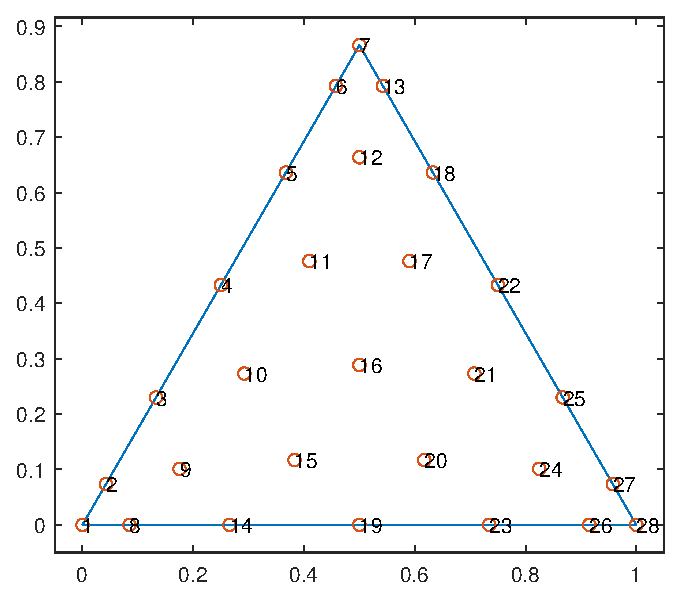
\includegraphics[width=0.8\linewidth]{includefiles/2D poisson LDG/Lobatto2D_equi p6.eps}
				\caption{正三角形单元}
			\end{center}
		\end{subfigure}
		\begin{subfigure}{0.49\linewidth}
			\begin{center}
				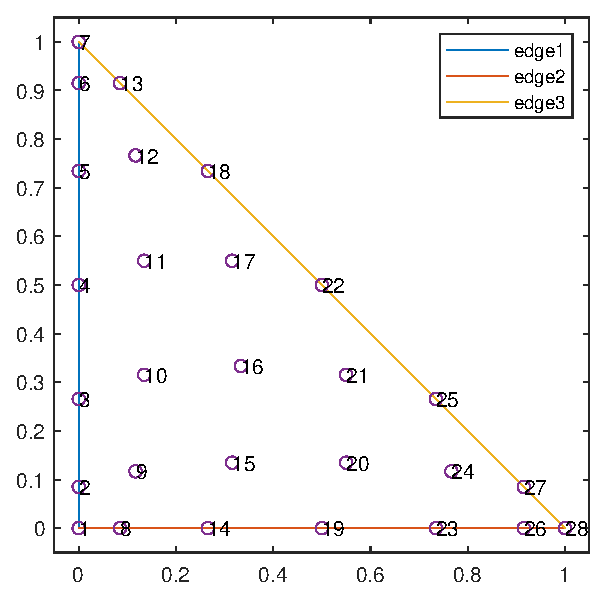
\includegraphics[width=0.8\linewidth]{includefiles/2D poisson LDG/Lobatto2D_ref p6.eps}
				\caption{三角形参考单元}
			\end{center}
		\end{subfigure}
		\caption{\(\mathscr{P}^{6}\) Lobatto 配点集及自由度排序}
		\label{P6 Lobatto nodes}
	\end{center}
\end{figure}

\begin{figure}[htbp]
	\begin{center}
		\begin{subfigure}{0.32\linewidth}
			\begin{center}
				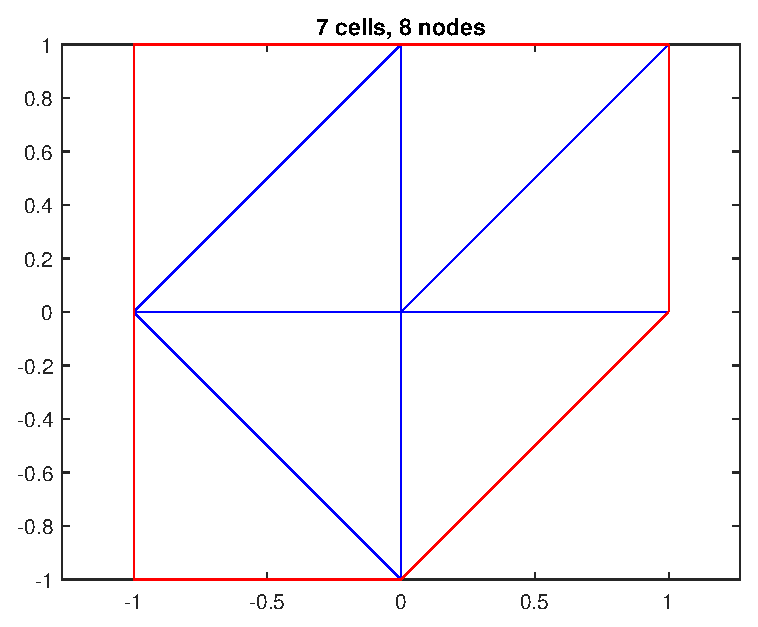
\includegraphics[width=\linewidth]{includefiles/2D poisson LDG/mesh1.eps}
				\caption{mesh 1}
			\end{center}
		\end{subfigure}
		\begin{subfigure}{0.32\linewidth}
			\begin{center}
				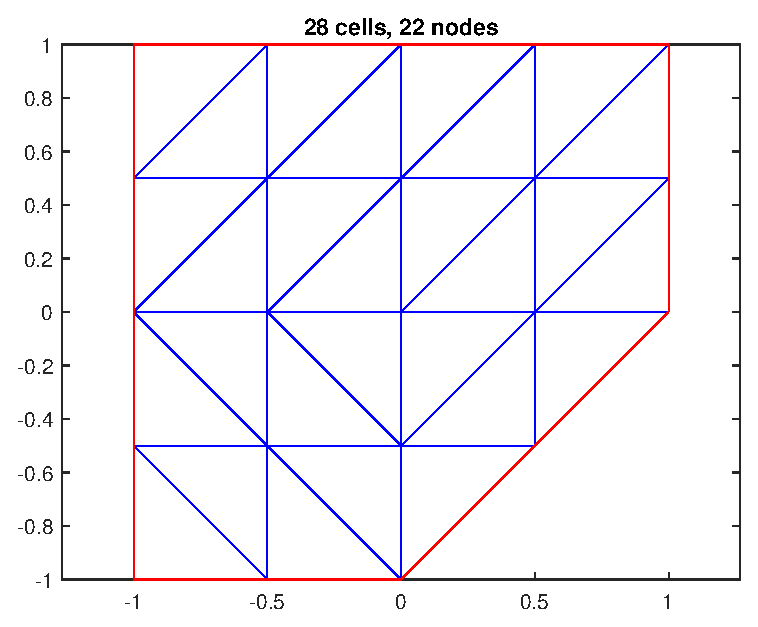
\includegraphics[width=\linewidth]{includefiles/2D poisson LDG/mesh2.eps}
				\caption{mesh 2}
			\end{center}
		\end{subfigure}
		\begin{subfigure}{0.32\linewidth}
			\begin{center}
				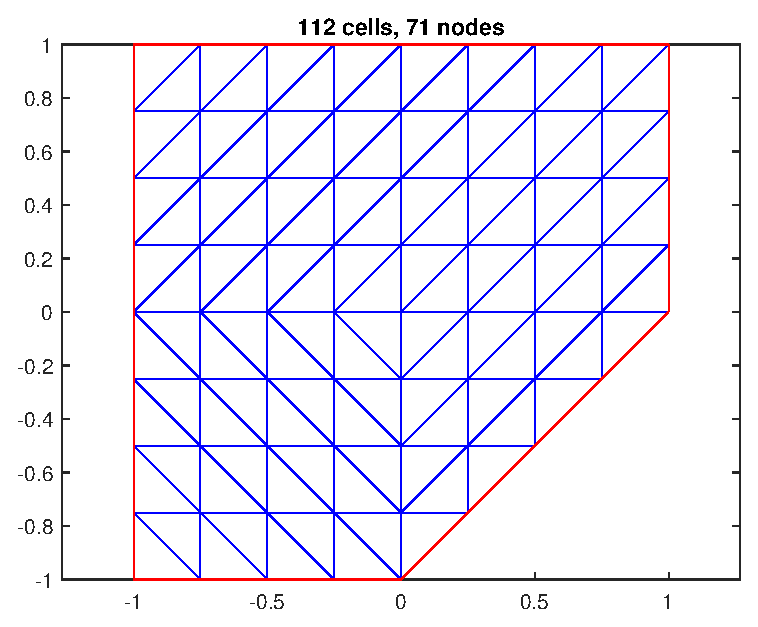
\includegraphics[width=\linewidth]{includefiles/2D poisson LDG/mesh3.eps}
				\caption{mesh 3}
			\end{center}
		\end{subfigure}

		\begin{subfigure}{0.32\linewidth}
			\begin{center}
				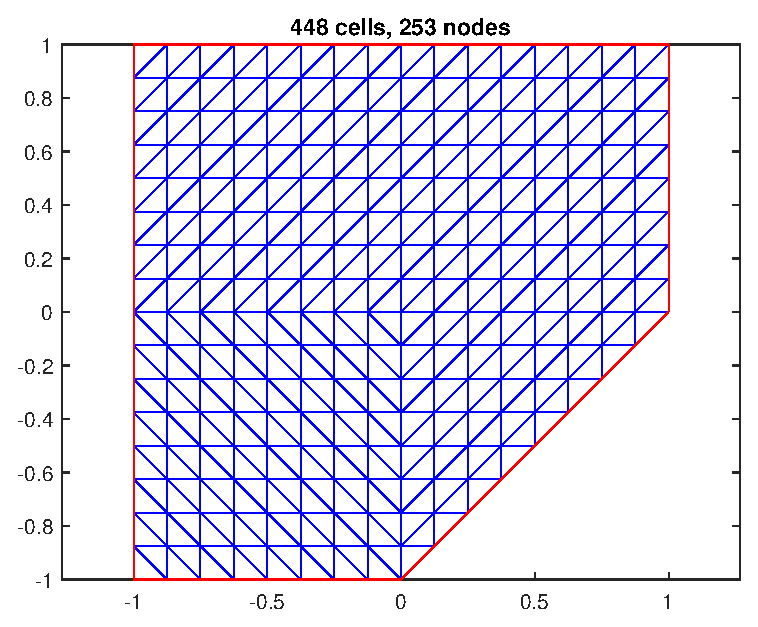
\includegraphics[width=\linewidth]{includefiles/2D poisson LDG/mesh4.eps}
				\caption{mesh 4}
			\end{center}
		\end{subfigure}
		\begin{subfigure}{0.32\linewidth}
			\begin{center}
				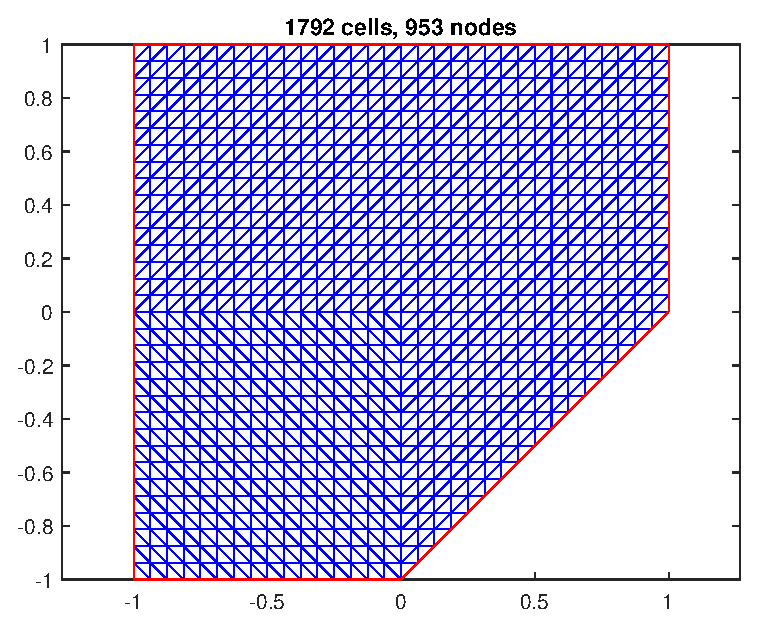
\includegraphics[width=\linewidth]{includefiles/2D poisson LDG/mesh5.eps}
				\caption{mesh 5}
			\end{center}
		\end{subfigure}
		\begin{subfigure}{0.32\linewidth}
			\begin{center}
				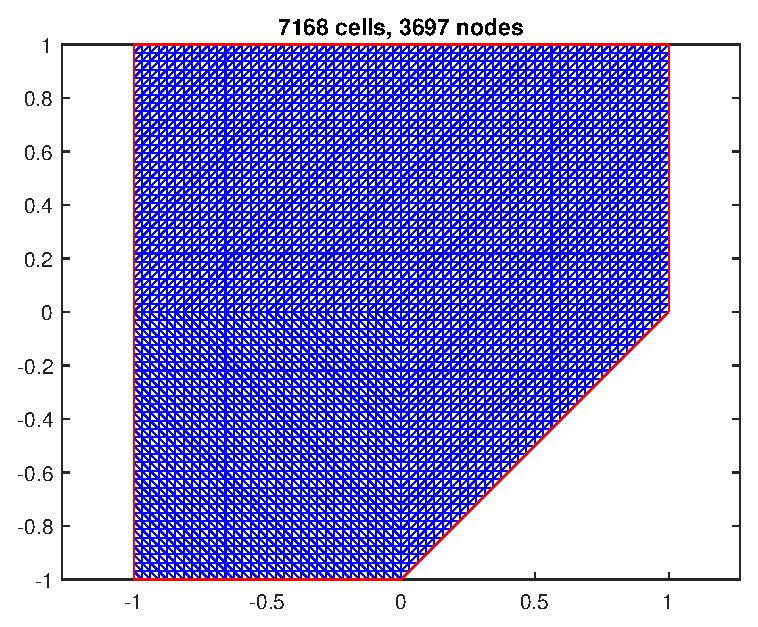
\includegraphics[width=\linewidth]{includefiles/2D poisson LDG/mesh6.eps}
				\caption{mesh 6}
			\end{center}
		\end{subfigure}
		\caption{算例使用的网格}
		\label{Mesh: 2D Dirichlet}
	\end{center}
\end{figure}

\begin{figure}[htbp]
	\begin{center}
		\begin{subfigure}{0.49\linewidth}
			\begin{center}
				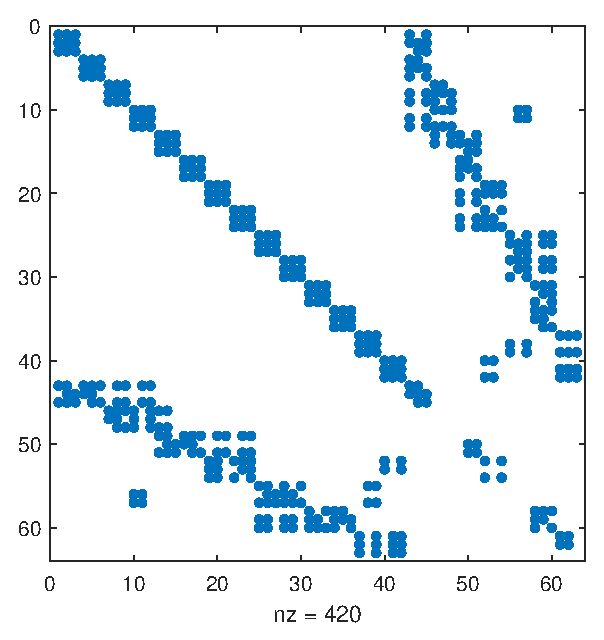
\includegraphics[width=0.8\linewidth]{includefiles/2D poisson LDG/spyZZ p1.eps}
				\caption{original matrix, \(k=1\)}
			\end{center}
		\end{subfigure}
		\begin{subfigure}{0.49\linewidth}
			\begin{center}
				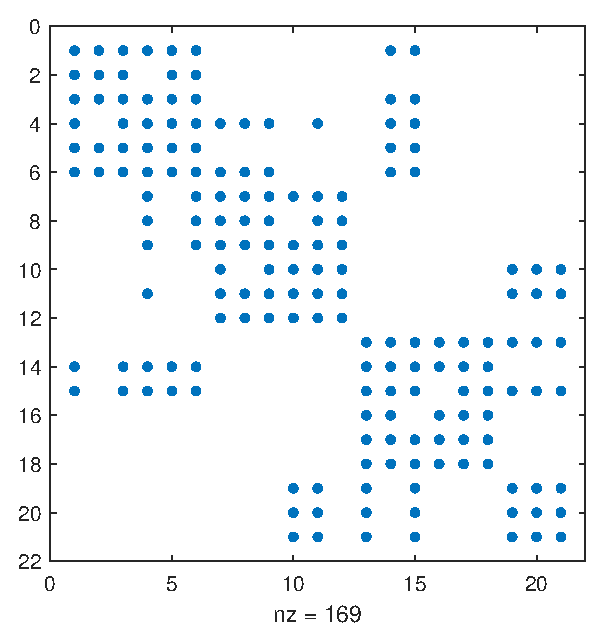
\includegraphics[width=0.8\linewidth]{includefiles/2D poisson LDG/spySS p1.eps}
				\caption{condensed matrix, \(k=1\)}
			\end{center}
		\end{subfigure}

		\begin{subfigure}{0.49\linewidth}
			\begin{center}
				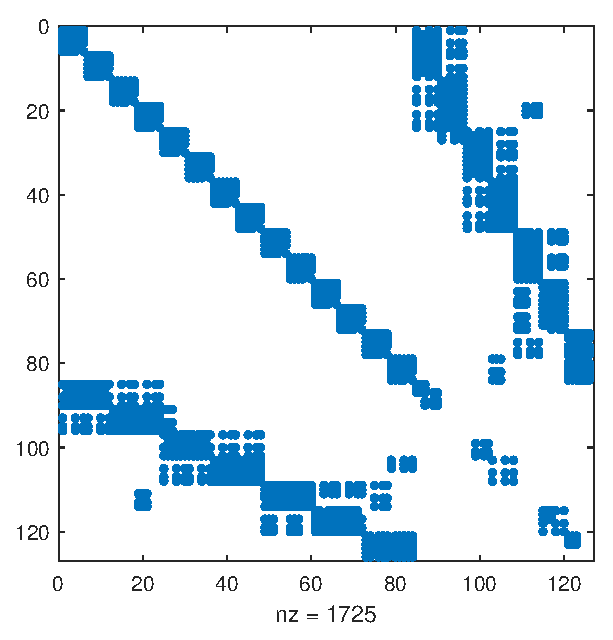
\includegraphics[width=0.8\linewidth]{includefiles/2D poisson LDG/spyZZ p2.eps}
				\caption{original matrix, \(k=2\)}
			\end{center}
		\end{subfigure}
		\begin{subfigure}{0.49\linewidth}
			\begin{center}
				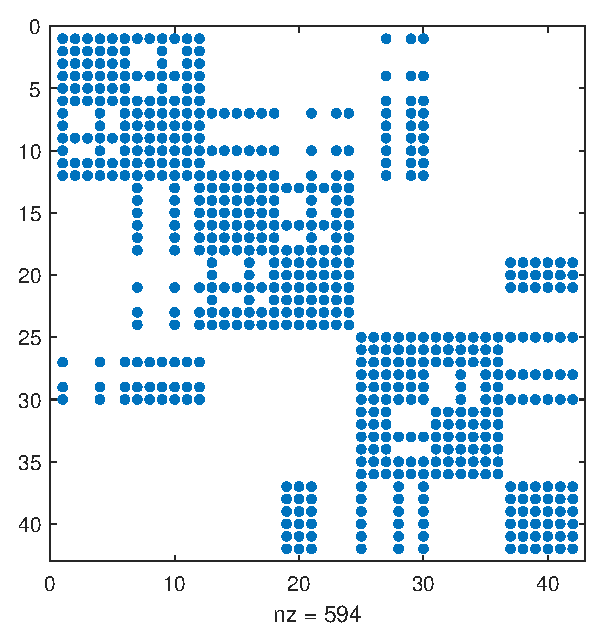
\includegraphics[width=0.8\linewidth]{includefiles/2D poisson LDG/spySS p2.eps}
				\caption{condensed matrix, \(k=2\)}
			\end{center}
		\end{subfigure}

		\begin{subfigure}{0.49\linewidth}
			\begin{center}
				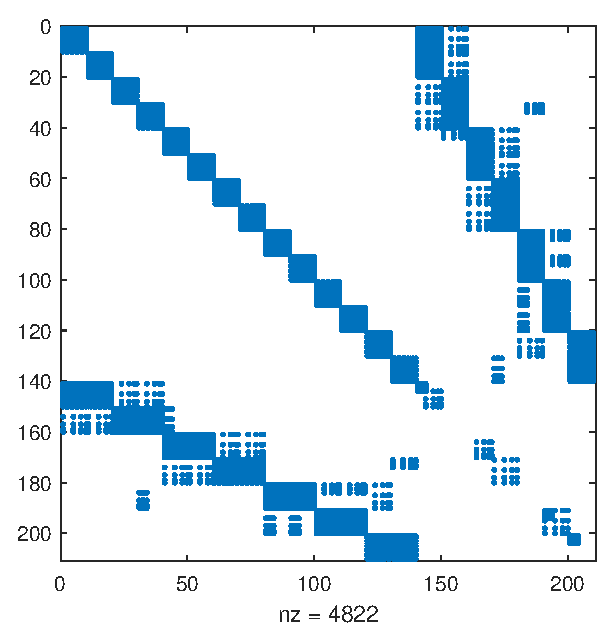
\includegraphics[width=0.8\linewidth]{includefiles/2D poisson LDG/spyZZ p3.eps}
				\caption{original matrix, \(k=3\)}
			\end{center}
		\end{subfigure}
		\begin{subfigure}{0.49\linewidth}
			\begin{center}
				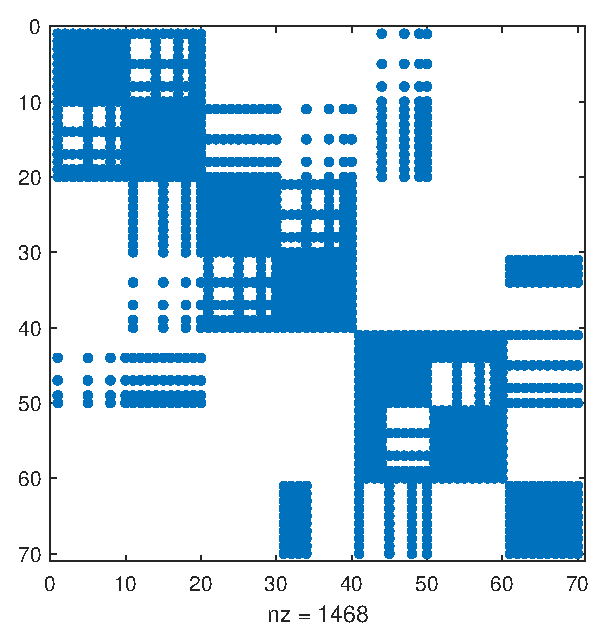
\includegraphics[width=0.8\linewidth]{includefiles/2D poisson LDG/spySS p3.eps}
				\caption{condensed matrix, \(k=3\)}
			\end{center}
		\end{subfigure}
		\caption{sparsity patterns on the coarsest mesh}
		\label{2D MD-LDG Lobatto node spy}
	\end{center}
\end{figure}

\begin{figure}[htbp]
	\begin{center}
		\begin{subfigure}{0.49\linewidth}
			\begin{center}
				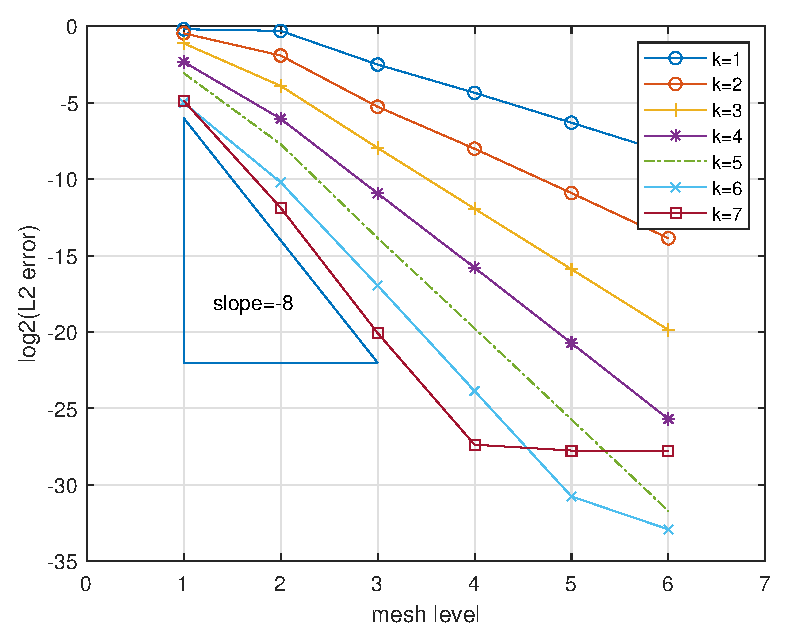
\includegraphics[width=\linewidth]{includefiles/2D poisson LDG/error_u.eps}
				\caption{\(u\)}
			\end{center}
		\end{subfigure}
		\begin{subfigure}{0.49\linewidth}
			\begin{center}
				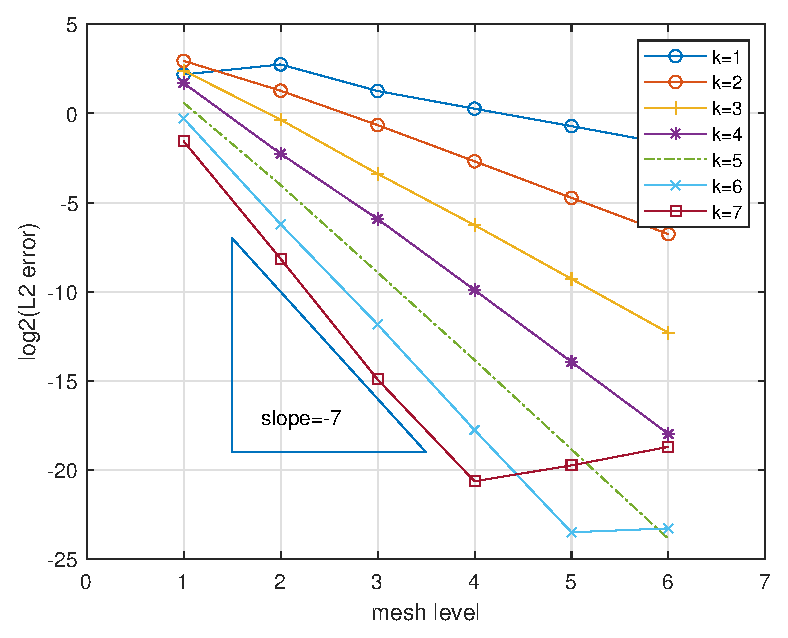
\includegraphics[width=\linewidth]{includefiles/2D poisson LDG/error_q.eps}
				\caption{\(\sigma\)}
			\end{center}
		\end{subfigure}
		\caption{convergence with different \(k\)}
	\end{center}
\end{figure}


\begin{table}[H]
	\begin{center}
		\begin{tabular}{ c c | c c | c c }
			\toprule

			\(N_{e}\) & \(N_{\rm dof}^{\rm Schur}\) & \(\norm{u - u_{h}}_{L^2}\) & order & \(\norm{\sigma -\sigma_{h}}_{L^2}\) & order \\

			\midrule

			7 & 21 & 8.7226e-01 & - & 4.5397e+00 & -  \\
			28 & 84 & 8.1148e-01 & 0.1042 & 6.7114e+00 & -0.5640 \\
			112 & 336 & 1.7621e-01 & 2.2032 & 2.3930e+00 & 1.4878 \\
			448 & 1344 & 4.8970e-02 & 1.8473 & 1.2005e+00 & 0.9952 \\
			1792 & 5376 & 1.2598e-02 & 1.9587 & 6.1048e-01 & 0.9756 \\
			7168 & 21504 & 3.1675e-03 & 1.9917 & 3.0435e-01 & 1.0042 \\

			\bottomrule
		\end{tabular}
		\caption{\(k = 1\)}
	\end{center}
\end{table}

\begin{table}[H]
	\begin{center}
		\begin{tabular}{ c c | c c | c c }
			\toprule

			\(N_{e}\) & \(N_{\rm dof}^{\rm Schur}\) & \(\norm{u - u_{h}}_{L^2}\) & order & \(\norm{\sigma -\sigma_{h}}_{L^2}\) & order \\

			\midrule

			7 & 42 & 7.2670e-01 & - & 7.7261e+00 & -  \\
			28 & 168 & 2.6543e-01 & 1.4530 & 2.4176e+00 & 1.6761 \\
			112 & 672 & 2.6000e-02 & 3.3518 & 6.3527e-01 & 1.9282 \\
			448 & 2688 & 3.8776e-03 & 2.7453 & 1.5561e-01 & 2.0294 \\
			1792 & 10752 & 5.1788e-04 & 2.9045 & 3.7654e-02 & 2.0471 \\
			7168 & 43008 & 6.6718e-05 & 2.9565 & 9.1440e-03 & 2.0419 \\

			\bottomrule
		\end{tabular}
		\caption{\(k = 2\)}
	\end{center}
\end{table}

\begin{table}[H]
	\begin{center}
		\begin{tabular}{ c c | c c | c c }
			\toprule

			\(N_{e}\) & \(N_{\rm dof}^{\rm Schur}\) & \(\norm{u - u_{h}}_{L^2}\) & order & \(\norm{\sigma -\sigma_{h}}_{L^2}\) & order \\

			\midrule

			7 & 70 & 4.6247e-01 & - & 5.2916e+00 & - \\
			28 & 280 & 6.6979e-02 & 2.7876 & 7.8343e-01 & 2.7558 \\
			112 & 1120 & 4.0264e-03 & 4.0561 & 9.5777e-02 & 3.0320 \\
			448 & 4480 & 2.5512e-04 & 3.9802 & 1.3018e-02 & 2.8792 \\
			1792 & 17920 & 1.6386e-05 & 3.9606 & 1.6076e-03 & 3.0175 \\
			7168 & 71680 & 1.0441e-06 & 3.9722 & 1.9770e-04 & 3.0235 \\

			\bottomrule
		\end{tabular}
		\caption{\(k = 3\)}
	\end{center}
\end{table}

\begin{table}[H]
	\begin{center}
		\begin{tabular}{ c c | c c | c c }
			\toprule

			\(N_{e}\) & \(N_{\rm dof}^{\rm Schur}\) & \(\norm{u - u_{h}}_{L^2}\) & order & \(\norm{\sigma -\sigma_{h}}_{L^2}\) & order \\

			\midrule

			7 & 105 & 1.9892e-01 & - & 3.2592e+00 & - \\
			28 & 420 & 1.5130e-02 & 3.7167 & 2.0889e-01 & 3.9637 \\
			112 & 1680 & 5.1190e-04 & 4.8854 & 1.6561e-02 & 3.6568 \\
			448 & 6720 & 1.7635e-05 & 4.8593 & 1.0465e-03 & 3.9842 \\
			1792 & 26880 & 5.7470e-07 & 4.9395 & 6.3816e-05 & 4.0355 \\
			7168 & 107520 & 1.8310e-08 & 4.9721 & 3.8879e-06 & 4.0368 \\

			\bottomrule
		\end{tabular}
		\caption{\(k = 4\)}
	\end{center}
\end{table}

\begin{table}[H]
	\begin{center}
		\begin{tabular}{ c c | c c | c c }
			\toprule

			\(N_{e}\) & \(N_{\rm dof}^{\rm Schur}\) & \(\norm{u - u_{h}}_{L^2}\) & order & \(\norm{\sigma -\sigma_{h}}_{L^2}\) & order \\

			\midrule

			7 & 147 & 1.1964e-01 & - & 1.5125e+00 & - \\
			28 & 588 & 4.7762e-03 & 4.6467 & 6.1947e-02 & 4.6098 \\
			112 & 2352 & 6.7727e-05 & 6.1400 & 2.0665e-03 & 4.9058 \\
			448 & 9408 & 1.1245e-06 & 5.9124 & 6.8727e-05 & 4.9101 \\
			1792 & 37632 & 1.7977e-08 & 5.9670 & 2.1323e-06 & 5.0104 \\
			7168 & 150528 & 2.8382e-10 & 5.9850 & 6.5653e-08 & 5.0214 \\

			\bottomrule
		\end{tabular}
		\caption{\(k = 5\)}
	\end{center}
\end{table}

\begin{table}[H]
	\begin{center}
		\begin{tabular}{ c c | c c | c c }
			\toprule

			\(N_{e}\) & \(N_{\rm dof}^{\rm Schur}\) & \(\norm{u - u_{h}}_{L^2}\) & order & \(\norm{\sigma -\sigma_{h}}_{L^2}\) & order \\

			\midrule

			7 & 196 & 3.1120e-02 & - & 8.2439e-01 & - \\
			28 & 784 & 8.4563e-04 & 5.2017 & 1.3474e-02 & 5.9351 \\
			112 & 3136 & 7.8587e-06 & 6.7496 & 2.7488e-04 & 5.6152 \\
			448 & 12544 & 6.6028e-08 & 6.8951 & 4.5426e-06 & 5.9191 \\
			1792 & 50176 & 5.4896e-10 & 6.9102 & 8.5027e-08 & 5.7395 \\
			7168 & 200704 & 1.2334e-10 & 2.1541 & 9.8961e-08 & -0.2189 \\

			\bottomrule
		\end{tabular}
		\caption{\(k = 6\)}
	\end{center}
\end{table}

\begin{table}[H]
	\begin{center}
		\begin{tabular}{ c c | c c | c c }
			\toprule

			\(N_{e}\) & \(N_{\rm dof}^{\rm Schur}\) & \(\norm{u - u_{h}}_{L^2}\) & order & \(\norm{\sigma -\sigma_{h}}_{L^2}\) & order \\

			\midrule

			7 & 252 & 3.4188e-02 & - & 3.4023e-01 & - \\
			28 & 1008 & 2.6723e-04 & 6.9992 & 3.5253e-03 & 6.5926 \\
			112 & 4032 & 9.1421e-07 & 8.1913 & 3.2384e-05 & 6.7663 \\
			448 & 16128 & 5.7531e-09 & 7.3120 & 6.1755e-07 & 5.7126 \\
			1792 & 64512 & 4.4026e-09 & 0.3860 & 1.1468e-06 & -0.8929 \\
			7168 & 258048 & 4.4031e-09 & -0.0002 & 2.3527e-06 & -1.0368 \\

			\bottomrule
		\end{tabular}
		\caption{\(k = 7\)}
	\end{center}
\end{table}

% 注记：几乎全部的计算时间都在组装矩阵上了(通过我重写程序中的边界积分，时间迅速下降了，例如k=6的最密网格，时间从640秒缩到7.5秒)；使用 Schur 补会提高数值精度，且可以加速计算(k=7最密网格，使用Schur补的直接解法需要4.3秒，原本解法需要28.6秒)

\iffalse
% k=7结果：
assembly time = 0.035459 s, solving time = 0.008535, NDOF = 756 
assembly time = 0.066276 s, solving time = 0.032241, NDOF = 3024 
assembly time = 0.132961 s, solving time = 0.144986, NDOF = 12096 
assembly time = 0.447437 s, solving time = 0.638908, NDOF = 48384 
assembly time = 4.411273 s, solving time = 4.496390, NDOF = 193536 
assembly time = 44.004316 s, solving time = 27.028705, NDOF = 774144 

% 误差表：
k=1:
8.7226e-01   4.5397e+00
8.1148e-01   6.7114e+00
1.7621e-01   2.3930e+00
4.8970e-02   1.2005e+00
1.2598e-02   6.1048e-01
3.1675e-03   3.0435e-01

k=2:
7.2670e-01   7.7261e+00
2.6543e-01   2.4176e+00
2.6000e-02   6.3527e-01
3.8776e-03   1.5561e-01
5.1788e-04   3.7654e-02
6.6718e-05   9.1440e-03

k=3:
4.6247e-01   5.2916e+00
6.6979e-02   7.8343e-01
4.0264e-03   9.5777e-02
2.5512e-04   1.3018e-02
1.6386e-05   1.6076e-03
1.0441e-06   1.9770e-04

k=4:
1.9892e-01   3.2592e+00
1.5130e-02   2.0889e-01
5.1190e-04   1.6561e-02
1.7635e-05   1.0465e-03
5.7470e-07   6.3816e-05
1.8310e-08   3.8879e-06

k=5:
1.1964e-01   1.5125e+00
4.7762e-03   6.1947e-02
6.7727e-05   2.0665e-03
1.1245e-06   6.8727e-05
1.7977e-08   2.1323e-06
2.8382e-10   6.5653e-08

k=6:
3.1120e-02   8.2439e-01
8.4563e-04   1.3474e-02
7.8587e-06   2.7488e-04
6.6028e-08   4.5426e-06
5.4896e-10   8.5027e-08
1.2334e-10   9.8961e-08

k=7:
3.4188e-02   3.4023e-01
2.6723e-04   3.5253e-03
9.1421e-07   3.2384e-05
5.7531e-09   6.1755e-07
4.4026e-09   1.1468e-06
4.4031e-09   2.3527e-06

绘图：
plot(1:6,log2(err(:,1,1)), '-o');
hold on;
plot(1:6,log2(err(:,1,2)), '-o');
hold on;
plot(1:6,log2(err(:,1,3)), '-+');
hold on;
plot(1:6,log2(err(:,1,4)), '-*');
hold on;
plot(1:6,log2(err(:,1,5)), '-.');
hold on;
plot(1:6,log2(err(:,1,6)), '-x');
hold on;
plot(1:6,log2(err(:,1,7)), '-s');
hold on;
plot([1, 3, 1, 1], [-22, -22, -6, -22]);
hold on;
text(1.3,-18,'slope=-8');
grid on;
legend('k=1','k=2','k=3','k=4','k=5','k=6', 'k=7');
xlabel('mesh level');
ylabel('log2(L2 error)');
xlim([0,7]);
hold off;
print(gcf, '-depsc2', '-vector', 'error_u', '-r300');

plot(1:6,log2(err(:,2,1)), '-o');
hold on;
plot(1:6,log2(err(:,2,2)), '-o');
hold on;
plot(1:6,log2(err(:,2,3)), '-+');
hold on;
plot(1:6,log2(err(:,2,4)), '-*');
hold on;
plot(1:6,log2(err(:,2,5)), '-.');
hold on;
plot(1:6,log2(err(:,2,6)), '-x');
hold on;
plot(1:6,log2(err(:,2,7)), '-s');
hold on;
plot([1.5, 3.5, 1.5, 1.5], [-19, -19, -7, -19]);
hold on;
text(1.8,-17,'slope=-7');
grid on;
legend('k=1','k=2','k=3','k=4','k=5','k=6','k=7');
xlabel('mesh level');
ylabel('log2(L2 error)');
xlim([0,7]);
hold off;
print(gcf, '-depsc2', '-vector', 'error_q', '-r300');
\fi

\subsubsection{Conclusion}

我们编程实现了一维和二维 Poisson 方程的 LDG 方法，该方法的特性是可以由 \(u_{h}\) 和 \(g_{D}\) 局部、显式地表示 \(\sigma_{h}\)，从而可以利用 Schur 补的技巧，减少全局相互耦合的方程组自由度个数，且 Schur 补对应的代数方程组正好是 LDG 框架下 Poisson 方程的 primal 形式。我们的测试显示出对 \((\sigma, u)\) 的 \((k, k+1)\) 阶收敛，与理论结果一致。





\subsection{The Hybridizable DG Method}

%由CG到DG/FV到HDG的介绍：

%The concept of Standard (Continuous Galerkin) Finite Element Methods (CG FEM) is based upon the variational formulation of the PDE. An approximation to the PDE is achieved by replacing the infinite dimensional space in which the variational formulation is posed by a finite dimensional subspace which normally uses (element-) piecewise polynomials which are continuous across element interfaces. This allows for increasing the order of approximation quite easily also on unstructured meshes as only the polynomial degree has to be increased (given that the solution is sufficiently smooth). However, the CG FEM suffers from stability issues for convection-dominated flows and the lack of a conservation property. Finite Volume Methods (FVM) on the other hand, which are frequently used in engineering practice and are build upon the balance of in- and outfluxes on a control volumes, have neither of these problems. But here the problem is that providing higher order approximations with Finite Volume Methods is hardly possible.

%A modern approach which combines the features and overcomes the draw-backs of both methods is the use of Discontinuous Galerkin Finite Element Methods (DG FEM). It is also based upon a variational formulation but this time the finite dimensional space is not taken to be a subspace of the infinite one. Instead, the finite one uses discontinuous functions, which are not allowed in the continuous setting. As the DG FEM approximation with piecewise constant functions coincides with the use of a Finite Volume Method the Finite Volume method is, in a sense, a subclass and thereby its conservation property can be inherited to the DG FEM. Although all stated problems of FVM and CG FEM can be solved with DG FEM, DG FEM has one (big) disadvantage: It introduces considerably more unknowns as CG FEM or FVM. Especially linear systems arising from discretizations with DG FEM are considerably larger and less sparse as a lot of couplings between unknowns of different elements are introduced.


\subsubsection{The HDG Formulation}

HDG 格式利用类似 static condensation\cite{10.2514/3.2874}的思想，将单元边界上的数值通量作为未知量，可以大大缩减求解方程组的规模，并由于其对 \(\left(\sigma, u\right)\) 的一致最优误差阶和超收敛性质，同精度的求解开销可以被进一步降低。实际应用中，在采用直接法求解方程组时，HDG 比 CG-H(使用 static condensation 的CG)有明显优势；在采用迭代法求解时，HDG 对比 CG-H 没有明显优势，这说明 HDG 仍需要更有效的预处理器\cite{10.1007/s10915-015-0076-6}。

\begin{figure}[htbp]
	\begin{center}
		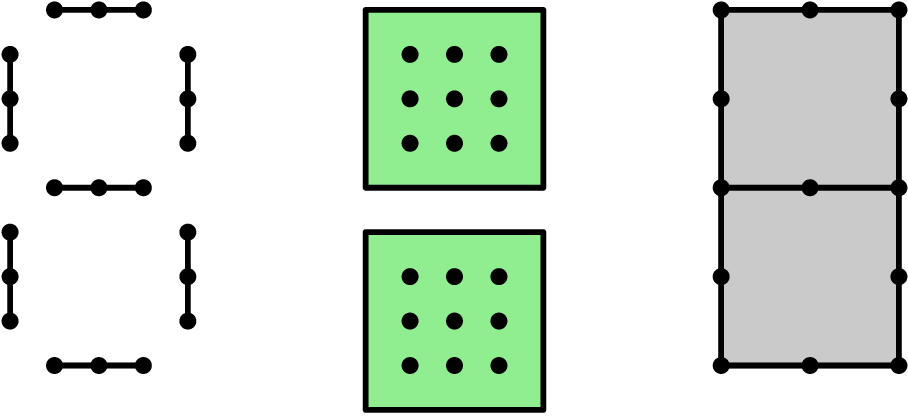
\includegraphics[width=0.8\linewidth]{includefiles/DOF compare.png}
		\caption{DOFs of \(\mathscr{Q}^{2}\) HDG, DG, and CG-H elements\cite{10.48550/arXiv.1705.09907, 10.1137/17M1128903}}
	\end{center}
\end{figure}

我们这里只考虑 LDG-H 格式\cite{10.1137/070706616, 10.1137/080728810}，其他 HDG 格式例如 IP-H 也是类似的。

LDG-H 是守恒的格式(数值通量无跳跃)，把 \(\widehat{u}_{h}\big|_{\Gamma}\) 也作为变量，并限制其满足 Dirichlet 边界条件(强制施加)：
\begin{equation}
	\widehat{u}_{h}\big|_{\Gamma^{D}} = g_{D}
\end{equation}
类似 LDG 格式，令 \(\widehat{\sigma}_{h}\) 具有形式 (\(\tau_{K}\) 在 \(K\) 的每一条边上是非负常数)：
\begin{equation}
	\widehat{\sigma}_{h} = \sigma_{K} - \tau_{K} \left(u_{K} - \widehat{u}_{h}\right) n_{K}
\end{equation}
由于格式守恒，令 \(\widehat{\sigma}_{h}\) 也满足无跳跃条件(该条件在计算中弱施加)：
\begin{equation}
	\begin{cases}
		\widehat{\sigma}_{h}\cdot n\big|_{e} = \bm g_{N}\cdot\bm n , & e\in\mathcal{E}^{N}_{h} \\
		\jump{\widehat{\sigma}_{h}}\big|_{e} = 0, & e \in \mathcal{E}_{h}^{o}
	\end{cases}
\end{equation}
这样，可以将数值通量写成如下形式(仅用于分析，不在计算中直接使用)：
\begin{subequations}\label{LDG-H numerical flux}
	\begin{eqnarray}
		&& \widehat{\sigma}_{h}\big|_{e} = \begin{cases}
			\avg{\sigma_{h}} - \bm C_{12} \jump{\sigma_{h}} - C_{11} \jump{u_{h}}, & e \in \mathcal{E}_{h}^{o} \\
			\sigma_{h} - C_{11} \left(u_{h} - g_{D}\right)\bm{n}, z& e \in \mathcal{E}_{h}^{D} \\
			\bm g_{N}, & e \in \mathcal{E}_{h}^{N}
		\end{cases} \\
		&& \widehat{u}_{h}\big|_{e} = \begin{cases}
			\avg{u_{h}} + \bm C_{12} \cdot \jump{u_{h}} - C_{22}\jump{\sigma_{h}}, & e \in \mathcal{E}_{h}^{o} \\
			g_{D}, & e \in \mathcal{E}_{h}^{D} \\
			u_{h} - C_{22}\left(\sigma_{h} - \bm g_{N}\right)\cdot\bm n, & e \in \mathcal{E}_{h}^{N}
		\end{cases}
	\end{eqnarray}
\end{subequations}
其中 \(C_{11} = \frac{\tau^{-} \tau^{+}}{\tau^{-} + \tau^{+}}\)，\(\bm C_{12} = \frac{\jump{\tau}}{2\left(\tau^{-} + \tau^{+}\right)}\)，\(C_{22} = \frac{1}{\tau^{-} + \tau^{+}}\). 这样，就将 LDG-H 格式等价地写成了一般的 DG 格式。同时，LDG-H 格式和其他有限元格式有以下关系\cite{10.1137/070706616}：
\begin{itemize}
	\item 当 \(\tau \equiv 0\) 时，若适当地取函数空间，可以使 LDG-H 格式等价于 RT-H 或者 BDM-H 格式。
	\item 当所有边上的惩罚系数 \(\tau\) 都取 \(+\infty\) 时，LDG-H 格式变成 CG-H 格式，也即使用 static condensation 的连续有限元格式。
	\item 当 \(\tau\) 非全零且有限时，LDG 格式和 LDG-H 格式是不同的，因为 LDG-H 格式的 \(\widehat{u}_{h}\) 依赖于 \(\jump{\sigma_{h}}\)，而 LDG 格式的 \(\widehat{u}_{h}\) 不依赖于 \(\jump{\sigma_{h}}\) (因此，在 LDG-H 格式中，不可以将 \(\sigma_{h}\) 用 \(\left(u_{h}, \widehat{u}_{h}\right)\) 表示)。
\end{itemize}

根据 LDG 格式的分析\cite{10.1137/S0036142900371003}，当 \(\tau > 0\) 时，LDG-H 方程组作为一种拓展的 LDG 方法存在唯一解。根据 LDG-H 的误差估计\cite[Corollary 2.7]{10.1090/S0025-5718-08-02123-6, 10.1090/S0025-5718-10-02334-3}，取 \(\tau\) 为与网格无关的一致有界的非负常数，且在每个单元的至少一个面上取一致正的值，就可以达到最优收敛，也即对 \((\sigma, u)\) 的 \((k+1, k+1)\) 阶收敛。

根据分析\cite[Theorem 2.8]{10.1090/S0025-5718-08-02123-6}(或者\cite[Theorem 2.3, Proposition 3.2]{10.1090/S0025-5718-08-02146-7})，当 \(k \geqslant 1\) 时，边界数值通量 \(\widehat{u}_{h}\) 有超收敛结果：
\begin{equation}
	\norm{u\big|_{\Gamma} - \widehat{u}_{h}}_{L^2(\Gamma, h)}
	= \sqrt{\sum_{K\in \mathcal{T}_{h}} h_{K} \norm{u - \widehat{u}_{h}}_{L^2(\partial K)}^2}
	\leqslant C(\nabla u) h^{k+2}
\end{equation}
而在 Dirichlet 边值问题中，当空间维数 \(d = 1\) 且 \(k \geqslant 1\) 时，根据\cite[Lemma 1]{10.1016/S0045-7825(03)00445-6}，由于 LDG-H 格式作为一种推广的 LDG 格式，其数值通量是守恒且相容的，那么 \(\widehat{u}_{h}\) 是\textbf{精确}的，也即 \(\widehat{u}_{h} = u\big|_{\Gamma}\).

除此之外，由于 LDG-H 对 \(u\) 的单元平均是 \(k+2\) 阶收敛的，所以可以逐单元后处理，使得到的 \(u^{\ast}_{h} \in \bigoplus_{K \in \mathcal{T}_{h}}\mathscr{P}^{k+1}(K)\) 对 \(u\) 的 \(L^2\) 误差有 \(k+2\) 阶收敛\cite[Theorem 2.9]{10.1090/S0025-5718-08-02123-6}(或者\cite[Theorem 2.4, Proposition 3.2]{10.1090/S0025-5718-08-02146-7})。同时，利用与 RT/BDM 混合有限元类似的方法，可以对 \(\sigma_{h}\) 进行逐单元后处理，使得到的 \(q^{\ast}_{h} \in H({\rm div}, \Omega) \cap \bigoplus_{K \in \mathcal{T}_{h}}{\rm RT}_{k}(K)\) 对 \(\sigma\) 的 \(H({\rm div})\) 误差有 \(k+1\) 阶收敛\cite[Theorem 2.2]{10.1090/S0025-5718-08-02146-7}。

取空间为：
\begin{subequations}
	\begin{eqnarray}
		&& \Sigma_h = \B{\sigma \bigg| \sigma_{h} \in \left(\mathscr{P}^{k}(K)\right)^{d}, \forall K \in \mathcal{T}_{h}} \\
		&& V_{h} = \B{u \bigg| u_{h} \in \mathscr{P}^{k}(K), \forall K \in \mathcal{T}_{h}} \\
		&& M_{h} = \B{\mu \bigg| \mu\big|_{e} \in \mathscr{P}^{k}(e), \forall e\in\mathcal{E}_{h}} = M_{h}^{D} \oplus \widetilde{M}_{h}
	\end{eqnarray}
\end{subequations}
这里，\(M_{h}^{D}\) 代表了 \(M_{h}\) 中的全体支撑在 Dirichlet 边界上的元素，\(\widetilde{M}_{h} = M_{h}^{o}\oplus M_{h}^{N}\) 是其正交补空间。

使用局部格式\eqref{Local DG Scheme}加上通量的守恒性条件与边界条件，LDG-H 格式\cite{10.1007/978-3-030-27230-2_3}为：
\begin{equation}
	\begin{aligned}
		& \text{find \(\left(\sigma_{h}, u_{h}, \widehat{u}_{h}\right) \in \Sigma_{h}\times V_{h}\times M_{h}\) such that \(\forall \left(\tau_{h}, v_{h}, \widetilde{\mu}_{h}, \mu_{h}^{D}\right)\in\Sigma_{h}\times V_{h} \times \widetilde{M}_{h} \times M_{h}^{D}\):} \\
		& \begin{cases}
			\sum_{K \in \mathcal{T}_{h}} \int_{K} \sigma_h \cdot \tau_{h} \d x + \sum_{K \in \mathcal{T}_{h}} \int_{K} u_{h} \nabla\cdot\tau_{h} \d x - \sum_{K \in \mathcal{T}_{h}} \oint_{\partial K} \widehat{u}_{h} \tau_{h} \cdot \bm n \d s = 0 \\
			\sum_{K \in \mathcal{T}_{h}} \int_{K} \sigma_{h} \cdot \nabla v_{h} \d x - \sum_{K \in \mathcal{T}_{h}} \oint_{\partial K} v_{h} \widehat{\sigma}_{h} \cdot \bm n \d s = \sum_{K \in \mathcal{T}_{h}} \int_{K} f v_{h} \d x \\
			\sum_{K \in \mathcal{T}_{h}} \oint_{\partial K} \widetilde{\mu}_{h} \widehat{\sigma}_{h} \cdot \bm n \d s = \int_{\Gamma^{N}} \mu_{h} \bm g_{N} \cdot \bm n \d s \\
			\sum_{K \in \mathcal{T}_{h}} \oint_{\partial K} \mu_{h}^{D} \widehat{u}_{h} \d s = \int_{\Gamma^{D}} \mu_{h}^{D} g_{D} \d s
		\end{cases}
	\end{aligned}
\end{equation}
代入 \(\widehat{\sigma}_{h}\) 的具体表达式得到：
\begin{subequations}\label{LDG-H weak form}
	\begin{equation}
		\begin{aligned}
			& \text{find \(\left(\sigma_{h}, u_{h}, \widehat{u}_{h}\right) \in \Sigma_{h}\times V_{h}\times M_{h}\) such that \(\forall \left(\tau_{h}, v_{h}, \widetilde{\mu}_{h}, \mu_{h}^{D}\right)\in\Sigma_{h}\times V_{h} \times \widetilde{M}_{h} \times M_{h}^{D}\):} \\
			& \begin{cases}
				a_{h}\left(\sigma_{h}, \tau_h\right) + b_h\left(\tau_h, u_h\right) - c_h\left(\widehat{u}_{h}, \tau_h|_{\Gamma} \cdot \bm n\right) = 0 \\
				b_h\left(\sigma_h, v_h\right) - c_h\left(\tau u_h|_{\Gamma}, v_h|_{\Gamma}\right) + c_{h}\left(\tau \widehat{u}_{h}, v_h|_{\Gamma}\right) = - F(v_h) \\
				- c_{h}\left(\sigma_{h}|_{\Gamma} \cdot n, \widetilde{\mu}_{h}\right) + c_{h}\left(\tau u_{h}|_{\Gamma}, \widetilde{\mu}_{h}\right) - c_{h}\left(\tau \widehat{u}_{h}, \widetilde{\mu}_{h}\right) = - G\left(\widetilde{\mu}_{h}\right) \\
				c_{h}\left(\widehat{u}_{h}, \mu_{h}^{D}\right) = c_{h}\left(g_{D}, \mu_{h}^{D}\right)
			\end{cases}
		\end{aligned}
	\end{equation}
	其中：
	\begin{eqnarray}
		&& a_{h}\left(\sigma_{h}, \tau_{h}\right) = \sum_{K\in\mathcal{T}_{h}} \int_{K} \sigma_{h} \cdot \tau_{h} \d x \\
		&& b_{h}\left(\tau_{h}, u_{h}\right) = \sum_{K\in\mathcal{T}_{h}} \int_{K} u_{h} \nabla\cdot\tau_{h} \d x \\
		&& c_{h}\left(\widehat{u}_{h}, \mu_{h}\right) = \sum_{K\in\mathcal{T}_{h}} \oint_{\partial K} \widehat{u}_{h} \mu_{h} \d s \\
		&& F\left(v_{h}\right) = \sum_{K\in\mathcal{T}_{h}} \int_{K} f v_{h} \d x \\
		&& G\left(\mu_{h}\right) = \int_{\Gamma^{N}} \mu_{h} \bm g_{N} \cdot \bm n \d s
	\end{eqnarray}
\end{subequations}
这里，由于 \(\tau\) 在每条边 \(e\in\mathcal{E}_{h}\) 上是非负常数，所以 \(c_{h}\left(u_{h}, \tau v_{h}\right) = c_{h}\left(\tau u_{h}, v_{h}\right)\)，且 \(c_{h}\left(\cdot, \tau\cdot\right)\) 仍然是对称半正定的。在单元 \(K\) 上，前两式定义了单元 \(K\) 上的局部求解器(local solver)；第三式使得 \(\widehat{\sigma}_{h}\) 满足单值性和自然边界条件；第四式则施加了 Dirichlet 本质边界条件。

\begin{theorem}[Existence of the local solver] % 文章中没有给仔细证明，且考虑的情况也不如这里多
	在单纯形单元 \(K\) 上，当惩罚系数 \(\tau \geqslant 0\) 在至少一条边上取正值时，可以通过 \(\left(f, \widehat{u}_{h}\right) \in L^2(K) \times L^2(\partial K)\) 唯一解出 \(\left(\sigma_{h}, u_{h}\right) \in \Sigma(K) \times V(K)\).
	\begin{proof}
		只需要证明当 \(f = 0\) 且 \(\widehat{u}_{h} = 0\) 时，必有 \(\sigma_{h} = 0\) 和 \(u_{h} = 0\). 设 \(\tau > 0\) 在 \(\partial K \cap \B{l_{h} = 0}\) 上成立，这里 \(l_{h} \in \mathscr{P}^{1}\) 非平凡，且在 \(K\) 内部有 \(l_{h} > 0\).

		事实上，取 \(\tau_{h} = \sigma_{h}\)，\(v_{h} = u_{h}\)，将前两式相加得：
		\begin{equation}
			\norm{\sigma_{h}}_{L^2(K)}^2 + \norm{u_{h}}_{L^2(\partial K, \tau)}^2 = 0
		\end{equation}
		于是 \(\sigma_{h} = 0\) 且 \(u_{h} = l_{h} w_{h}\)，这里 \(w_{h} \in \mathscr{P}^{k-1}(K)\). 同时，\(u_{h} \perp \nabla\cdot\Sigma(K)\)，也即 \(w_{h} \perp_{l_{h}} \nabla \cdot \Sigma(K)\)，所以 \(w_{h} = 0\)，因此 \(u_{h} = 0\).
	\end{proof}
\end{theorem}

事实上，local solver 的存在是合理的，这是因为在方程\eqref{LDG-H weak form}中，单元 \(K\) 上的 \(\left(\sigma_{h}, u_{h}\right)\) 只与 \(\partial K\) 上的 \(\widehat{u}_{h}\) 直接耦合。同时，我们不难发现耦合的方式正好就是 \(K\) 上的以 \(\widehat{u}_{h}\big|_{\partial K}\) 为 Dirichlet 边界条件的 LDG-H 格式。

\begin{theorem}[Well-posedness\cite{10.1007/978-3-030-27230-2_3}]
	当 \(\tau\) 在每个单纯形单元 \(K\) 的至少一条边上严格正时，若至少有一条边上是 Dirichlet 边界，LDG-H 问题\eqref{LDG-H weak form}存在唯一解。
	\begin{proof}
		我们只需要证明：当 \(f = g_{N}\cdot\bm n = g_{D} = 0\) 时，问题只有平凡解。事实上，取测试函数为 \(\left(\tau_{h}, v_{h}, \mu_{h}\right) = \left(\sigma_{h}, u_{h}, \widehat{u}_{h}, \widehat{u}_{h}\right)\) 得
		\begin{equation*}
			\norm{\sigma_{h}}_{L^2(K)}^2 + \norm{u_{h} - \widehat{u}_{h}}_{L^2(\partial K, \tau)}^2 = 0
		\end{equation*}
		这说明 \(\sigma_{h} = 0\) 与 \(\tau(u - \widehat{u}) = 0\). 此时，将 \(\sigma_{h} = 0\) 代入方程\eqref{LDG-H weak form}，其等价为：
		\begin{equation*}
			\begin{aligned}
				& \forall K\in\mathcal{T}_{h}, \forall \tau_{h} \in \Sigma(K): \\
				& \int_{K} \tau_{h} \cdot \nabla u_{h} \d x = \oint_{\partial K} \left(u_{h} - \widehat{u}_{h}\right) \tau_{h} \cdot \bm n \d s
			\end{aligned}
		\end{equation*}
		于是：
		\begin{equation*}
			\begin{aligned}
				& \forall \tau_{h} \in \left(\nabla V(K)\right)^{\perp} \cap \Sigma(K): \\
				& \oint_{\partial K} \left(u_{h} - \widehat{u}_{h}\right) \tau_{h} \cdot \bm n \d s = 0
			\end{aligned}
		\end{equation*}
		由于有正交分解：
		\begin{equation*}
			\bigoplus_{e\in\mathcal{E}_{h}^{K}} \mathscr{P}^{k}(e)
			= \B{u\big|_{\partial K} \bigg| u \in \left(\mathscr{P}^{k-1}(K)\right)^{\perp} \cap \mathscr{P}^{k}(K)} \oplus \B{\sigma\big|_{\partial K}\cdot\bm n \bigg| \sigma \in \left(\mathscr{P}^{k-1}(K)^{d}\right)^{\perp} \cap \mathscr{P}^{k}(K)^{d}}
		\end{equation*}
		所以在 \(\partial K\) 上有：
		\begin{equation*}
			u_{h} - \widehat{u}_{h} \in \B{u\big|_{\partial K} \bigg| u \in \left(\mathscr{P}^{k-1}(K)\right)^{\perp} \cap \mathscr{P}^{k}(K)}
		\end{equation*}
		因为存在一条边 \(e\) 上有 \(u_{h} = \widehat{u}_{h}\)，所以在 \(\partial K\) 上有 \(u_{h} = \widetilde{u}_{h}\). 利用 local solver 的存在性证明过程知，\(u_{h} \equiv C_{K}\)，\(\widehat{u}_{h} \equiv C_{K}\). 利用齐次 Dirichlet 边界知 \(u_{h} = 0\)，\(\widehat{u}_{h} = 0\).
	\end{proof}
\end{theorem}


\subsubsection{Numerical Discretization}

不考虑 Dirichlet 边界时\footnote{Dirichlet 边界可以单独通过分裂方程组中的变量和右端项来施加。}，对应于 LDG-H 方程组\eqref{LDG-H weak form}的线性代数方程组为：
% checked by numerical examples
\begin{equation}\label{LDG-H linear equations}
	\begin{pmatrix}
		\bm A & \bm B^T & -\bm X^T \\
		\bm B & -\bm C & \bm Y^T \\
		-\bm X & \bm Y & -\bm Z
	\end{pmatrix}
	\begin{pmatrix}
		\bm\sigma \\
		\bm u \\
		\widehat{\bm u}
	\end{pmatrix}
	= \begin{pmatrix}
		\bm 0 \\
		-\bm F \\
		-\bm G
	\end{pmatrix}
\end{equation}
这里，\(\bm A\) 是 \(\Sigma_{h}\) 的质量矩阵，分块对角、对称正定，可以显式求逆；\(\bm C\) 和 \(\bm Z\) 分块对角、对称半正定。

\begin{lemma}[2-level Schur complement] % 我们自己进行分析的
	当 local solver 存在时，LDG-H 线性代数方程组\eqref{LDG-H linear equations}系数矩阵左上角 \(2 \times 2\) 的块是对称、不定、可逆的；当 LDG-H 方程组\eqref{LDG-H weak form}适定性成立时，系数矩阵是对称、不定、可逆的。当两者都满足时，系数矩阵的两层 Schur 补公式如下给出：
	\begin{subequations}
		\begin{equation}
			\begin{pmatrix}
				\bm A & \bm B^T & -\bm X^T \\
				\bm B & -\bm C & \bm Y^T \\
				-\bm X & \bm Y & -\bm Z
			\end{pmatrix}
			= \begin{pmatrix}
				\bm I & \bm 0 & \bm 0 \\
				\bm B \bm A^{-1} & \bm I & \bm 0 \\
				-\bm X \bm A^{-1} & \bm 0 & \bm I
			\end{pmatrix}
			\begin{pmatrix}
				\bm A & \bm 0 & \bm 0 \\
				\bm 0 & -\bm S_{1} & \bm W^{T} \\
				\bm 0 & \bm W & -\bm U
			\end{pmatrix}
			\begin{pmatrix}
				\bm I & \bm A^{-1} \bm B^{T} & -\bm A^{-1} \bm X^T \\
				\bm 0 & \bm I & \bm 0 \\
				\bm 0 & \bm 0 & \bm I
			\end{pmatrix}
		\end{equation}
		\begin{equation}
			\begin{pmatrix}
				\bm S_{1} & -\bm W^{T} \\
				-\bm W & \bm U
			\end{pmatrix}
			= \begin{pmatrix}
				\bm I & \bm 0 \\
				-\bm W \bm S_{1}^{-1} & \bm I
			\end{pmatrix}
			\begin{pmatrix}
				\bm S_{1} & \bm 0 \\
				\bm 0 & \bm S_{2}
			\end{pmatrix}
			\begin{pmatrix}
				\bm I & -\bm S_{1}^{-1} \bm W^{T} \\
				\bm 0 & \bm I
			\end{pmatrix}
		\end{equation}
	\end{subequations}
	其中，\(\bm S_{1} = \bm C + \bm B \bm A^{-1} \bm B^{T}\) 是分块对角、对称正定的；\(\bm U = \bm Z + \bm X \bm A^{-1} \bm X^{T}\) 是对称正定的；\(\bm W = \bm Y + \bm X \bm A^{-1} \bm B^{T}\)；\(\bm S_{2} = \bm U - \bm W \bm S_{1}^{-1} \bm W^{T}\) 是对称正定的。综上，总体的分解公式与求逆公式为：
	\begin{equation}
		\begin{aligned}
			& \begin{pmatrix}
				\bm A & \bm B^T & -\bm X^T \\
				\bm B & -\bm C & \bm Y^T \\
				-\bm X & \bm Y & -\bm Z
			\end{pmatrix} \\
			= &\begin{pmatrix}
				\bm I & \bm 0 & \bm 0 \\
				\bm B \bm A^{-1} & \bm I & \bm 0 \\
				-\bm X \bm A^{-1} & -\bm W \bm S_{1}^{-1} & \bm I
			\end{pmatrix}
			\begin{pmatrix}
				\bm A & \bm 0 & \bm 0 \\
				\bm 0 & -\bm S_{1} & \bm 0 \\
				\bm 0 & \bm 0 & -\bm S_{2}
			\end{pmatrix}
			\begin{pmatrix}
				\bm I & \bm A^{-1} \bm B^{T} & -\bm A^{-1} \bm X^T \\
				\bm 0 & \bm I & -\bm S_{1}^{-1} \bm W^{T} \\
				\bm 0 & \bm 0 & \bm I
			\end{pmatrix}
		\end{aligned}
	\end{equation}
	\begin{equation}
		\begin{aligned}
			& \begin{pmatrix}
				\bm A & \bm B^T & -\bm X^T \\
				\bm B & -\bm C & \bm Y^T \\
				-\bm X & \bm Y & -\bm Z
			\end{pmatrix}^{-1} \\
			= & \begin{pmatrix}
				\bm I & -\bm A^{-1} \bm B^{T} & \bm A^{-1} \bm X^T \\
				\bm 0 & \bm I & \bm S_{1}^{-1} \bm W^{T} \\
				\bm 0 & \bm 0 & \bm I
			\end{pmatrix}
			\begin{pmatrix}
				\bm A^{-1} & \bm 0 & \bm 0 \\
				\bm 0 & -\bm S_{1}^{-1} & \bm 0 \\
				\bm 0 & \bm 0 & -\bm S_{2}^{-1}
			\end{pmatrix}
			\begin{pmatrix}
				\bm I & \bm 0 & \bm 0 \\
				-\bm B \bm A^{-1} & \bm I & \bm 0 \\
				\bm X \bm A^{-1} & \bm W \bm S_{1}^{-1} & \bm I
			\end{pmatrix}
		\end{aligned}
	\end{equation}
\end{lemma}

\begin{remark}
	由上文的求逆公式可以发现，实际上 local solver 可以进一步分解成两个局部映射的复合：
	\begin{subequations}
		\begin{eqnarray}
			&& \left(f, \widehat{u}_{h}\right) \mapsto u_{h} \\
			&& \left(u_{h}, \widehat{u}_{h}\right) \mapsto \sigma_{h}
		\end{eqnarray}
	\end{subequations}
	因此，实际求解的先后顺序是 \(\widehat{\bm u}\)，\(\bm u\)，\(\bm\sigma\).
\end{remark}

\begin{corollary}
	当 LDG-H 方程组\eqref{LDG-H weak form}适定性成立时，其可以转化为关于 \(\widehat{u}_{h}\) 的椭圆型问题。
\end{corollary}


\subsubsection{Numerical Example 1 (Dirichlet)}

区域 \(\Omega = [0,3\pi]\)，准确解 \(u(x) = \exp\left(\sin(x)\right)\)，采用 Dirichlet 边界条件。空间剖分使用均匀网格，用 \(N\) 表示单元个数，\(k\) 表示多项式次数。取罚参数 \(\tau = 10.0\). 我们使用 Lobatto 配点法，并使用相同点数的 Gauss-Legendre 公式进行源项 \(f\) 的数值积分和误差测量。测试结果如表所示：

\begin{table}[H]
	\begin{center}
		\begin{tabular}{c | c c | c c | c c }
			\toprule

			\(N\) & \(\norm{u - u_{h}}_{L^2}\) & order & \(\norm{\sigma -\sigma_{h}}_{L^2}\) & order & \(\norm{u|_{\Gamma} - \widehat{u}_{h}}_{L^2(\Gamma, h)}\) & order \\

			\midrule

			16 & 2.1751e+00 & - & 2.3291e+00 & - & 2.2168e+00 & - \\
			32 & 1.7363e+00 & 0.3251 & 1.8365e+00 & 0.3428 & 1.7606e+00 & 0.3325 \\
			64 & 1.2369e+00 & 0.4893 & 1.2997e+00 & 0.4988 & 1.2510e+00 & 0.4929 \\
			128 & 7.8505e-01 & 0.6558 & 8.2220e-01 & 0.6607 & 7.9305e-01 & 0.6576 \\
			256 & 4.5361e-01 & 0.7913 & 4.7427e-01 & 0.7938 & 4.5794e-01 & 0.7922 \\
			512 & 2.4594e-01 & 0.8832 & 2.5692e-01 & 0.8844 & 2.4821e-01 & 0.8836 \\
			1024 & 1.2838e-01 & 0.9378 & 1.3406e-01 & 0.9384 & 1.2955e-01 & 0.9381 \\
			2048 & 6.5637e-02 & 0.9679 & 6.8525e-02 & 0.9682 & 6.6227e-02 & 0.9680 \\
			4096 & 3.3192e-02 & 0.9837 & 3.4649e-02 & 0.9838 & 3.3489e-02 & 0.9837 \\

			\bottomrule
		\end{tabular}
		\caption{\(k = 0\), \(\tau = 10.0\)}
	\end{center}
\end{table}

\begin{table}[H]
	\begin{center}
		\begin{tabular}{c | c c | c c | c c }
			\toprule

			\(N\) & \(\norm{u - u_{h}}_{L^2}\) & order & \(\norm{\sigma -\sigma_{h}}_{L^2}\) & order & \(\norm{u|_{\Gamma} - \widehat{u}_{h}}_{L^2(\Gamma, h)}\) & order \\

			\midrule

			16 & 7.3561e-02 & - & 3.3564e-01 & - & 1.5814e-03 & - \\
			32 & 1.5651e-02 & 2.2327 & 1.1112e-01 & 1.5948 & 9.2681e-05 & 4.0928 \\
			64 & 3.4790e-03 & 2.1695 & 3.3075e-02 & 1.7483 & 5.7053e-06 & 4.0219 \\
			128 & 8.2391e-04 & 2.0781 & 9.1395e-03 & 1.8555 & 3.5526e-07 & 4.0054 \\
			256 & 2.0229e-04 & 2.0260 & 2.4121e-03 & 1.9218 & 2.2183e-08 & 4.0013 \\
			512 & 5.0327e-05 & 2.0070 & 6.2031e-04 & 1.9592 & 1.3860e-09 & 4.0004 \\

			\bottomrule
		\end{tabular}
		\caption{\(k = 1\), \(\tau = 10.0\)}
	\end{center}
\end{table}

\begin{table}[H]
	\begin{center}
		\begin{tabular}{c | c c | c c | c c }
			\toprule

			\(N\) & \(\norm{u - u_{h}}_{L^2}\) & order & \(\norm{\sigma -\sigma_{h}}_{L^2}\) & order & \(\norm{u|_{\Gamma} - \widehat{u}_{h}}_{L^2(\Gamma, h)}\) & order \\

			\midrule

			8 & 3.6313e-02 & - & 1.6990e-01 & - & 7.2545e-03 & - \\
			16 & 5.0279e-03 & 2.8525 & 3.3787e-02 & 2.3301 & 1.3758e-05 & 9.0425 \\
			32 & 5.9132e-04 & 3.0880 & 5.1822e-03 & 2.7048 & 1.8731e-07 & 6.1986 \\
			64 & 7.1815e-05 & 3.0416 & 7.2736e-04 & 2.8328 & 2.8220e-09 & 6.0526 \\
			128 & 8.8954e-06 & 3.0131 & 9.6807e-05 & 2.9095 & 4.3700e-11 & 6.0129 \\
			256 & 1.1097e-06 & 3.0029 & 1.2504e-05 & 2.9527 & 6.8313e-13 & 5.9993 \\

			\bottomrule
		\end{tabular}
		\caption{\(k = 2\), \(\tau = 10.0\)}
	\end{center}
\end{table}

\begin{table}[H]
	\begin{center}
		\begin{tabular}{c | c c | c c | c c }
			\toprule

			\(N\) & \(\norm{u - u_{h}}_{L^2}\) & order & \(\norm{\sigma -\sigma_{h}}_{L^2}\) & order & \(\norm{u|_{\Gamma} - \widehat{u}_{h}}_{L^2(\Gamma, h)}\) & order \\

			\midrule

			4 & 8.7513e-02 & - & 3.1113e-01 & - & 4.4445e-02 & - \\
			8 & 7.4294e-03 & 3.5582 & 3.9878e-02 & 2.9638 & 3.2217e-04 & 7.1081 \\
			16 & 3.7893e-04 & 4.2932 & 2.9232e-03 & 3.7700 & 9.9409e-08 & 11.6621 \\
			32 & 2.3111e-05 & 4.0353 & 2.1418e-04 & 3.7706 & 3.4816e-10 & 8.1575 \\
			64 & 1.4317e-06 & 4.0128 & 1.4584e-05 & 3.8764 & 1.2930e-12 & 8.0729 \\
			128 & 8.9325e-08 & 4.0025 & 9.5333e-07 & 3.9352 & 1.3272e-14 & 6.6062 \\

			\bottomrule
		\end{tabular}
		\caption{\(k = 3\), \(\tau = 10.0\)}
	\end{center}
\end{table}

\begin{table}[H]
	\begin{center}
		\begin{tabular}{c | c c | c c | c c }
			\toprule

			\(N\) & \(\norm{u - u_{h}}_{L^2}\) & order & \(\norm{\sigma -\sigma_{h}}_{L^2}\) & order & \(\norm{u|_{\Gamma} - \widehat{u}_{h}}_{L^2(\Gamma, h)}\) & order \\

			\midrule

			4 & 3.1154e-02 & - & 1.1477e-01 & - & 5.3823e-03 & - \\
			8 & 6.3441e-04 & 5.6178 & 4.5334e-03 & 4.6620 & 8.5968e-06 & 9.2902 \\
			16 & 2.7578e-05 & 4.5238 & 2.2936e-04 & 4.3049 & 4.5966e-10 & 14.1909 \\
			32 & 8.6226e-07 & 4.9992 & 8.2040e-06 & 4.8051 & 4.3290e-13 & 10.0523 \\
			64 & 2.6948e-08 & 4.9999 & 2.7441e-07 & 4.9019 & 2.4213e-14 & 4.1602 \\
			128 & 8.4312e-10 & 4.9983 & 8.8774e-09 & 4.9501 & 5.5811e-14 & -1.2048 \\

			\bottomrule
		\end{tabular}
		\caption{\(k = 4\), \(\tau = 10.0\)}
	\end{center}
\end{table}

数值结果符合估计，达到了 \((k+1, k+1)\) 阶收敛，同时，\(\widehat{u}_{h}\) 在 \(k\geqslant 1\) 时出现了超收敛。实际上，根据\cite[Lemma 2.1]{10.1016/S0045-7825(03)00445-6}，当在一维两点 Dirichlet 边值问题中使用 \(k \geqslant 1\) 的多项式时，\(\widehat{u}_{h}\) 的没有离散误差，也即若数值积分和浮点运算是准确的，则 \(\widehat{u}_{h} = u\big|_{\Gamma}\). 我们下面对源项 \(f\) 的积分使用不同阶的 Gauss-Lobatto 数值积分以验证。由于逐单元 \(n\) 点的 Gauss-Lobatto 复化积分的收敛阶是 \(2n-2\)，我们希望看到 \(\widehat{u}_{h}\) 对 \(u\big|_{\Gamma}\) 的 \(2n-2\) 阶收敛。


\begin{table}[H]
	\begin{center}
		\begin{tabular}{c | c c | c c | c c }
			\toprule

			\(N\) & \(\norm{u - u_{h}}_{L^2}\) & order & \(\norm{\sigma -\sigma_{h}}_{L^2}\) & order & \(\norm{u|_{\Gamma} - \widehat{u}_{h}}_{L^2(\Gamma, h)}\) & order \\

			\midrule

			2 & 8.5730e+00 & - & 4.1956e+00 & - & 7.4948e+00 & - \\
			4 & 2.4806e+00 & 1.7891 & 2.6137e+00 & 0.6828 & 1.5421e+00 & 2.2810 \\
			8 & 4.7358e-01 & 2.3890 & 1.2604e+00 & 1.0522 & 5.5935e-01 & 1.4630 \\
			16 & 1.3572e-01 & 1.8029 & 4.1553e-01 & 1.6008 & 1.6224e-01 & 1.7856 \\
			32 & 3.5508e-02 & 1.9345 & 1.2617e-01 & 1.7195 & 3.9064e-02 & 2.0542 \\
			64 & 9.4222e-03 & 1.9140 & 3.6006e-02 & 1.8091 & 9.6757e-03 & 2.0134 \\
			128 & 2.4575e-03 & 1.9389 & 9.7455e-03 & 1.8854 & 2.4133e-03 & 2.0033 \\
			256 & 6.2998e-04 & 1.9638 & 2.5458e-03 & 1.9366 & 6.0298e-04 & 2.0008 \\
			512 & 1.5966e-04 & 1.9803 & 6.5137e-04 & 1.9666 & 1.5072e-04 & 2.0002 \\

			\bottomrule
		\end{tabular}
		\caption{\(k = 1\), \(\tau = 10.0\), 2-point Gauss-Lobatto quadrature}
	\end{center}
\end{table}

\begin{table}[H]
	\begin{center}
		\begin{tabular}{c | c c | c c | c c }
			\toprule

			\(N\) & \(\norm{u - u_{h}}_{L^2}\) & order & \(\norm{\sigma -\sigma_{h}}_{L^2}\) & order & \(\norm{u|_{\Gamma} - \widehat{u}_{h}}_{L^2(\Gamma, h)}\) & order \\

			\midrule

			2 & 3.5868e+00 & - & 4.1703e+00 & - & 5.1660e+00 & - \\
			4 & 1.5020e+00 & 1.2558 & 2.1211e+00 & 0.9754 & 5.3845e-01 & 3.2621 \\
			8 & 3.6522e-01 & 2.0400 & 9.0427e-01 & 1.2300 & 1.0078e-01 & 2.4176 \\
			16 & 7.5287e-02 & 2.2783 & 3.3532e-01 & 1.4312 & 2.3592e-03 & 5.4168 \\
			32 & 1.5744e-02 & 2.2576 & 1.1110e-01 & 1.5937 & 1.3885e-04 & 4.0868 \\
			64 & 3.4828e-03 & 2.1765 & 3.3074e-02 & 1.7481 & 8.5554e-06 & 4.0205 \\
			128 & 8.2404e-04 & 2.0795 & 9.1395e-03 & 1.8555 & 5.3284e-07 & 4.0050 \\
			256 & 2.0230e-04 & 2.0262 & 2.4121e-03 & 1.9218 & 3.3274e-08 & 4.0013 \\
			512 & 5.0327e-05 & 2.0071 & 6.2031e-04 & 1.9592 & 2.0792e-09 & 4.0003 \\

			\bottomrule
		\end{tabular}
		\caption{\(k = 1\), \(\tau = 10.0\), 3-point Gauss-Lobatto quadrature}
	\end{center}
\end{table}

\begin{table}[H]
	\begin{center}
		\begin{tabular}{c | c c | c c | c c }
			\toprule

			\(N\) & \(\norm{u - u_{h}}_{L^2}\) & order & \(\norm{\sigma -\sigma_{h}}_{L^2}\) & order & \(\norm{u|_{\Gamma} - \widehat{u}_{h}}_{L^2(\Gamma, h)}\) & order \\

			\midrule

			2 & 2.8908e+00 & - & 3.5489e+00 & - & 4.1143e-01 & - \\
			4 & 1.5488e+00 & 0.9003 & 2.1419e+00 & 0.7285 & 2.3193e-01 & 0.8270 \\
			8 & 3.5988e-01 & 2.1056 & 9.0791e-01 & 1.2383 & 9.4211e-03 & 4.6216 \\
			16 & 7.4232e-02 & 2.2774 & 3.3549e-01 & 1.4363 & 1.8272e-05 & 9.0101 \\
			32 & 1.5687e-02 & 2.2424 & 1.1111e-01 & 1.5943 & 2.4951e-07 & 6.1944 \\
			64 & 3.4805e-03 & 2.1723 & 3.3074e-02 & 1.7482 & 3.7617e-09 & 6.0515 \\
			128 & 8.2396e-04 & 2.0786 & 9.1395e-03 & 1.8555 & 5.8275e-11 & 6.0124 \\
			256 & 2.0230e-04 & 2.0261 & 2.4121e-03 & 1.9218 & 9.1274e-13 & 5.9965 \\

			\bottomrule
		\end{tabular}
		\caption{\(k = 1\), \(\tau = 10.0\), 4-point Gauss-Lobatto quadrature}
	\end{center}
\end{table}


\begin{table}[H]
	\begin{center}
		\begin{tabular}{c | c c | c c | c c }
			\toprule

			\(N\) & \(\norm{u - u_{h}}_{L^2}\) & order & \(\norm{\sigma -\sigma_{h}}_{L^2}\) & order & \(\norm{u|_{\Gamma} - \widehat{u}_{h}}_{L^2(\Gamma, h)}\) & order \\

			\midrule

			2 & 3.6938e+00 & - & 3.6273e+00 & - & 1.3570e+00 & - \\
			4 & 1.5429e+00 & 1.2594 & 2.1408e+00 & 0.7608 & 5.2761e-02 & 4.6848 \\
			8 & 3.5878e-01 & 2.1045 & 9.0773e-01 & 1.2378 & 3.9786e-04 & 7.0511 \\
			16 & 7.4236e-02 & 2.2729 & 3.3549e-01 & 1.4360 & 1.2402e-07 & 11.6474 \\
			32 & 1.5688e-02 & 2.2425 & 1.1111e-01 & 1.5943 & 4.3500e-10 & 8.1554 \\
			64 & 3.4805e-03 & 2.1723 & 3.3074e-02 & 1.7482 & 1.6155e-12 & 8.0729 \\

			\bottomrule
		\end{tabular}
		\caption{\(k = 1\), \(\tau = 10.0\), 5-point Gauss-Lobatto quadrature}
	\end{center}
\end{table}



\begin{table}[H]
	\begin{center}
		\begin{tabular}{c | c c | c c | c c }
			\toprule

			\(N\) & \(\norm{u - u_{h}}_{L^2}\) & order & \(\norm{\sigma -\sigma_{h}}_{L^2}\) & order & \(\norm{u|_{\Gamma} - \widehat{u}_{h}}_{L^2(\Gamma, h)}\) & order \\

			\midrule

			2 & 8.2507e+00 & - & 3.4369e+00 & - & 7.4948e+00 & - \\
			4 & 2.4326e+00 & 1.7620 & 2.4629e+00 & 0.4808 & 1.5421e+00 & 2.2810 \\
			8 & 4.7084e-01 & 2.3692 & 1.4266e+00 & 0.7877 & 5.5935e-01 & 1.4630 \\
			16 & 1.3842e-01 & 1.7662 & 6.7698e-01 & 1.0754 & 1.6224e-01 & 1.7856 \\
			32 & 4.3793e-02 & 1.6603 & 3.3274e-01 & 1.0247 & 3.9064e-02 & 2.0542 \\
			64 & 1.6772e-02 & 1.3846 & 1.6542e-01 & 1.0082 & 9.6757e-03 & 2.0134 \\
			128 & 7.2947e-03 & 1.2012 & 8.2559e-02 & 1.0027 & 2.4133e-03 & 2.0033 \\
			256 & 3.4072e-03 & 1.0982 & 4.1257e-02 & 1.0008 & 6.0298e-04 & 2.0008 \\
			512 & 1.6487e-03 & 1.0473 & 2.0626e-02 & 1.0002 & 1.5072e-04 & 2.0002 \\

			\bottomrule
		\end{tabular}
		\caption{\(k = 2\), \(\tau = 10.0\), 2-point Gauss-Lobatto quadrature}
	\end{center}
\end{table}

\begin{table}[H]
	\begin{center}
		\begin{tabular}{c | c c | c c | c c }
			\toprule

			\(N\) & \(\norm{u - u_{h}}_{L^2}\) & order & \(\norm{\sigma -\sigma_{h}}_{L^2}\) & order & \(\norm{u|_{\Gamma} - \widehat{u}_{h}}_{L^2(\Gamma, h)}\) & order \\

			\midrule

			2 & 5.0895e+00 & - & 2.2262e+00 & - & 5.1660e+00 & - \\
			4 & 9.1932e-01 & 2.4689 & 1.2556e+00 & 0.8262 & 5.3845e-01 & 3.2621 \\
			8 & 1.3531e-01 & 2.7643 & 2.7322e-01 & 2.2003 & 1.0078e-01 & 2.4176 \\
			16 & 7.0972e-03 & 4.2528 & 4.1434e-02 & 2.7212 & 2.3592e-03 & 5.4168 \\
			32 & 7.3799e-04 & 3.2656 & 5.9522e-03 & 2.7993 & 1.3885e-04 & 4.0868 \\
			64 & 8.5709e-05 & 3.1061 & 8.1004e-04 & 2.8774 & 8.5554e-06 & 4.0205 \\
			128 & 1.0412e-05 & 3.0412 & 1.0620e-04 & 2.9312 & 5.3284e-07 & 4.0050 \\
			256 & 1.2868e-06 & 3.0164 & 1.3617e-05 & 2.9634 & 3.3274e-08 & 4.0013 \\
			512 & 1.6008e-07 & 3.0069 & 1.7245e-06 & 2.9811 & 2.0791e-09 & 4.0003 \\

			\bottomrule
		\end{tabular}
		\caption{\(k = 2\), \(\tau = 10.0\), 3-point Gauss-Lobatto quadrature}
	\end{center}
\end{table}

\begin{table}[H]
	\begin{center}
		\begin{tabular}{c | c c | c c | c c }
			\toprule

			\(N\) & \(\norm{u - u_{h}}_{L^2}\) & order & \(\norm{\sigma -\sigma_{h}}_{L^2}\) & order & \(\norm{u|_{\Gamma} - \widehat{u}_{h}}_{L^2(\Gamma, h)}\) & order \\

			\midrule

			2 & 2.1539e+00 & - & 1.8348e+00 & - & 4.1143e-01 & - \\
			4 & 3.0959e-01 & 2.7985 & 7.2941e-01 & 1.3308 & 2.3193e-01 & 0.8270 \\
			8 & 3.6850e-02 & 3.0706 & 1.6990e-01 & 2.1021 & 9.4211e-03 & 4.6216 \\
			16 & 5.0155e-03 & 2.8772 & 3.3772e-02 & 2.3308 & 1.8272e-05 & 9.0101 \\
			32 & 5.9102e-04 & 3.0851 & 5.1819e-03 & 2.7043 & 2.4951e-07 & 6.1944 \\
			64 & 7.1806e-05 & 3.0410 & 7.2735e-04 & 2.8328 & 3.7617e-09 & 6.0515 \\
			128 & 8.8952e-06 & 3.0130 & 9.6807e-05 & 2.9095 & 5.8269e-11 & 6.0125 \\
			256 & 1.1097e-06 & 3.0029 & 1.2504e-05 & 2.9527 & 9.1869e-13 & 5.9870 \\
			512 & 1.3868e-07 & 3.0003 & 1.5895e-06 & 2.9758 & 5.2714e-14 & 4.1233 \\

			\bottomrule
		\end{tabular}
		\caption{\(k = 2\), \(\tau = 10.0\), 4-point Gauss-Lobatto quadrature}
	\end{center}
\end{table}

\begin{table}[H]
	\begin{center}
		\begin{tabular}{c | c c | c c | c c }
			\toprule

			\(N\) & \(\norm{u - u_{h}}_{L^2}\) & order & \(\norm{\sigma -\sigma_{h}}_{L^2}\) & order & \(\norm{u|_{\Gamma} - \widehat{u}_{h}}_{L^2(\Gamma, h)}\) & order \\

			\midrule

			2 & 2.9632e+00 & - & 1.8497e+00 & - & 1.3570e+00 & - \\
			4 & 3.0677e-01 & 3.2720 & 7.3616e-01 & 1.3292 & 5.2761e-02 & 4.6848 \\
			8 & 3.5368e-02 & 3.1166 & 1.6967e-01 & 2.1173 & 3.9786e-04 & 7.0511 \\
			16 & 5.0224e-03 & 2.8160 & 3.3780e-02 & 2.3285 & 1.2402e-07 & 11.6474 \\
			32 & 5.9119e-04 & 3.0867 & 5.1820e-03 & 2.7046 & 4.3497e-10 & 8.1555 \\
			64 & 7.1811e-05 & 3.0413 & 7.2735e-04 & 2.8328 & 1.6175e-12 & 8.0710 \\
			128 & 8.8953e-06 & 3.0131 & 9.6807e-05 & 2.9095 & 1.1061e-14 & 7.1922 \\

			\bottomrule
		\end{tabular}
		\caption{\(k = 2\), \(\tau = 10.0\), 5-point Gauss-Lobatto quadrature}
	\end{center}
\end{table}




\begin{table}[H]
	\begin{center}
		\begin{tabular}{c | c c | c c | c c }
			\toprule

			\(N\) & \(\norm{u - u_{h}}_{L^2}\) & order & \(\norm{\sigma -\sigma_{h}}_{L^2}\) & order & \(\norm{u|_{\Gamma} - \widehat{u}_{h}}_{L^2(\Gamma, h)}\) & order \\

			\midrule

			2 & 8.1712e+00 & - & 3.8880e+00 & - & 7.4948e+00 & - \\
			4 & 2.4485e+00 & 1.7387 & 2.5203e+00 & 0.6254 & 1.5421e+00 & 2.2810 \\
			8 & 4.4167e-01 & 2.4708 & 1.4813e+00 & 0.7667 & 5.5935e-01 & 1.4630 \\
			16 & 1.1865e-01 & 1.8962 & 7.3151e-01 & 1.0180 & 1.6224e-01 & 1.7856 \\
			32 & 2.8905e-02 & 2.0374 & 3.7483e-01 & 0.9647 & 3.9064e-02 & 2.0542 \\
			64 & 7.2205e-03 & 2.0011 & 1.9166e-01 & 0.9677 & 9.6757e-03 & 2.0134 \\
			128 & 1.8095e-03 & 1.9965 & 9.7134e-02 & 0.9805 & 2.4133e-03 & 2.0033 \\
			256 & 4.5321e-04 & 1.9973 & 4.8924e-02 & 0.9894 & 6.0298e-04 & 2.0008 \\
			512 & 1.1343e-04 & 1.9984 & 2.4555e-02 & 0.9945 & 1.5072e-04 & 2.0002 \\

			\bottomrule
		\end{tabular}
		\caption{\(k = 3\), \(\tau = 10.0\), 2-point Gauss-Lobatto quadrature}
	\end{center}
\end{table}

\begin{table}[H]
	\begin{center}
		\begin{tabular}{c | c c | c c | c c }
			\toprule

			\(N\) & \(\norm{u - u_{h}}_{L^2}\) & order & \(\norm{\sigma -\sigma_{h}}_{L^2}\) & order & \(\norm{u|_{\Gamma} - \widehat{u}_{h}}_{L^2(\Gamma, h)}\) & order \\

			\midrule

			2 & 4.9283e+00 & - & 3.0218e+00 & - & 5.1660e+00 & - \\
			4 & 9.1381e-01 & 2.4311 & 1.2765e+00 & 1.2431 & 5.3845e-01 & 3.2621 \\
			8 & 1.4209e-01 & 2.6850 & 3.3875e-01 & 1.9139 & 1.0078e-01 & 2.4176 \\
			16 & 1.3777e-02 & 3.3665 & 8.8973e-02 & 1.9288 & 2.3592e-03 & 5.4168 \\
			32 & 2.5428e-03 & 2.4378 & 2.2168e-02 & 2.0049 & 1.3885e-04 & 4.0868 \\
			64 & 5.4471e-04 & 2.2229 & 5.5345e-03 & 2.0019 & 8.5554e-06 & 4.0205 \\
			128 & 1.2603e-04 & 2.1117 & 1.3830e-03 & 2.0007 & 5.3284e-07 & 4.0050 \\
			256 & 3.0327e-05 & 2.0551 & 3.4569e-04 & 2.0002 & 3.3274e-08 & 4.0013 \\
			512 & 7.4406e-06 & 2.0271 & 8.6420e-05 & 2.0001 & 2.0792e-09 & 4.0003 \\

			\bottomrule
		\end{tabular}
		\caption{\(k = 3\), \(\tau = 10.0\), 3-point Gauss-Lobatto quadrature}
	\end{center}
\end{table}

\begin{table}[H]
	\begin{center}
		\begin{tabular}{c | c c | c c | c c }
			\toprule

			\(N\) & \(\norm{u - u_{h}}_{L^2}\) & order & \(\norm{\sigma -\sigma_{h}}_{L^2}\) & order & \(\norm{u|_{\Gamma} - \widehat{u}_{h}}_{L^2(\Gamma, h)}\) & order \\

			\midrule

			2 & 2.0808e+00 & - & 2.7562e+00 & - & 4.1143e-01 & - \\
			4 & 2.5551e-01 & 3.0257 & 4.7541e-01 & 2.5355 & 2.3193e-01 & 0.8270 \\
			8 & 1.4017e-02 & 4.1882 & 4.6663e-02 & 3.3488 & 9.4211e-03 & 4.6216 \\
			16 & 4.8535e-04 & 4.8520 & 3.4031e-03 & 3.7774 & 1.8272e-05 & 9.0101 \\
			32 & 2.7948e-05 & 4.1182 & 2.3948e-04 & 3.8289 & 2.4951e-07 & 6.1944 \\
			64 & 1.6915e-06 & 4.0463 & 1.5974e-05 & 3.9061 & 3.7617e-09 & 6.0515 \\
			128 & 1.0440e-07 & 4.0181 & 1.0335e-06 & 3.9501 & 5.8265e-11 & 6.0126 \\
			256 & 6.4915e-09 & 4.0074 & 6.5764e-08 & 3.9741 & 9.2099e-13 & 5.9833 \\
			512 & 4.0481e-10 & 4.0032 & 4.1480e-09 & 3.9868 & 8.7974e-14 & 3.3880 \\

			\bottomrule
		\end{tabular}
		\caption{\(k = 3\), \(\tau = 10.0\), 4-point Gauss-Lobatto quadrature}
	\end{center}
\end{table}

\begin{table}[H]
	\begin{center}
		\begin{tabular}{c | c c | c c | c c }
			\toprule

			\(N\) & \(\norm{u - u_{h}}_{L^2}\) & order & \(\norm{\sigma -\sigma_{h}}_{L^2}\) & order & \(\norm{u|_{\Gamma} - \widehat{u}_{h}}_{L^2(\Gamma, h)}\) & order \\

			\midrule

			2 & 2.5154e+00 & - & 2.2761e+00 & - & 1.3570e+00 & - \\
			4 & 9.3027e-02 & 4.7570 & 3.1213e-01 & 2.8663 & 5.2761e-02 & 4.6848 \\
			8 & 7.3894e-03 & 3.6541 & 3.9756e-02 & 2.9729 & 3.9786e-04 & 7.0511 \\
			16 & 3.7829e-04 & 4.2879 & 2.9221e-03 & 3.7661 & 1.2402e-07 & 11.6474 \\
			32 & 2.3101e-05 & 4.0335 & 2.1417e-04 & 3.7702 & 4.3499e-10 & 8.1554 \\
			64 & 1.4315e-06 & 4.0123 & 1.4583e-05 & 3.8764 & 1.6173e-12 & 8.0713 \\

			\bottomrule
		\end{tabular}
		\caption{\(k = 3\), \(\tau = 10.0\), 5-point Gauss-Lobatto quadrature}
	\end{center}
\end{table}





\begin{table}[H]
	\begin{center}
		\begin{tabular}{c | c c | c c | c c }
			\toprule

			\(N\) & \(\norm{u - u_{h}}_{L^2}\) & order & \(\norm{\sigma -\sigma_{h}}_{L^2}\) & order & \(\norm{u|_{\Gamma} - \widehat{u}_{h}}_{L^2(\Gamma, h)}\) & order \\

			\midrule

			2 & 8.2429e+00 & - & 3.6420e+00 & - & 7.4948e+00 & - \\
			4 & 2.4524e+00 & 1.7490 & 2.5623e+00 & 0.5073 & 1.5421e+00 & 2.2810 \\
			8 & 4.2602e-01 & 2.5252 & 1.4868e+00 & 0.7852 & 5.5935e-01 & 1.4630 \\
			16 & 1.1466e-01 & 1.8936 & 6.9309e-01 & 1.1011 & 1.6224e-01 & 1.7856 \\
			32 & 3.1834e-02 & 1.8487 & 3.3487e-01 & 1.0494 & 3.9064e-02 & 2.0542 \\
			64 & 1.1411e-02 & 1.4801 & 1.6567e-01 & 1.0153 & 9.6757e-03 & 2.0134 \\
			128 & 5.0135e-03 & 1.1865 & 8.2587e-02 & 1.0043 & 2.4133e-03 & 2.0033 \\
			256 & 2.4134e-03 & 1.0548 & 4.1261e-02 & 1.0011 & 6.0298e-04 & 2.0008 \\
			512 & 1.1948e-03 & 1.0143 & 2.0626e-02 & 1.0003 & 1.5072e-04 & 2.0002 \\

			\bottomrule
		\end{tabular}
		\caption{\(k = 4\), \(\tau = 10.0\), 2-point Gauss-Lobatto quadrature}
	\end{center}
\end{table}

\begin{table}[H]
	\begin{center}
		\begin{tabular}{c | c c | c c | c c }
			\toprule

			\(N\) & \(\norm{u - u_{h}}_{L^2}\) & order & \(\norm{\sigma -\sigma_{h}}_{L^2}\) & order & \(\norm{u|_{\Gamma} - \widehat{u}_{h}}_{L^2(\Gamma, h)}\) & order \\

			\midrule

			2 & 4.9621e+00 & - & 2.6868e+00 & - & 5.1660e+00 & - \\
			4 & 9.9093e-01 & 2.3241 & 1.5391e+00 & 0.8038 & 5.3845e-01 & 3.2621 \\
			8 & 1.6839e-01 & 2.5570 & 5.9333e-01 & 1.3752 & 1.0078e-01 & 2.4176 \\
			16 & 3.4027e-02 & 2.3071 & 2.6436e-01 & 1.1663 & 2.3592e-03 & 5.4168 \\
			32 & 1.3655e-02 & 1.3172 & 1.2777e-01 & 1.0490 & 1.3885e-04 & 4.0868 \\
			64 & 6.1660e-03 & 1.1470 & 6.3245e-02 & 1.0145 & 8.5554e-06 & 4.0205 \\
			128 & 2.9278e-03 & 1.0745 & 3.1535e-02 & 1.0040 & 5.3284e-07 & 4.0050 \\
			256 & 1.4262e-03 & 1.0377 & 1.5756e-02 & 1.0010 & 3.3274e-08 & 4.0013 \\
			512 & 7.0380e-04 & 1.0189 & 7.8767e-03 & 1.0003 & 2.0792e-09 & 4.0003 \\

			\bottomrule
		\end{tabular}
		\caption{\(k = 4\), \(\tau = 10.0\), 3-point Gauss-Lobatto quadrature}
	\end{center}
\end{table}

\begin{table}[H]
	\begin{center}
		\begin{tabular}{c | c c | c c | c c }
			\toprule

			\(N\) & \(\norm{u - u_{h}}_{L^2}\) & order & \(\norm{\sigma -\sigma_{h}}_{L^2}\) & order & \(\norm{u|_{\Gamma} - \widehat{u}_{h}}_{L^2(\Gamma, h)}\) & order \\

			\midrule

			2 & 2.0552e+00 & - & 2.4759e+00 & - & 4.1143e-01 & - \\
			4 & 2.6400e-01 & 2.9607 & 5.0278e-01 & 2.3000 & 2.3193e-01 & 0.8270 \\
			8 & 1.9181e-02 & 3.7828 & 8.3589e-02 & 2.5886 & 9.4211e-03 & 4.6216 \\
			16 & 1.2453e-03 & 3.9451 & 9.3841e-03 & 3.1550 & 1.8272e-05 & 9.0101 \\
			32 & 1.2867e-04 & 3.2747 & 1.1833e-03 & 2.9874 & 2.4951e-07 & 6.1944 \\
			64 & 1.4526e-05 & 3.1469 & 1.4821e-04 & 2.9971 & 3.7617e-09 & 6.0515 \\
			128 & 1.7232e-06 & 3.0755 & 1.8534e-05 & 2.9994 & 5.8271e-11 & 6.0125 \\
			256 & 2.0980e-07 & 3.0380 & 2.3170e-06 & 2.9999 & 9.1944e-13 & 5.9859 \\

			\bottomrule
		\end{tabular}
		\caption{\(k = 4\), \(\tau = 10.0\), 4-point Gauss-Lobatto quadrature}
	\end{center}
\end{table}

\begin{table}[H]
	\begin{center}
		\begin{tabular}{c | c c | c c | c c }
			\toprule

			\(N\) & \(\norm{u - u_{h}}_{L^2}\) & order & \(\norm{\sigma -\sigma_{h}}_{L^2}\) & order & \(\norm{u|_{\Gamma} - \widehat{u}_{h}}_{L^2(\Gamma, h)}\) & order \\

			\midrule

			2 & 2.5614e+00 & - & 1.7874e+00 & - & 1.3570e+00 & - \\
			4 & 6.6350e-02 & 5.2707 & 1.4667e-01 & 3.6073 & 5.2761e-02 & 4.6848 \\
			8 & 1.1899e-03 & 5.8012 & 6.2659e-03 & 4.5489 & 3.9786e-04 & 7.0511 \\
			16 & 3.4741e-05 & 5.0980 & 2.6477e-04 & 4.5647 & 1.2402e-07 & 11.6474 \\
			32 & 1.0477e-06 & 5.0513 & 9.1492e-06 & 4.8550 & 4.3497e-10 & 8.1555 \\
			64 & 3.2249e-08 & 5.0219 & 3.0090e-07 & 4.9263 & 1.6302e-12 & 8.0597 \\

			\bottomrule
		\end{tabular}
		\caption{\(k = 4\), \(\tau = 10.0\), 5-point Gauss-Lobatto quadrature}
	\end{center}
\end{table}




我们分别使用 Legendre 配点和 Lobatto 配点测试矩阵的稀疏模式(实际算法不需要组装全部的矩阵)，如图\ref{1D LDG-H Legendre node spy}、\ref{1D LDG-H Lobatto node spy}所示：

\begin{figure}[H]
	\begin{center}
		\begin{subfigure}{0.49\linewidth}
			\begin{center}
				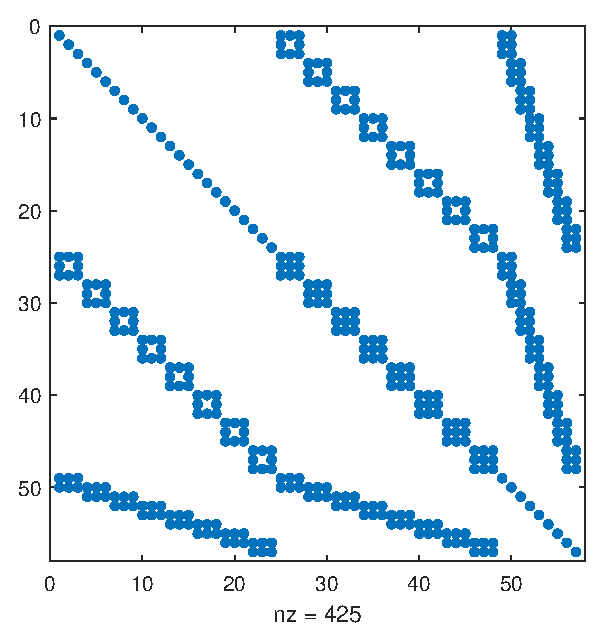
\includegraphics[width=\linewidth]{includefiles/1D poisson HDG spy/legendre direct.eps}
				\caption{original matrix}
			\end{center}
		\end{subfigure}
		\begin{subfigure}{0.49\linewidth}
			\begin{center}
				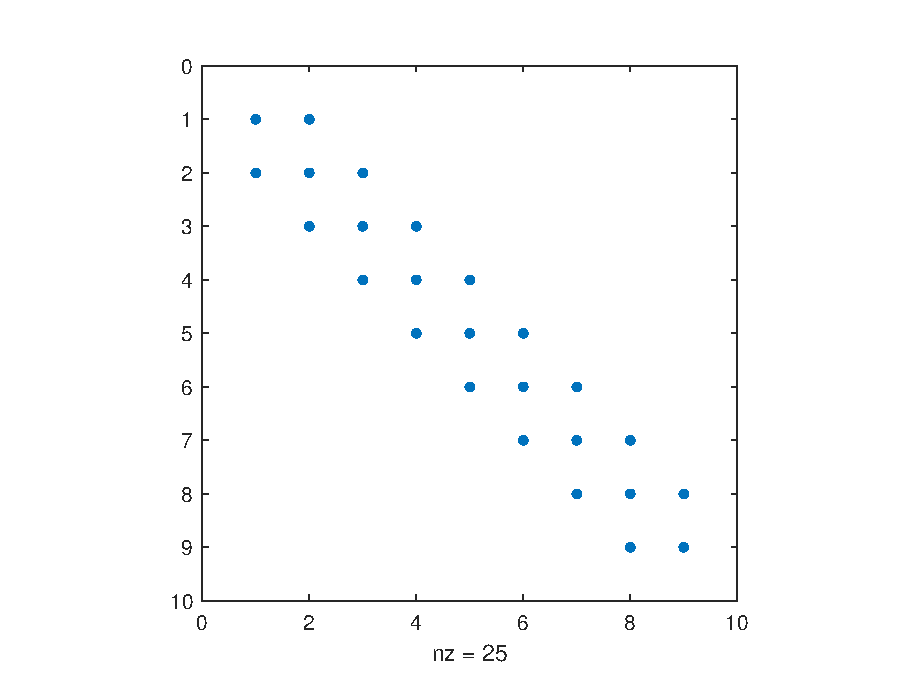
\includegraphics[width=\linewidth]{includefiles/1D poisson HDG spy/legendre reduce.eps}
				\caption{condensed matrix \(\mathbb{K}\)}
			\end{center}
		\end{subfigure}
		\caption{Legendre nodes, \(k = 2\), \(N = 8\)}
		\label{1D LDG-H Legendre node spy}
	\end{center}
\end{figure}

\begin{figure}[H]
	\begin{center}
		\begin{subfigure}{0.49\linewidth}
			\begin{center}
				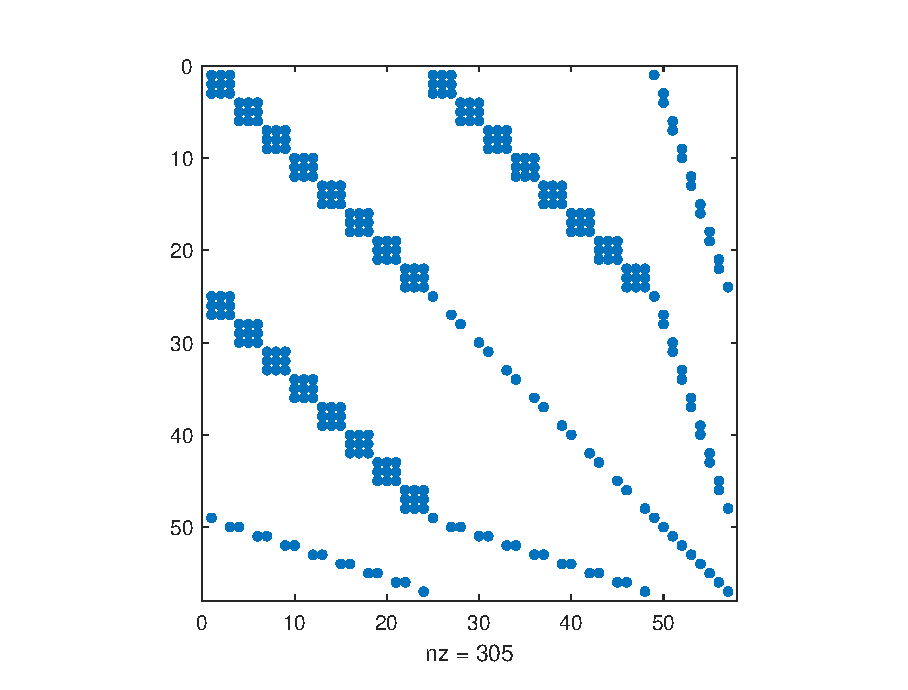
\includegraphics[width=\linewidth]{includefiles/1D poisson HDG spy/lobatto direct.eps}
				\caption{original matrix}
			\end{center}
		\end{subfigure}
		\begin{subfigure}{0.49\linewidth}
			\begin{center}
				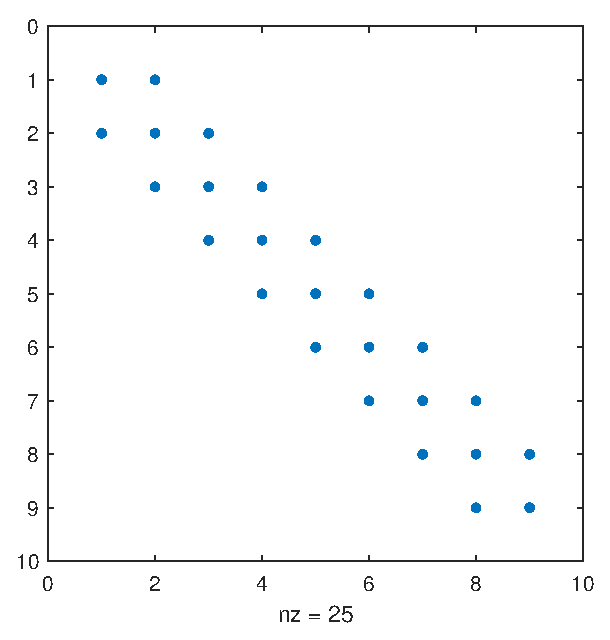
\includegraphics[width=\linewidth]{includefiles/1D poisson HDG spy/lobatto reduce.eps}
				\caption{condensed matrix \(\mathbb{K}\)}
			\end{center}
		\end{subfigure}
		\caption{Lobatto nodes, \(k = 2\), \(N = 8\)}
		\label{1D LDG-H Lobatto node spy}
	\end{center}
\end{figure}


\subsubsection{Numerical Example 2 (Neumann)}

区域 \(\Omega = [0,3\pi]\)，准确解 \(u(x) = \exp\left(\sin(x)\right)\)，采用纯 Neumann 边界条件。空间剖分使用均匀网格，用 \(N\) 表示单元个数，\(k\) 表示多项式次数。取罚参数 \(\tau = 10\). 我们使用 Lobatto 配点法，并使用相同点数的 Gauss-Legendre 公式进行源项 \(f\) 的数值积分和误差测量。通过添加 Lagrange 乘子\cite{10.1007/BF01436561}，该问题的方程组为：
\begin{equation}
	\begin{aligned}
		& \text{find \(\left(\sigma_{h}, u_{h}, \widehat{u}_{h}\right) \in \Sigma_{h}\times V_{h}\times M_{h}\) such that \(\forall \left(\tau_{h}, v_{h}, \widetilde{\mu}_{h}, \mu_{h}^{D}\right)\in\Sigma_{h}\times V_{h} \times \widetilde{M}_{h} \times M_{h}^{D}\):} \\
		& \begin{cases}
			\sum_{K \in \mathcal{T}_{h}} \int_{K} \sigma_h \cdot \tau_{h} \d x + \sum_{K \in \mathcal{T}_{h}} \int_{K} u_{h} \nabla\cdot\tau_{h} \d x - \sum_{K \in \mathcal{T}_{h}} \oint_{\partial K} \widehat{u}_{h} \tau_{h} \cdot \bm n \d s = 0 \\
			\sum_{K \in \mathcal{T}_{h}} \int_{K} \sigma_{h} \cdot \nabla v_{h} \d x - \sum_{K \in \mathcal{T}_{h}} \oint_{\partial K} v_{h} \widehat{\sigma}_{h} \cdot \bm n \d s + \sum_{K \in \mathcal{T}_{h}} \int_{K} \lambda v_{h} \d x = \sum_{K \in \mathcal{T}_{h}} \int_{K} f v_{h} \d x \\
			\sum_{K \in \mathcal{T}_{h}} \oint_{\partial K} \widetilde{\mu}_{h} \widehat{\sigma}_{h} \cdot \bm n \d s = \int_{\Gamma^{N}} \mu_{h} \bm g_{N} \cdot \bm n \d s \\
			\sum_{K \in \mathcal{T}_{h}} \oint_{\partial K} \mu_{h}^{D} \widehat{u}_{h} \d s = \int_{\Gamma^{D}} \mu_{h}^{D} g_{D} \d s \\
			\sum_{K \in \mathcal{T}_{h}} \int_{K} \xi u_{h} = c_0
		\end{cases}
	\end{aligned}
\end{equation}
这里，\(c_0 \in \R\) 可以任取。为了方便测试收敛阶，我们取
\begin{equation}
	c_0 = \int_{\Omega} u(x) \d x \approx 14.16368455672395547087675939170498
\end{equation}
测试结果如表所示：

\begin{table}[H]
	\begin{center}
		\begin{tabular}{c | c c | c c | c c }
			\toprule

			\(N\) & \(\norm{u - u_{h}}_{L^2}\) & order & \(\norm{\sigma -\sigma_{h}}_{L^2}\) & order & \(\norm{u|_{\Gamma} - \widehat{u}_{h}}_{L^2(\Gamma, h)}\) & order \\

			\midrule

			16 & 1.8449e+00 & - & 2.3290e+00 & - & 1.9155e+00 & - \\
			32 & 1.4743e+00 & 0.3236 & 1.8365e+00 & 0.3427 & 1.5086e+00 & 0.3445 \\
			64 & 1.0508e+00 & 0.4885 & 1.2997e+00 & 0.4987 & 1.0683e+00 & 0.4978 \\
			128 & 6.6714e-01 & 0.6554 & 8.2220e-01 & 0.6607 & 6.7623e-01 & 0.6598 \\
			256 & 3.8553e-01 & 0.7911 & 4.7427e-01 & 0.7938 & 3.9022e-01 & 0.7932 \\
			512 & 2.0904e-01 & 0.8831 & 2.5692e-01 & 0.8844 & 2.1143e-01 & 0.8841 \\
			1024 & 1.0913e-01 & 0.9378 & 1.3406e-01 & 0.9384 & 1.1033e-01 & 0.9383 \\
			2048 & 5.5793e-02 & 0.9679 & 6.8525e-02 & 0.9682 & 5.6400e-02 & 0.9681 \\
			4096 & 2.8214e-02 & 0.9837 & 3.4649e-02 & 0.9838 & 2.8519e-02 & 0.9838 \\

			\bottomrule
		\end{tabular}
		\caption{\(k = 0\), \(\tau = 10.0\)}
	\end{center}
\end{table}

\begin{table}[H]
	\begin{center}
		\begin{tabular}{c | c c | c c | c c }
			\toprule

			\(N\) & \(\norm{u - u_{h}}_{L^2}\) & order & \(\norm{\sigma -\sigma_{h}}_{L^2}\) & order & \(\norm{u|_{\Gamma} - \widehat{u}_{h}}_{L^2(\Gamma, h)}\) & order \\

			\midrule

			16 & 7.2958e-02 & - & 3.3565e-01 & - & 9.7459e-03 & - \\
			32 & 1.5574e-02 & 2.2280 & 1.1112e-01 & 1.5949 & 1.5773e-03 & 2.6273 \\
			64 & 3.4712e-03 & 2.1656 & 3.3075e-02 & 1.7483 & 2.3389e-04 & 2.7535 \\
			128 & 8.2328e-04 & 2.0760 & 9.1395e-03 & 1.8555 & 3.2299e-05 & 2.8563 \\
			256 & 2.0225e-04 & 2.0253 & 2.4121e-03 & 1.9218 & 4.2623e-06 & 2.9218 \\
			512 & 5.0324e-05 & 2.0068 & 6.2031e-04 & 1.9592 & 5.4811e-07 & 2.9591 \\

			\bottomrule
		\end{tabular}
		\caption{\(k = 1\), \(\tau = 10.0\)}
	\end{center}
\end{table}

\begin{table}[H]
	\begin{center}
		\begin{tabular}{c | c c | c c | c c }
			\toprule

			\(N\) & \(\norm{u - u_{h}}_{L^2}\) & order & \(\norm{\sigma -\sigma_{h}}_{L^2}\) & order & \(\norm{u|_{\Gamma} - \widehat{u}_{h}}_{L^2(\Gamma, h)}\) & order \\

			\midrule

			8 & 3.5692e-02 & - & 1.6989e-01 & - & 2.9221e-03 & - \\
			16 & 5.0279e-03 & 2.8276 & 3.3787e-02 & 2.3300 & 1.3657e-05 & 7.7413 \\
			32 & 5.9132e-04 & 3.0879 & 5.1822e-03 & 2.7048 & 1.8701e-07 & 6.1903 \\
			64 & 7.1815e-05 & 3.0416 & 7.2736e-04 & 2.8328 & 2.8168e-09 & 6.0530 \\
			128 & 8.8954e-06 & 3.0131 & 9.6807e-05 & 2.9095 & 4.3598e-11 & 6.0137 \\
			256 & 1.1097e-06 & 3.0029 & 1.2504e-05 & 2.9527 & 6.7992e-13 & 6.0027 \\

			\bottomrule
		\end{tabular}
		\caption{\(k = 2\), \(\tau = 10.0\)}
	\end{center}
\end{table}

\begin{table}[H]
	\begin{center}
		\begin{tabular}{c | c c | c c | c c }
			\toprule

			\(N\) & \(\norm{u - u_{h}}_{L^2}\) & order & \(\norm{\sigma -\sigma_{h}}_{L^2}\) & order & \(\norm{u|_{\Gamma} - \widehat{u}_{h}}_{L^2(\Gamma, h)}\) & order \\

			\midrule

			4 & 8.0034e-02 & - & 3.1109e-01 & - & 2.6674e-02 & - \\
			8 & 7.4222e-03 & 3.4307 & 3.9878e-02 & 2.9637 & 1.1008e-04 & 7.9207 \\
			16 & 3.7893e-04 & 4.2918 & 2.9232e-03 & 3.7700 & 8.8063e-08 & 10.2878 \\
			32 & 2.3111e-05 & 4.0353 & 2.1418e-04 & 3.7706 & 3.0961e-10 & 8.1519 \\
			64 & 1.4317e-06 & 4.0128 & 1.4584e-05 & 3.8764 & 1.1543e-12 & 8.0673 \\
			128 & 8.9325e-08 & 4.0025 & 9.5333e-07 & 3.9352 & 1.5829e-13 & 2.8665 \\

			\bottomrule
		\end{tabular}
		\caption{\(k = 3\), \(\tau = 10.0\)}
	\end{center}
\end{table}

\begin{table}[H]
	\begin{center}
		\begin{tabular}{c | c c | c c | c c }
			\toprule

			\(N\) & \(\norm{u - u_{h}}_{L^2}\) & order & \(\norm{\sigma -\sigma_{h}}_{L^2}\) & order & \(\norm{u|_{\Gamma} - \widehat{u}_{h}}_{L^2(\Gamma, h)}\) & order \\

			\midrule

			4 & 3.0730e-02 & - & 1.1477e-01 & - & 2.4473e-03 & - \\
			8 & 6.3434e-04 & 5.5982 & 4.5334e-03 & 4.6620 & 2.9442e-06 & 9.6991 \\
			16 & 2.7578e-05 & 4.5237 & 2.2936e-04 & 4.3049 & 4.4268e-10 & 12.6993 \\
			32 & 8.6226e-07 & 4.9992 & 8.2040e-06 & 4.8051 & 4.1872e-13 & 10.0461 \\
			64 & 2.6948e-08 & 4.9999 & 2.7441e-07 & 4.9019 & 9.8380e-14 & 2.0895 \\
			128 & 8.4312e-10 & 4.9983 & 8.8774e-09 & 4.9501 & 2.2925e-14 & 2.1014 \\

			\bottomrule
		\end{tabular}
		\caption{\(k = 4\), \(\tau = 10.0\)}
	\end{center}
\end{table}

数值结果符合估计，达到了 \((k+1, k+1)\) 阶收敛，同时，\(\widehat{u}_{h}\) 在 \(k\geqslant 1\) 时出现了超收敛。我们下面对源项 \(f\) 的积分使用不同阶的 Gauss-Lobatto 数值积分以测试 \(\widehat{u}_{h}\) 对 \(u\big|_{\Gamma}\) 的超收敛现象。

\begin{table}[H]
	\begin{center}
		\begin{tabular}{c | c c | c c | c c }
			\toprule

			\(N\) & \(\norm{u - u_{h}}_{L^2}\) & order & \(\norm{\sigma -\sigma_{h}}_{L^2}\) & order & \(\norm{u|_{\Gamma} - \widehat{u}_{h}}_{L^2(\Gamma, h)}\) & order \\

			\midrule

			2 & 2.3065e+00 & - & 3.7891e+00 & - & 2.9465e+00 & - \\
			4 & 1.4801e+00 & 0.6401 & 2.1408e+00 & 0.8237 & 4.4621e-01 & 2.7232 \\
			8 & 3.5533e-01 & 2.0584 & 9.0773e-01 & 1.2378 & 5.2887e-02 & 3.0767 \\
			16 & 7.3649e-02 & 2.2704 & 3.3549e-01 & 1.4360 & 9.6112e-03 & 2.4601 \\
			32 & 1.5611e-02 & 2.2381 & 1.1111e-01 & 1.5943 & 1.5745e-03 & 2.6098 \\
			64 & 3.4727e-03 & 2.1684 & 3.3074e-02 & 1.7482 & 2.3382e-04 & 2.7514 \\
			128 & 8.2333e-04 & 2.0765 & 9.1395e-03 & 1.8555 & 3.2297e-05 & 2.8559 \\
			256 & 2.0225e-04 & 2.0253 & 2.4121e-03 & 1.9218 & 4.2623e-06 & 2.9217 \\
			512 & 5.0324e-05 & 2.0068 & 6.2031e-04 & 1.9592 & 5.4811e-07 & 2.9591 \\

			\bottomrule
		\end{tabular}
		\caption{\(k = 1\), \(\tau = 10.0\), 5-point Gauss-Lobatto quadrature}
	\end{center}
\end{table}







\begin{table}[H]
	\begin{center}
		\begin{tabular}{c | c c | c c | c c }
			\toprule

			\(N\) & \(\norm{u - u_{h}}_{L^2}\) & order & \(\norm{\sigma -\sigma_{h}}_{L^2}\) & order & \(\norm{u|_{\Gamma} - \widehat{u}_{h}}_{L^2(\Gamma, h)}\) & order \\

			\midrule

			2 & 7.3475e+00 & - & 4.9321e+00 & - & 1.3597e+01 & - \\
			4 & 5.5459e+00 & 0.4058 & 3.9746e+00 & 0.3114 & 6.7851e+00 & 1.0029 \\
			8 & 4.5209e-01 & 3.6167 & 1.4265e+00 & 1.4784 & 5.2729e-01 & 3.6857 \\
			16 & 1.0224e-01 & 2.1446 & 6.7685e-01 & 1.0755 & 1.2140e-01 & 2.1188 \\
			32 & 3.7582e-02 & 1.4439 & 3.3274e-01 & 1.0245 & 2.8754e-02 & 2.0780 \\
			64 & 1.5822e-02 & 1.2481 & 1.6542e-01 & 1.0082 & 7.0748e-03 & 2.0230 \\
			128 & 7.1614e-03 & 1.1436 & 8.2559e-02 & 1.0027 & 1.7595e-03 & 2.0075 \\
			256 & 3.3895e-03 & 1.0792 & 4.1257e-02 & 1.0008 & 4.3903e-04 & 2.0028 \\
			512 & 1.6464e-03 & 1.0418 & 2.0626e-02 & 1.0002 & 1.0967e-04 & 2.0011 \\

			\bottomrule
		\end{tabular}
		\caption{\(k = 2\), \(\tau = 10.0\), 2-point Gauss-Lobatto quadrature}
	\end{center}
\end{table}

\begin{table}[H]
	\begin{center}
		\begin{tabular}{c | c c | c c | c c }
			\toprule

			\(N\) & \(\norm{u - u_{h}}_{L^2}\) & order & \(\norm{\sigma -\sigma_{h}}_{L^2}\) & order & \(\norm{u|_{\Gamma} - \widehat{u}_{h}}_{L^2(\Gamma, h)}\) & order \\

			\midrule

			2 & 5.1864e+00 & - & 3.1811e+00 & - & 8.1864e+00 & - \\
			4 & 2.0327e+00 & 1.3513 & 1.5928e+00 & 0.9980 & 2.2392e+00 & 1.8703 \\
			8 & 1.0952e-01 & 4.2142 & 2.7306e-01 & 2.5443 & 6.7388e-02 & 5.0543 \\
			16 & 7.0602e-03 & 3.9553 & 4.1432e-02 & 2.7204 & 2.1761e-03 & 4.9527 \\
			32 & 7.3631e-04 & 3.2613 & 5.9521e-03 & 2.7993 & 1.2431e-04 & 4.1297 \\
			64 & 8.5652e-05 & 3.1038 & 8.1004e-04 & 2.8773 & 7.6047e-06 & 4.0309 \\
			128 & 1.0410e-05 & 3.0405 & 1.0620e-04 & 2.9312 & 4.7275e-07 & 4.0078 \\
			256 & 1.2868e-06 & 3.0162 & 1.3617e-05 & 2.9634 & 2.9506e-08 & 4.0020 \\
			512 & 1.6008e-07 & 3.0069 & 1.7245e-06 & 2.9811 & 1.8434e-09 & 4.0006 \\

			\bottomrule
		\end{tabular}
		\caption{\(k = 2\), \(\tau = 10.0\), 3-point Gauss-Lobatto quadrature}
	\end{center}
\end{table}

\begin{table}[H]
	\begin{center}
		\begin{tabular}{c | c c | c c | c c }
			\toprule

			\(N\) & \(\norm{u - u_{h}}_{L^2}\) & order & \(\norm{\sigma -\sigma_{h}}_{L^2}\) & order & \(\norm{u|_{\Gamma} - \widehat{u}_{h}}_{L^2(\Gamma, h)}\) & order \\

			\midrule

			2 & 2.2935e+00 & - & 2.5490e+00 & - & 5.9608e+00 & - \\
			4 & 2.9555e-01 & 2.9561 & 7.3917e-01 & 1.7860 & 2.9682e-01 & 4.3278 \\
			8 & 3.5684e-02 & 3.0500 & 1.6988e-01 & 2.1214 & 3.8116e-03 & 6.2831 \\
			16 & 5.0156e-03 & 2.8308 & 3.3772e-02 & 2.3306 & 1.8144e-05 & 7.7147 \\
			32 & 5.9102e-04 & 3.0851 & 5.1819e-03 & 2.7043 & 2.4912e-07 & 6.1865 \\
			64 & 7.1806e-05 & 3.0410 & 7.2735e-04 & 2.8328 & 3.7549e-09 & 6.0520 \\
			128 & 8.8952e-06 & 3.0130 & 9.6807e-05 & 2.9095 & 5.8123e-11 & 6.0135 \\
			256 & 1.1097e-06 & 3.0029 & 1.2504e-05 & 2.9527 & 9.1227e-13 & 5.9935 \\

			\bottomrule
		\end{tabular}
		\caption{\(k = 2\), \(\tau = 10.0\), 4-point Gauss-Lobatto quadrature}
	\end{center}
\end{table}

\begin{table}[H]
	\begin{center}
		\begin{tabular}{c | c c | c c | c c }
			\toprule

			\(N\) & \(\norm{u - u_{h}}_{L^2}\) & order & \(\norm{\sigma -\sigma_{h}}_{L^2}\) & order & \(\norm{u|_{\Gamma} - \widehat{u}_{h}}_{L^2(\Gamma, h)}\) & order \\

			\midrule

			2 & 2.6439e+00 & - & 1.6736e+00 & - & 1.9258e+00 & - \\
			4 & 3.0357e-01 & 3.1226 & 7.3614e-01 & 1.1849 & 3.2073e-02 & 5.9080 \\
			8 & 3.5369e-02 & 3.1015 & 1.6967e-01 & 2.1172 & 1.3598e-04 & 7.8819 \\
			16 & 5.0224e-03 & 2.8160 & 3.3780e-02 & 2.3285 & 1.0985e-07 & 10.2735 \\
			32 & 5.9119e-04 & 3.0867 & 5.1820e-03 & 2.7046 & 3.8679e-10 & 8.1498 \\
			64 & 7.1811e-05 & 3.0413 & 7.2735e-04 & 2.8328 & 1.4404e-12 & 8.0689 \\

			\bottomrule
		\end{tabular}
		\caption{\(k = 2\), \(\tau = 10.0\), 5-point Gauss-Lobatto quadrature}
	\end{center}
\end{table}






\begin{table}[H]
	\begin{center}
		\begin{tabular}{c | c c | c c | c c }
			\toprule

			\(N\) & \(\norm{u - u_{h}}_{L^2}\) & order & \(\norm{\sigma -\sigma_{h}}_{L^2}\) & order & \(\norm{u|_{\Gamma} - \widehat{u}_{h}}_{L^2(\Gamma, h)}\) & order \\

			\midrule

			2 & 7.0772e+00 & - & 5.2853e+00 & - & 1.3597e+01 & - \\
			4 & 5.5337e+00 & 0.3549 & 4.0092e+00 & 0.3987 & 6.7851e+00 & 1.0029 \\
			8 & 4.2169e-01 & 3.7140 & 1.4812e+00 & 1.4366 & 5.2729e-01 & 3.6857 \\
			16 & 7.3317e-02 & 2.5239 & 7.3140e-01 & 1.0180 & 1.2140e-01 & 2.1188 \\
			32 & 1.8169e-02 & 2.0127 & 3.7482e-01 & 0.9644 & 2.8754e-02 & 2.0780 \\
			64 & 4.5994e-03 & 1.9820 & 1.9166e-01 & 0.9677 & 7.0748e-03 & 2.0230 \\
			128 & 1.1607e-03 & 1.9864 & 9.7134e-02 & 0.9805 & 1.7595e-03 & 2.0075 \\
			256 & 2.9175e-04 & 1.9922 & 4.8924e-02 & 0.9894 & 4.3903e-04 & 2.0028 \\
			512 & 7.3148e-05 & 1.9958 & 2.4555e-02 & 0.9945 & 1.0967e-04 & 2.0011 \\

			\bottomrule
		\end{tabular}
		\caption{\(k = 3\), \(\tau = 10.0\), 2-point Gauss-Lobatto quadrature}
	\end{center}
\end{table}

\begin{table}[H]
	\begin{center}
		\begin{tabular}{c | c c | c c | c c }
			\toprule

			\(N\) & \(\norm{u - u_{h}}_{L^2}\) & order & \(\norm{\sigma -\sigma_{h}}_{L^2}\) & order & \(\norm{u|_{\Gamma} - \widehat{u}_{h}}_{L^2(\Gamma, h)}\) & order \\

			\midrule

			2 & 4.9611e+00 & - & 3.7880e+00 & - & 8.1864e+00 & - \\
			4 & 2.0362e+00 & 1.2848 & 1.6104e+00 & 1.2340 & 2.2392e+00 & 1.8703 \\
			8 & 1.1782e-01 & 4.1112 & 3.3862e-01 & 2.2497 & 6.7388e-02 & 5.0543 \\
			16 & 1.3752e-02 & 3.0990 & 8.8972e-02 & 1.9282 & 2.1761e-03 & 4.9527 \\
			32 & 2.5421e-03 & 2.4355 & 2.2168e-02 & 2.0049 & 1.2431e-04 & 4.1297 \\
			64 & 5.4469e-04 & 2.2225 & 5.5345e-03 & 2.0019 & 7.6047e-06 & 4.0309 \\
			128 & 1.2603e-04 & 2.1117 & 1.3830e-03 & 2.0007 & 4.7275e-07 & 4.0078 \\
			256 & 3.0327e-05 & 2.0551 & 3.4569e-04 & 2.0002 & 2.9506e-08 & 4.0020 \\
			512 & 7.4406e-06 & 2.0271 & 8.6420e-05 & 2.0001 & 1.8434e-09 & 4.0005 \\

			\bottomrule
		\end{tabular}
		\caption{\(k = 3\), \(\tau = 10.0\), 3-point Gauss-Lobatto quadrature}
	\end{center}
\end{table}

\begin{table}[H]
	\begin{center}
		\begin{tabular}{c | c c | c c | c c }
			\toprule

			\(N\) & \(\norm{u - u_{h}}_{L^2}\) & order & \(\norm{\sigma -\sigma_{h}}_{L^2}\) & order & \(\norm{u|_{\Gamma} - \widehat{u}_{h}}_{L^2(\Gamma, h)}\) & order \\

			\midrule

			2 & 4.1047e+00 & - & 3.2614e+00 & - & 5.9608e+00 & - \\
			4 & 2.9464e-01 & 3.8002 & 4.8996e-01 & 2.7347 & 2.9682e-01 & 4.3278 \\
			8 & 1.0769e-02 & 4.7740 & 4.6606e-02 & 3.3941 & 3.8116e-03 & 6.2831 \\
			16 & 4.8538e-04 & 4.4716 & 3.4031e-03 & 3.7756 & 1.8144e-05 & 7.7147 \\
			32 & 2.7948e-05 & 4.1183 & 2.3948e-04 & 3.8289 & 2.4912e-07 & 6.1865 \\
			64 & 1.6915e-06 & 4.0463 & 1.5974e-05 & 3.9061 & 3.7549e-09 & 6.0520 \\
			128 & 1.0440e-07 & 4.0181 & 1.0335e-06 & 3.9501 & 5.8130e-11 & 6.0133 \\
			256 & 6.4915e-09 & 4.0074 & 6.5764e-08 & 3.9741 & 9.2658e-13 & 5.9712 \\

			\bottomrule
		\end{tabular}
		\caption{\(k = 3\), \(\tau = 10.0\), 4-point Gauss-Lobatto quadrature}
	\end{center}
\end{table}

\begin{table}[H]
	\begin{center}
		\begin{tabular}{c | c c | c c | c c }
			\toprule

			\(N\) & \(\norm{u - u_{h}}_{L^2}\) & order & \(\norm{\sigma -\sigma_{h}}_{L^2}\) & order & \(\norm{u|_{\Gamma} - \widehat{u}_{h}}_{L^2(\Gamma, h)}\) & order \\

			\midrule

			2 & 1.7294e+00 & - & 2.1477e+00 & - & 1.9258e+00 & - \\
			4 & 8.3175e-02 & 4.3779 & 3.1208e-01 & 2.7828 & 3.2073e-02 & 5.9080 \\
			8 & 7.3784e-03 & 3.4948 & 3.9756e-02 & 2.9727 & 1.3598e-04 & 7.8819 \\
			16 & 3.7829e-04 & 4.2857 & 2.9221e-03 & 3.7661 & 1.0985e-07 & 10.2735 \\
			32 & 2.3101e-05 & 4.0335 & 2.1417e-04 & 3.7702 & 3.8679e-10 & 8.1498 \\
			64 & 1.4315e-06 & 4.0123 & 1.4583e-05 & 3.8764 & 1.4424e-12 & 8.0670 \\

			\bottomrule
		\end{tabular}
		\caption{\(k = 3\), \(\tau = 10.0\), 5-point Gauss-Lobatto quadrature}
	\end{center}
\end{table}







\begin{table}[H]
	\begin{center}
		\begin{tabular}{c | c c | c c | c c }
			\toprule

			\(N\) & \(\norm{u - u_{h}}_{L^2}\) & order & \(\norm{\sigma -\sigma_{h}}_{L^2}\) & order & \(\norm{u|_{\Gamma} - \widehat{u}_{h}}_{L^2(\Gamma, h)}\) & order \\

			\midrule

			2 & 7.0965e+00 & - & 5.1390e+00 & - & 1.3597e+01 & - \\
			4 & 5.5349e+00 & 0.3586 & 4.0358e+00 & 0.3486 & 6.7851e+00 & 1.0029 \\
			8 & 4.0526e-01 & 3.7716 & 1.4867e+00 & 1.4408 & 5.2729e-01 & 3.6857 \\
			16 & 6.6662e-02 & 2.6039 & 6.9297e-01 & 1.1012 & 1.2140e-01 & 2.1188 \\
			32 & 2.2540e-02 & 1.5644 & 3.3487e-01 & 1.0492 & 2.8754e-02 & 2.0780 \\
			64 & 9.9616e-03 & 1.1780 & 1.6567e-01 & 1.0153 & 7.0748e-03 & 2.0230 \\
			128 & 4.8175e-03 & 1.0481 & 8.2587e-02 & 1.0043 & 1.7595e-03 & 2.0075 \\
			256 & 2.3883e-03 & 1.0123 & 4.1261e-02 & 1.0011 & 4.3903e-04 & 2.0028 \\
			512 & 1.1916e-03 & 1.0031 & 2.0626e-02 & 1.0003 & 1.0967e-04 & 2.0011 \\

			\bottomrule
		\end{tabular}
		\caption{\(k = 4\), \(\tau = 10.0\), 2-point Gauss-Lobatto quadrature}
	\end{center}
\end{table}

\begin{table}[H]
	\begin{center}
		\begin{tabular}{c | c c | c c | c c }
			\toprule

			\(N\) & \(\norm{u - u_{h}}_{L^2}\) & order & \(\norm{\sigma -\sigma_{h}}_{L^2}\) & order & \(\norm{u|_{\Gamma} - \widehat{u}_{h}}_{L^2(\Gamma, h)}\) & order \\

			\midrule

			2 & 5.0187e+00 & - & 3.5348e+00 & - & 8.1864e+00 & - \\
			4 & 2.0697e+00 & 1.2779 & 1.8255e+00 & 0.9533 & 2.2392e+00 & 1.8703 \\
			8 & 1.4848e-01 & 3.8010 & 5.9325e-01 & 1.6216 & 6.7388e-02 & 5.0543 \\
			16 & 3.4016e-02 & 2.1260 & 2.6436e-01 & 1.1661 & 2.1761e-03 & 4.9527 \\
			32 & 1.3655e-02 & 1.3168 & 1.2777e-01 & 1.0490 & 1.2431e-04 & 4.1297 \\
			64 & 6.1660e-03 & 1.1470 & 6.3245e-02 & 1.0145 & 7.6047e-06 & 4.0309 \\
			128 & 2.9278e-03 & 1.0745 & 3.1535e-02 & 1.0040 & 4.7275e-07 & 4.0078 \\
			256 & 1.4262e-03 & 1.0377 & 1.5756e-02 & 1.0010 & 2.9506e-08 & 4.0020 \\
			512 & 7.0380e-04 & 1.0189 & 7.8767e-03 & 1.0003 & 1.8434e-09 & 4.0005 \\

			\bottomrule
		\end{tabular}
		\caption{\(k = 4\), \(\tau = 10.0\), 3-point Gauss-Lobatto quadrature}
	\end{center}
\end{table}

\begin{table}[H]
	\begin{center}
		\begin{tabular}{c | c c | c c | c c }
			\toprule

			\(N\) & \(\norm{u - u_{h}}_{L^2}\) & order & \(\norm{\sigma -\sigma_{h}}_{L^2}\) & order & \(\norm{u|_{\Gamma} - \widehat{u}_{h}}_{L^2(\Gamma, h)}\) & order \\

			\midrule

			2 & 4.1029e+00 & - & 3.0120e+00 & - & 5.9608e+00 & - \\
			4 & 3.0188e-01 & 3.7646 & 5.1659e-01 & 2.5436 & 2.9682e-01 & 4.3278 \\
			8 & 1.6953e-02 & 4.1544 & 8.3557e-02 & 2.6282 & 3.8116e-03 & 6.2831 \\
			16 & 1.2453e-03 & 3.7670 & 9.3841e-03 & 3.1545 & 1.8144e-05 & 7.7147 \\
			32 & 1.2867e-04 & 3.2747 & 1.1833e-03 & 2.9874 & 2.4912e-07 & 6.1865 \\
			64 & 1.4526e-05 & 3.1469 & 1.4821e-04 & 2.9971 & 3.7549e-09 & 6.0520 \\
			128 & 1.7232e-06 & 3.0755 & 1.8534e-05 & 2.9994 & 5.8126e-11 & 6.0134 \\
			256 & 2.0980e-07 & 3.0380 & 2.3170e-06 & 2.9999 & 9.1031e-13 & 5.9967 \\

			\bottomrule
		\end{tabular}
		\caption{\(k = 4\), \(\tau = 10.0\), 4-point Gauss-Lobatto quadrature}
	\end{center}
\end{table}

\begin{table}[H]
	\begin{center}
		\begin{tabular}{c | c c | c c | c c }
			\toprule

			\(N\) & \(\norm{u - u_{h}}_{L^2}\) & order & \(\norm{\sigma -\sigma_{h}}_{L^2}\) & order & \(\norm{u|_{\Gamma} - \widehat{u}_{h}}_{L^2(\Gamma, h)}\) & order \\

			\midrule

			2 & 1.8092e+00 & - & 1.6380e+00 & - & 1.9258e+00 & - \\
			4 & 5.1678e-02 & 5.1296 & 1.4657e-01 & 3.4822 & 3.2073e-02 & 5.9080 \\
			8 & 1.1194e-03 & 5.5288 & 6.2650e-03 & 4.5482 & 1.3598e-04 & 7.8819 \\
			16 & 3.4741e-05 & 5.0099 & 2.6477e-04 & 4.5645 & 1.0985e-07 & 10.2735 \\
			32 & 1.0477e-06 & 5.0513 & 9.1492e-06 & 4.8550 & 3.8679e-10 & 8.1498 \\
			64 & 3.2249e-08 & 5.0219 & 3.0090e-07 & 4.9263 & 1.4410e-12 & 8.0683 \\

			\bottomrule
		\end{tabular}
		\caption{\(k = 4\), \(\tau = 10.0\), 5-point Gauss-Lobatto quadrature}
	\end{center}
\end{table}


\subsubsection{Conclusion}

我们编程实现了一维 Poisson 方程的 Dirichlet 两点边值问题以及纯 Neumann 边值问题的 LDG-H 方法，该方法通过以边界数值通量 \(\widehat{u}_{h}\) 作为变量进行杂交化，可以在很大程度上减少全局相互耦合的方程组自由度个数。我们的测试显示出对 \((\sigma, u)\) 的 \((k+1, k+1)\) 阶收敛，达到了最优，且与理论结果一致。同时，在 Dirichlet 两点边值问题中，当 \(k \geqslant 1\) 时，我们验证了 \(u\big|_{\Gamma}\) 的求解是精确的这一结论；在纯 Neumann 边值问题中，通过数值实验我们合理地猜测，当 \(k \geqslant 2\) 时，\(u\big|_{\Gamma}\) 的求解是精确的。
